\documentclass[a4paper, twoside, parskip, 10pt, smallheadings]{scrbook}
\input{praeambel_neu}
% Dies ist die Datei makros.tex in der Fassung vom 4. Juli 1997,
% die alle in der Aufgabensammlung enthaltenen Makros und Umgebungen
% enthaelt.
%
% Die Namen aller nur fuer die Aufgabensammlung verwendeten Makros
% werden gross geschrieben.
%
% In den TeX-Blaettern werden die Aufgaben mit dem Makro ABINPUT
% eingelesen, dem der Dateiname mit und ohne geschweifte Klammern
% folgen kann. Der Titel eines Blattes wird mit der Umgebung
% ABTITEL gekennzeichnet, damit es vom Programm zur Auswahl der
% Aufgaben gefunden wird.
%
% Die Quelltexte der Aufgaben duerfen keine INPUT-Anweisungen,
% etwa zum Einlesen von Graphiken, enthalten, da die zugehoerigen
% Dateien vom Programm ABSELECT, das die Auswahl der Aufgaben
% erledigt, nicht gefunden werden.
%
%*********************************************************************************************
%
% Um bei der Verwendung von KOMA-Script (srcbook) bei enumerate (2. Ebene)
% die Doppelklammer im Label zu haben [(a) statt a)] (RR, 2001)
%
\renewcommand*\labelenumii{(\theenumii)}
%
%*********************************************************************************************
%
%% Kopf- und Fusszeilen auf den Blaettern
% Die Makros KOPFTEXT und FUSSTEXT legen Kopf- und Fusszeile jedes
% TeX-Blattes fest. Durch die Leerdefinitionen von KopfU, KopfG usw.
% zu Beginn des Uebersetzungsvorganges ist eine einheitliche Definition
% von Kopf- und Fusszeilen im gesamten zum Ausdruck benoetigten
% TeX-Dokument moeglich.
%---------------------------------------------------------------------------------------------
\newcommand{\KopfU}{}
\newcommand{\KopfG}{}
\newcommand{\FussU}{}
\newcommand{\FussG}{}
\newcommand{\KOPFTEXT}[1]{%
\renewcommand{\KopfU}{\parbox{\textwidth}%
{\sf\small #1 \hfill\thepage\\%
\rule[2ex]{\textwidth}{0.2mm}}}
\renewcommand{\KopfG}{\parbox{\textwidth}%
{\sf\small\thepage\hfill #1\\%
\rule[2ex]{\textwidth}{0.2mm}}}}
% Fusszeile
\newcommand{\FUSSTEXT}[1]{%
\renewcommand{\FussU}{\parbox{\textwidth}%
{\sf\small\rule[-0.9ex]{\textwidth}{0.2mm}\\%
#1 \\%
\rule[2ex]{\textwidth}{0.2mm}}}
\renewcommand{\FussG}{\parbox{\textwidth}%
{\sf\small\rule[-0.9ex]{\textwidth}{0.2mm}\\%
\hfill #1 \\%
\rule[2ex]{\textwidth}{0.2mm}}}
}
%*********************************************************************************************
%
%% ABTITEL
% Diese Umgebung kennzeichnet den Titel eines TeX-Blattes und muss auf
% jedem Blatt vorhanden sein, da das Programm zur Aufgabenauswahl nach
% ABTITEL sucht.
% Der Schalter PRIVATE erlaubt es, beim Gesamtausdruck fuer die
% TeX-Blaetter numerierte Ueberschriften zu erzeugen.
%---------------------------------------------------------------------------------------------
\newif\ifPRIVATE
\PRIVATEfalse
\newenvironment{ABTITEL}{\ifPRIVATE\begin{center}%
\setbox0=\vbox\bgroup\else\begin{center}\bf \large\fi}%
{\ifPRIVATE\egroup\fi\end{center}}%
%*********************************************************************************************
%
%% ABINPUT, FILE
% Das Makro ABINPUT ersetzt die TeX-eigene INPUT-Anweisung und dient
% zum Einlesen des Quelltextes einer Aufgabe. Das Makro uebernimmt ausserdem
% die Funktion des item-Befehls, zeigt also auch die Aufgabennummer auf dem
% jeweiligen Blatt an. Dies hat zur Folge, dass die AUFGABEN-Umgebung ein
% enumerate enthalten muss.
%
% Der Schalter FILE bestimmt, ob die Dateinamen der Aufgaben
% ausgegeben werden. Der Dateiname ist ggf. Teil der Itemmarkierung.
%---------------------------------------------------------------------------------------------
\newif\ifFILE
\def\ABINPUT #1 {%
\ifFILE{\item[\hspace{-2em}{\footnotesize\sf\fbox{#1}}\hspace{2em}%
\addtocounter{enumi}{1}\labelenumi]\input{#1}}%
\else{\item\input{#1}\ }\fi}
%*********************************************************************************************
%
%% AUFGABEN
% Eine Umgebung fuer Aufgaben, zunaechst im Wesentlichen eine Verkleidung
% fuer enumerate, kann aber spaeter weitere Stilmerkmale aufnehmen.
% Gibt zur Zeit den Namen des TeX-Blattes rechts unten auf der letzten
% Seite aus, falls die entsprechenden Anweisungen nicht auskommentiert
% sind.
%---------------------------------------------------------------------------------------------
\newenvironment{AUFGABEN}{\begin{enumerate}}
                         {\end{enumerate}}
                          %\vfill
                          %\hfill\tiny\jobname}
%*********************************************************************************************
%
%% ANG, ANGABE  (RR 2001)
% ANGABE ist eine Boolsche Variable, um zu entscheiden, ob Angaben
% gedruckt werden. ANG ist eine Umgebung fuer Angaben,
% im Wesentlichen, um diese auf Wunsch ein- und ausblenden zu koennen.
%---------------------------------------------------------------------------------------------
\newif\ifANGABE
\newcommand{\ANG}[1]{
    \ifANGABE{#1}\else{}\fi
  }
%*********************************************************************************************
%
%% LSG, LOESUNG
% LOESUNG ist eine Boolsche Variable, um zu entscheiden, ob Loesungen
% gedruckt werden. LSG ist eine Umgebung fuer Loesungen,
% im Wesentlichen, um diese auf Wunsch ein- und ausblenden zu koennen.
% Gelegentlich kann der Loesungstext auch methodische und didaktische
% Hinweise enthalten.
%---------------------------------------------------------------------------------------------
%%\newif\ifLOESUNG
%%\newdimen\mydim
%%\newenvironment{LSG}{\ifLOESUNG{{\it L"osung:}\quad}\else{}\fi%
%%\mydim=\hsize%
%%\advance\mydim by -30mm%
%%\setbox0=\vbox\bgroup\hsize=\mydim\begin{minipage}[t]{0.98\hsize}
%%\begin{small}}%
%%{\end{small}\end{minipage}\egroup\ifLOESUNG{\box0}\else{}\fi}
%
% Diese neue Definition des LSG-Makros erlaubt Seitenumbrueche in der
% Loesung und Loesungen, die laenger als eine Seite sind. 
% Aus typographischen Gruenden wurde der Schriftstil \small
% statt \it gewaehlt. (RR 1998, 2001)
%
\newif\ifLOESUNG
\newcommand{\LSG}[1]%
  { \ifANGABE
      { \ifLOESUNG\begingroup
        \begin{small}
        \begin{list}{\it L�sung:\hfill}%
                { \setlength{\itemindent}{0mm}
                  \setlength{\labelwidth}{14mm}
                  \setlength{\leftmargin}{0mm}
                }
        \item #1
        \end{list}\end{small}\endgroup\else{}\fi
      }
    \else
      { \ifLOESUNG{
        \begin{small}%
        #1
        \end{small}%
        }\else{}\fi%
      }\fi
  }
%%
%
%*********************************************************************************************
%
%% BILD
% Das folgende Makro dient der Einbindung von PCX-Grafiken.
% Diese muessen alle in einem Verzeichnis direkt unterhalb des
% jeweiligen Verzeichnisses fuer die Jahrgangsstufe
% liegen.
% Auch bei den Grafiken muss die Trennung nach Jahrgangsstufen
% beibehalten werden, da jede Jahrgangsstufe gesondert per FTP
% aktualisiert werden koennen muss.
% Da PCX-Bilder recht umfangreich sind und zudem nicht vom WWW-Server
% nicht ohne weiteres uebertragen werden koennen, muss ihre Verwendung
% auf das unbedingt notwendige Mass beschraenkt bleiben.
%---------------------------------------------------------------------------------------------
\newcommand{\BILD}[2]{%
\special{em: graph c:/ab/#1/grf/#2}}
%*********************************************************************************************
% 
%% Einbindung von EPS-Graphiken (RR 1999)
%
\newcommand{\EPSBASIS}[3]{
    \ifthenelse{\equal{#2}{}}
         {\ifthenelse{\equal{#3}{}}
                {}
                {\includegraphics[height=#3]{#1}}
         }
         {\ifthenelse{\equal{#3}{}}
                {\includegraphics[width=#2]{#1}}
                {\includegraphics[width=#2,height=#3]{#1}}
         }
  } 
%
%
%
\newcommand{\EPS}[4]{ \raisebox{2.5mm}{\parbox[t]{#2}{
                          \vspace{0pt}
                          #4
                          \EPSBASIS{#1}{#2}{#3}
                          }}
                        }
%
\newcommand{\EPSB}[4]{ \setlength{\fboxsep}{0pt}
                       \raisebox{2.5mm}{\parbox[t]{#2}{
                          \vspace{0pt}
                          #4
                          \fbox{\EPSBASIS{#1}{#2}{#3}}
                        }}
                       \setlength{\fboxsep}{3pt}
                      }
%
\newcommand{\EPSR}[6]{\parbox[t]{#1}{%\vspace{0pt}
                          #6}\hfill
                          \raisebox{2.5mm}{\parbox[t]{#3}{
                          \vspace{0pt}
                          #5
                          \EPSBASIS{#2}{#3}{#4}
                          }}
                        }
%
\newcommand{\EPSC}[4]{\begin{center}
                            \raisebox{2.5mm}{\parbox[t]{#2}{
                            \vspace{0pt}
                            #4
                            \EPSBASIS{#1}{#2}{#3}
                            }}
                            \end{center}
                           }
%
\newcommand{\EPSRB}[6]{\parbox[t]{#1}{%\vspace{0pt}
                          #6}\hfill
                          \raisebox{2.5mm}{\parbox[t]{#3}{
                          \setlength{\fboxsep}{0pt}
                          \vspace{0pt}
                          #5
                          \fbox{\EPSBASIS{#2}{#3}{#4}}
                          \setlength{\fboxsep}{3pt}
                          }}
                        }
%
\newcommand{\EPSCB}[4]{\begin{center}
                            \raisebox{2.5mm}{\parbox[t]{#2}{
                            \setlength{\fboxsep}{0pt}
                            \vspace{0pt}
                            #4
                            \fbox{\EPSBASIS{#1}{#2}{#3}}
                            \setlength{\fboxsep}{3pt}
                            }}
                            \end{center}
                           }
%
\newcommand{\PSF}[2]{\psfrag{#1}{\scriptsize #2}}
\newcommand{\PSFM}[2]{\psfrag{#1}[][]{\scriptsize #2}}
\newcommand{\PSFROT}[3]{\psfrag{#2}[c][c][1][#1]{\scriptsize #3}}
%
%% AUFZAEHLUNG, TEILAUFGABE, TAG
% Automatisches Durchzaehlen nebeneinander angeordneter Teilaufgaben
% Beispiel \begin{AUFZAEHLUNG}{l}
%          \TEILAUFGABE{......}
%          \end{AUFZAEHLUNG}
%---------------------------------------------------------------------------------------------
\newcounter{TAG}
\newenvironment{AUFZAEHLUNG}[1]{\setcounter{TAG}{1}%
\begin{tabular}{#1}}{\end{tabular}\hspace{-2em}}
%
\newcommand{\ZAEHLE}{\alph{TAG})}
\newcommand{\TEILAUFGABE}[1]{\ZAEHLE\hspace{1em}#1\hspace{1em}%
\addtocounter{TAG}{1}}
%*********************************************************************************************
%
%% PUNKTE
% Das folgende Makro dient dazu, am Rand einer Schulaufgabe die
% Bewertungseinheiten bei jeder Teilaufgabe zu notieren.
%---------------------------------------------------------------------------------------------
\newcommand{\PUNKTE}[1]{\mbox{}\marginpar{\hspace*{1em}\fbox{#1}}}
%*********************************************************************************************
%
%% TIMMS
% Das folgende Makro dient dazu, am Rand der Aufgaben einen Hinweis
% auf die Art der Aufgabe ("neue Aufgabenkultur") zu plazieren.
%---------------------------------------------------------------------------------------------
\newcommand{\TIMMS}[1]{\mbox{}\marginpar{\hspace*{3em}\fbox{#1}}}
%*********************************************************************************************
%
%% EGY
% Aufgaben f"ur das Europ"aische Gymnasium 
% veraltet
%---------------------------------------------------------------------------------------------
%\newcommand{\EGY}{\mbox{}\marginpar[]{\fbox{\small{EGY}}}}
\newcommand{\EGY}{}
%*********************************************************************************************
%
%% D, T, SC, SSC
% Einschalten von Displaystil bzw. Textstil beim Mathematiksatz
%---------------------------------------------------------------------------------------------
\newcommand{\D}{\displaystyle}
\newcommand{\T}{\textstyle}
\newcommand{\SC}{\scriptstyle}
\newcommand{\SSC}{\scriptscriptstyle}
%*********************************************************************************************
%
%% GF
% Anfuehrungszeichen fuer Zitate
%---------------------------------------------------------------------------------------------
\newcommand{\GF}[1]{\glqq{}#1\grqq{}}
%*********************************************************************************************
%
%% VPFEIL
% Zeichen fuer Vektorpfeil, nur im Mathmode verwenden
%---------------------------------------------------------------------------------------------
%\newcommand{\VPFEIL}[1]{\stackrel{\D\longrightarrow}{#1}}
\newcommand{\VPFEIL}[1]{\overrightarrow{#1}}
\newcommand{\VPFEILRM}[1]{\overrightarrow{\mathrm{#1}}}
%*********************************************************************************************
%
%% RVEKTOR, EVEKTOR
% Raeumliche und ebene Spaltenvektoren
\newcommand{\RVEKTOR}[4]{\left(\begin{array}{#1}\negthickspace#2\negthickspace\\\negthickspace#3\negthickspace\\\negthickspace#4\negthickspace\end{array}\right)}
\newcommand{\EVEKTOR}[3]{\left(\begin{array}{#1}\negthickspace#2\negthickspace\\\negthickspace#3\negthickspace\end{array}\right)}
%*********************************************************************************************
%%
%*********************************************************************************************
%
%% EPUNKT, RPUNKT
% Ebene und raeumliche Punktkoordinaten
\newcommand{\EPUNKT}[3]{
  {\rm #1}\left(\,#2\;\vline\;#3\,\right)}
\newcommand{\RPUNKT}[4]{
  {\rm #1}\left(\,#2\;\vline\;#3\;\vline\;#4\,\right)}
%
%*********************************************************************************************
%
%% POLAR
% Polarform komplexer Zahlen in der Form (r|phi)_p
% Verwendung: \POLAR{r}{phi}
\newcommand{\POLAR}[2]{
  \left(\,#1\;\vline\;#2\,\right)_{\mathrm{p}}}
%
%*********************************************************************************************
%
%% POLARE
% Polarform komplexer Zahlen in der Form r E(phi)
% Verwendung: \POLARE{r}{phi}
\newcommand{\POLARE}[2]{
  #1\cdot\mathrm{E}\left(#2\right)}
%
%*********************************************************************************************
%
%% KREIS
% Kreis in der Form k(M;r) im Mathemodus
% Verwendung: \KREIS{M}{r}
\newcommand{\KREIS}[2]{
  \text{k}(\text{#1;}#2)}
\newcommand{\KREISi}[2]{
  \text{k}_{\text{i}}(\text{#1;}#2)}
\newcommand{\KREISa}[2]{
  \text{k}_{\text{a}}(\text{#1;}#2)}
%
%*********************************************************************************************
%
%% DANN (daraus folgt), GENAUDANN
% Das logische Zeichen "daraus folgt" und "genau dann, wenn"
\newcommand{\DANN}{\Longrightarrow}
\newcommand{\GENAUDANN}{\Longleftrightarrow}
%
%*********************************************************************************************
%
%% OHNE (Mengenzeichen)
\newcommand{\OHNE}{\mathrel{\setminus}}
%
%*********************************************************************************************
%
%% SATZB{Zeile1\\Zeile2\\...}
% Ein gerahmter und zentrierter Satz, wobei sich die Rahmenbreite der
% Textbreite anpasst. SATZB{} stellt eine mehrzeilige math-Umgebung
% bereit, die Zeilen sind zentriert. 
% Normaler Text wird mit \text{} eingegeben.
\newcommand{\SATZB}[1]{\begin{displaymath}\boxed{\begin{gathered}
                       #1\end{gathered}}\end{displaymath}}
%
%*********************************************************************************************
%
%% RFRAC{z}{n}
% Bruch in Roman (fuer Einheiten)
\newcommand{\RFRAC}[2]{\frac{\rm #1}{\rm #2}}
%
%*********************************************************************************************
%
%% ggT, kgV
% im mathem. Modus in Roman gesetzt
\newcommand{\ggT}{\mathrm{ggT}}
\newcommand{\kgV}{\mathrm{kgV}}
%
%*********************************************************************************************
%
%% \RMd
% im mathem. Modus in Roman gesetztes d (Differentiale)
\newcommand{\RMd}{\mathrm{d}}
%
%*********************************************************************************************
%
%% EURO und MEUR (EURO im Mathemodus), Ct fuer Cent
\DeclareFontFamily{OT1}{mvs}{}
\DeclareFontShape{OT1}{mvs}{m}{n}{<-> fmvr8x}{}
\def\mvs{\usefont{OT1}{mvs}{m}{n}}
\def\mvchr{\mvs\char}
\def\textmvs#1{{\mvs #1}}
\def\EURhv{{\mvchr99}}\def\EURcr{{\mvchr100}}\def\EURtm{{\mvchr101}}
\def\EUR{{\mvchr164}}
\newcommand{\MEUR}{\mbox{\EUR}}
\newcommand{\Ct}{\ensuremath{\mbox{Ct}}}
%
%*********************************************************************************************
%
%% Mmu
%   aufrechtes mu im Mathemodus
%\newcommand{\Mmu}{\mbox{\textmu}}
\newcommand{\Mmu}{\mu}
%
%*********************************************************************************************
%
%% GC
%  Grad Celsius (im Mathemodus)
\newcommand{\GC}{\,^{\circ}\mathrm{C}}
%
%*********************************************************************************************
%

%
% Neben ein Befehlswort kommt eine \fbox bis Zeilenende
% Beispiel: \FBEFEHL{Beweise:\quad}{Sind ...}
%
\newlength{\LBefehl}
\newlength{\BBefehl}
\newcommand{\FBEFEHL}[2]{\settowidth{\LBefehl}{#1}\setlength{\BBefehl}{\linewidth}%
\addtolength{\BBefehl}{-\LBefehl}%\addtolength{\BBefehl}{-7mm}%
#1\fbox{\parbox[t]{\BBefehl}{#2}}\\}  
% das Gleiche ohne \fbox
\newcommand{\BEFEHL}[2]{\settowidth{\LBefehl}{#1}\setlength{\BBefehl}{\linewidth}%
\addtolength{\BBefehl}{-\LBefehl}%\addtolength{\BBefehl}{-2mm}%
#1\parbox[t]{\BBefehl}{#2}\\} 
%
%*********************************************************************************************
%
\newcommand{\relsqrt}{\sqrt{1-\beta^{2}}}
\newcommand{\relgamma}{\frac{1}{\sqrt{1-\beta^{2}}}}
%
%*********************************************************************************************
%
% Zeichen in einem Kreis
%\newcommand{\IMKREIS}[1]{ \unitlength 1mm 
%                          \begin{picture}(3,3)
%                          \put(1,1){\circle{4}}
%                          \put(1,1){\makebox(0,0){#1}}
%                          \end{picture}
%}
\def\IMKREIS#1{ ${%
	\psset{unit=1pt}
	\setbox0=\hbox{#1}\relax
	\dimen0=\the\wd0\dimen1=\the\ht0
	\divide\dimen0 by 2\divide\dimen1 by 2
	\ifdim\dimen0>\dimen1\dimen2=\dimen0\else\dimen2=\dimen1\fi
	\advance\dimen2 by +5pt
	\rput(\dimen0, \dimen1){\pscircle{\dimen2}}
	\box0%
}$ }
%*********************************************************************************************
%
% plus - nicht minus, nicht plus - minus
\newcommand{\PNM}{\raisebox{-1mm}{$\SC\,\stackrel{+}{(-)}\,$}}
\newcommand{\NPM}{\raisebox{-1mm}{$\SC\,\stackrel{(+)}{-}\,$}}

%
%% \BOX{Breite}{Hoehe}{Zeichen}
%  Zeichen in Box einer festen Breite und Hoehe
\newcommand{\BOX}[3]{\framebox[#1]{\rule[-1.5mm]{0mm}{#2}#3}}
%
%*********************************************************************************************
%% NN, BB, ZZ, QQ, RR, CC, GG, LL, DD, WW
% Makros zur Bezeichnung von Zahlenmengen
%---------------------------------------------------------------------------------------------
\newcommand{\NN}{\mathds{N}}
\newcommand{\BB}{\mathds{B}}
\newcommand{\CC}{\mathds{C}}
\newcommand{\ZZ}{\mathds{Z}}
\newcommand{\QQ}{\mathds{Q}}
\newcommand{\PP}{\mathds{P}}
\newcommand{\RR}{\mathds{R}}
\newcommand{\GG}{G}
\newcommand{\DD}{D}
\newcommand{\LL}{L}
\newcommand{\WW}{W}
%\def\NN{{\sf I\!N}} % natuerliche Zahlen
%
%\def\BB{{\sf I\!B}} % Brueche
%
%\def\ZZ{% ganze Zahlen
%{\mathchoice {\hbox{$\sf\textstyle Z\kern-0.4em Z$}}
%{\hbox{$\sf\textstyle Z\kern-0.4em Z$}}
%{\hbox{$\sf\scriptstyle Z\kern-0.3em Z$}}
%{\hbox{$\sf\scriptscriptstyle Z\kern-0.2em Z$}}}}
%
%\def\QQ{% rationale Zahlen
%{\mathchoice {\setbox0=\hbox{$\displaystyle\sf Q$}\hbox{\raise
%0.15\ht0\hbox to0pt{\kern0.3\wd0\vrule height0.8\ht0\hss}\box0}}
%{\setbox0=\hbox{$\textstyle\sf Q$}\hbox{\raise
%0.15\ht0\hbox to0pt{\kern0.3\wd0\vrule height0.8\ht0\hss}\box0}}
%{\setbox0=\hbox{$\scriptstyle\sf Q$}\hbox{\raise
%0.15\ht0\hbox to0pt{\kern0.3\wd0\vrule height0.7\ht0\hss}\box0}}
%{\setbox0=\hbox{$\scriptscriptstyle\sf Q$}\hbox{\raise
%0.15\ht0\hbox to0pt{\kern0.3\wd0\vrule height0.7\ht0\hss}\box0}}}}
%
%\def\RR{{\sf I\!R}} % reelle Zahlen
%
%\def\CC{% komplexe Zahlen
%{\mathchoice {\setbox0=\hbox{$\displaystyle\sf C$}\hbox{\hbox
%to0pt{\kern0.4\wd0\vrule height0.9\ht0\hss}\box0}}
%{\setbox0=\hbox{$\textstyle\sf C$}\hbox{\hbox
%to0pt{\kern0.4\wd0\vrule height0.9\ht0\hss}\box0}}
%{\setbox0=\hbox{$\scriptstyle\sf C$}\hbox{\hbox
%to0pt{\kern0.4\wd0\vrule height0.9\ht0\hss}\box0}}
%{\setbox0=\hbox{$\scriptscriptstyle\sf C$}\hbox{\hbox
%to0pt{\kern0.4\wd0\vrule height0.9\ht0\hss}\box0}}}}
%
%\def\GG{% Grundmenge
%{\mathchoice {\setbox0=\hbox{$\displaystyle\sf G$}\hbox{\raise
%0.03\ht0\hbox to0pt{\kern0.4\wd0\vrule height0.9\ht0\hss}\box0}}
%{\setbox0=\hbox{$\textstyle\sf G$}\hbox{\raise
%0.03\ht0\hbox to0pt{\kern0.4\wd0\vrule height0.9\ht0\hss}\box0}}
%{\setbox0=\hbox{$\scriptstyle\sf G$}\hbox{\raise
%0.03\ht0\hbox to0pt{\kern0.4\wd0\vrule height0.87\ht0\hss}\box0}}
%{\setbox0=\hbox{$\scriptscriptstyle\sf G$}\hbox{\raise
%0.03\ht0\hbox to0pt{\kern0.4\wd0\vrule height0.87\ht0\hss}\box0}}}}
%
%\def\LL{{\sf I\!L}}% Loesungsmenge
%
%\def\DD{{\sf I\!D}}% Definitionsmenge, ich schlage ein serifenloses D vor
%
%\def\WW{
%{\sf W\hspace{-0.825em}W}}% Wertemenge, ich schlage ein serifenloses W vor
%{\mathchoice {\displaystyle\sf W\hspace{-0.825em}W}
%{\textstyle\sf W\hspace{-0.825em}W}
%{\scriptstyle\sf W\hspace{-0.7em}W}
%{\scriptscriptstyle\sf W\hspace{-0.7em}W}}}
%
% Die Zeichen fuer "Winkel" und "entspricht" werden umdefiniert
%
\renewcommand{\angle}{<\hspace{-0.6em})\hspace{0.3em}}
\renewcommand{\equiv}{\mathrel{\widehat{=}}}
%*********************************************************************************************
%*********************************************************************************************
% Realschulmakros
\renewcommand{\leq}{\leqq}
\renewcommand{\geq}{\geqq}
\renewcommand{\subseteq}{\subseteqq}
\renewcommand{\supseteq}{\supseteqq}
\newcommand{\LQ}{\leqq}
\newcommand{\GQ}{\geqq}
%*********************************************************************************************
% Die nachfolgenden Makros wurden bisher (4. Juli 1996) nicht verwendet.
% Sie verbleiben in der Makrosammlung, um in Zukunft die Erstellung
% von PICTEX-Graphiken zu erleichtern.
%*********************************************************************************************
%*********************************************************************************************
%% XPOS, YPOS, XNEU, YNEU, STRECKE, SIZE, DRAW, MOVE, DRAWTO, MOVETO,
%% POLARDRAW, POLARMOVE, BOGEN, BEZEICHNE, INIT
%
% Die folgenden Makros dienen der einfacheren Erstellung von Zeichnungen
% in PICTEX. Sie werden zum Teil auch von einem speziellen Logo-Programm
% verwendet, mit dem sich Igelgrafiken in PICTEX-Bilder umsetzen lassen.
% Naehere Informationen dazu finden sich in der Beschreibung dieses Logo-
% Programms mit dem Namen TEXUTILS, das sich im Unterverzeichnis
% UTILTIES des Verzeichnisses AB der Aufgabenbank befindet.
%---------------------------------------------------------------------------------------------
%
\newlength\XPOS% aktuelle x-Koordinate des Zeichenstiftes
\newlength\YPOS% aktuelle y-Koordinate ...
\newlength\XNEU% x-Koordinate nach Ausfuehrung der jeweiligen Bewegung
\newlength\YNEU% y-Koordinate nach ...
\newlength\STRECKE% Laenge der Zeichenstrecke bei POLAR...
\newlength\SIZE% legt die Groesse der jeweiligen Zeichnung fest
%
\newcommand{\DRAW}[2]{% Zeichnen relativ zur alten Position
\advance\XNEU by #1%
\advance\YNEU by #2%
\plot {\XPOS} {\YPOS} {\XNEU} {\YNEU} /
\XPOS\XNEU\YPOS\YNEU}
%
\newcommand{\MOVE}[2]{% Bewegen relativ zur alten Position
\advance\XNEU by #1%
\advance\YNEU by #2%
\XPOS\XNEU\YPOS\YNEU}
%
\newcommand{\DRAWTO}[2]{% Zeichnen von alter auf neue -absolute- Position
\XNEU#1%
\YNEU#2%
\plot {\XPOS} {\YPOS} {\XNEU} {\YNEU} /
\XPOS\XNEU\YPOS\YNEU}
%
\newcommand{\MOVETO}[2]{% Bewegen von alter auf neue -absolute- Position
\XNEU#1%
\YNEU#2%
\XPOS\XNEU\YPOS\YNEU}
%
\newcommand{\POLARDRAW}[3]{% Zeichnet relativ zur alten Position
% cos und sin des Winkels zur Nordrichtung und die Streckenlaenge
% sind anzugeben
\STRECKE#3%
\advance\XNEU by #1\STRECKE%
\advance\YNEU by #2\STRECKE%
\plot {\XPOS} {\YPOS} {\XNEU} {\YNEU} /
\XPOS\XNEU\YPOS\YNEU}
%
\newcommand{\POLARMOVE}[3]{% Bewegt den Zeichenstift relativ zur
% alten Position.
% cos und sin des Winkels zur Nordrichtung und die Streckenlaenge
% sind anzugeben
\STRECKE#3%
\advance\XNEU by #1\STRECKE%
\advance\YNEU by #2\STRECKE%
\XPOS\XNEU\YPOS\YNEU}
%
\newcommand{\BOGEN}[5]{% Zeichnen eines Bogens, Winkel, Ausgangspunkt
% und Zentrum sind anzugeben
\circulararc #1 degrees from #2 #3 center at #4 #5 }
%
\newcommand{\BEZEICHNE}[3]{% Beschriften einer Zeichnung, Text und
% Versatz sind anzugeben
\put {$#1$}[tl] <#2,#3> at {\XPOS} {\YPOS} }
%
\newcommand{\INIT}{% Initialisieren der Grafikroutinen
\XPOS0pt\YPOS0pt\XNEU0pt\YNEU0pt\SIZE0.3mm}
%*********************************************************************************************
%*********************************************************************************************

%\input{realschulmakros}
\ANGABEtrue
\LOESUNGtrue
%\LOESUNGfalse
%\FILEtrue
\FILEfalse
\begin{document}
\begin{titlepage} 
\begin{center}
 {\Large Realgymnasium "`Albert Einstein"'}
\vspace{6cm}

 {\bf {\Huge Mathematik 2}}

\vspace{1.5cm}
\includegraphics[width=7cm]{MatheCover_einstein.jpg}

\vspace{3cm}

{\bf \large{ Schuljahr 2008-2009}}
\end{center}  
\end{titlepage}
 \newpage

{\tiny .}

\tableofcontents
 \chapter{�bungen zur Wiederholung 1. Klasse}

\ba
\bn


\item Berechne:

\bt{ll} a) $\D{\bigl(\frac{xy^4 z^5}{(xy^2)^{-1}z}\bigr)^2= }$
\qquad \qquad & b) $(a^2 b^3 c^4)^3 \cdot (a^{-4} b^{-3}
c^{-2})^3=$ \et


\item Berechne:

\bt{lll} a) $(x-5)^2= $ &  b) $(7a+2b)(-a+3b)-(2a-2b)^2=$ \\
          c) $\D{(\frac{1}{7}c-\frac{3}{4}b)^2=}$ &  d) $\D{(4x+\frac{1}{2}y)^2-5(4xy+y)(4xy-y)=}$\\
          e) $\D{(\frac{5}{6}u^2 v^3+\frac{4}{7}z^6)(\frac{5}{6}u^2 v^3-\frac{4}{7}z^6)=} $
          & f) $(2s-2)^3=$ \\
          g) $(10x^5 y^7 -11)(10x^5 y^7 +11)=$ & h) $[(x^2 +1)(x^2 -1)]^2=$ \\ f) $(4x^2+2y^3)^3=$ & \et

\item Berechne:

\bt{lll} a) $\D{\frac{5a^2 -5ab}{(a-b)^2}=}$ &
         b) $\D{\frac{x-y}{x+y}+\frac{x+y}{x-y}=}$ &
         c) $\D{\frac{x+6}{(x-3)^2}+\frac{x}{x^2-9}+\frac{2}{x+3}=}$
         \\[0.2cm]
         d) $\D{\frac{2x-50x^3}{25x^2 -10x+1}=}$ &
         e) $\D{\frac{b}{b^2 -a^2}-\frac{a}{b^2 -a^2}=}$ &
         f) $\D{\frac{a^2}{a-b}-\frac{4ab^3}{(a^2-b^2)(a+b)}-\frac{b^2(a-b)}{(a+b)^2}=}$
         \\[0.2cm]
         g) $\D{\frac{x^2 -8x+16}{3x^2 -48}=}$ &
         h) $\D{\frac{xy}{xy-y^2}(x^2-xy)=}$ &
         i) $\D{\frac{35z}{49z^2-4}-1+\frac{14z-1}{14z+4}=}$
         \\[0.2cm]
         j) $\D{\frac{a^2+1}{a^2-1}:\frac{a+1}{a-1}=}$ &
         k) $\D{\frac{5y-5x}{3y-2x}:\frac{x^2-y^2}{4x^2-9y^2}=}$ &
         l) $\D{\frac{x^2+4y^2}{x^2-4y^2}:(\frac{x}{x-2y}-\frac{2y}{x+2y})=}$ \et

\item Bestimme den Definitionsbereich und berechne die
L�sungsmenge:

\bt{ll}  a) $\D{\frac{6x-3}{x}=5}$ &
         b) $\D{\frac{4}{x-2}-\frac{3}{x-1}=\frac{1}{x}}$ \\[0.2cm]
         c) $\D{\frac{5x}{x-2}-\frac{x}{x+2}=4}$ &
         d) $\D{\frac{x}{x^2-6x+9}-\frac{1}{x^2-3x}=\frac{1}{x}}$ \\[0.2cm]
         e) $\D{\frac{x}{x-4}-\frac{x}{x+4}=0}$ &
         f) $\D{\frac{x+2}{2-x}+\frac{x-2}{2+x}=\frac{4}{4-x^2}}$ \\[0.2cm]
         g) $\D{\frac{x+3}{2x-4}=\frac{x+9}{2x}}$ &
         h) $\D{\frac{x-1}{(x+1)^2}=\frac{1}{x-1}-\frac{2}{x^2-1}}$  \et

\item Bestimme Definitionsbereich und L�sungsmenge:

\bt{llll} a) $5(x-10)\leq \frac{10x+5}{7}+38 \qquad$ &
          b) $\frac{x}{x-3}<0 \qquad$ &
          c) $\frac{2x-3}{4-x}>2 \qquad$ &
          d)$\frac{4x+1}{x-5}\leq 7 $
\et

\item Berechne die Funktionsvorschrift der beiden Geraden $g$ und
$h$, die durch den Punkt $P(4,-3)$ gehen und parallel bzw.
senkrecht zur Geraden $j$ sind, welche durch die Punkte $P_1
(2,-1)$ und $P_2 (-2,5)$ erzeugt wird. Berechne weiters die
Nullstellen aller drei Geraden und �berpr�fe, ob
$(-\frac{2}{3},3)$ auf einer dieser Geraden liegt. Zeichne alle
drei Geraden.

\item 60000 \euro \quad sollen unter drei Preistr�gern derart verteilt
werden, dass auf den zweiten Preis $\frac{2}{3}$ des ersten
Preises und auf den dritten die H�lfte des zweiten Preises
entfallen. Welche Betr�ge entfallen auf die drei Preise?

\item Wie viel kg einer $22\%-$igen Salzl�sung sind zu 6 kg einer
$15\%$-igen Salzl�sung hinzuzuf�gen, um eine $19\%$-ige Salzl�sung
zu erhalten?

\item L�se die folgenden Gleichungssysteme:

$(a)\;%
\begin{array}{c}
\frac{x+2}{3}-\frac{3y-5}{4}=\frac{y+3}{6} \\
\frac{2x+13}{7}=\frac{3x-2}{5}-\frac{y-10}{7}%
\end{array}
$ 

$ (b)\;%
\begin{array}{c}
\frac{4}{x}-\frac{5}{y}=0 \\
-\frac{2}{x}+\frac{1}{y}=4%
\end{array}
$

$ (c)\;%
\begin{array}{c}
2x+2y+2z=1 \\
5x+6y=2 \\
-3x-4y-3z=-1%
\end{array}%
$
\en
\ea
\chapter{Lineare Gleichungssysteme}

\section{Beispiele und Definition}

 \bb \bn \item Biggi und Toni besuchen einen Eissalon und erhalten
folgende Rechnung; Biggi bezahlt $5,5$ \euro \, f\"{u}r ein Eis und zwei Cola. Toni hingegen bezahlt f\"{u}r zwei Eis
und eine Cola $6,3$ \euro. Wie viel kostet ein Eis und wie viel eine Cola?

\item Ein Walkman mit $5$ Leerkassetten ist im Sonderangebot f\"{u}r $31$ \euro \, zu haben, mit $12$ Kassetten f\"{u}r
$45$ \euro. Was wird f\"{u}r den Walkman berechnet; wie viel f\"{u}r eine Kassette?

\item F\"{u}r eine ausgewogene Ern\"{a}hrung braucht ein Mensch unter anderem t\"{a}glich eine gewisse Anzahl an Ballaststoffen
und Vitamin C.

\begin{minipage}{7cm}
 Man kann, diesen Bedarf beispielsweise durch Karotten und \"{A}pfel decken. Die exakten Angaben
sind in der unteren Tabelle zusammengestellt. Wie viele Karotten und wie viele \"{A}pfel sind n\"{o}tig, um den
t\"{a}glichen Bedarf zu decken? \end{minipage}
\begin{minipage}{7cm}
\bt{c|cc} \hline
  & Ballaststoffe & Vitamin C \\ \hline
1 g Karotten &  $0,03 $g & $0,0714 $mg \\
  1 g \"{A}pfel &$0,023 $g & 0,10 mg \\
\hline t\"{a}gl. Bedarf & $25 $g & $75 $mg \et
\end{minipage}
\en \eb
% 
\ba Besuche die Seite \href{Computertomographie und Lineare Gleichungssysteme}{http://www.matheprisma.de/Module/CT/index.htm} \ea 

\bd  Unter einem \textbf{linearen Gleichungssystem} verstehen wir eine Aufgabe, in welcher $2$ oder mehr
lineare Gleichungen gleichzeitig erf\"{u}llt sein sollen.

Ein lineares Gleichungssystem mit 2 Gleichungen und 2 Unbekannten (hier: $x$ und $y$) hat folgende Form:

\begin{eqnarray*}
\left\{ \begin{array}{rcl} a_{11}x+a_{12}y & = & b_1 \\
 a_{21}x+a_{22}y & = &b_2 \\
                                        \end{array} \right.
\end{eqnarray*}
                   
  \ed  

\begin{Bem}
\bn \item  Lineare Gleichungssysteme m�ssen nicht aus  $2$ Gleichungen mit $2$ Unbekannten bestehen; wir werden auch F\"{a}lle von $3$ Gleichungen in $3$ Unbekannten kennenlernen. Ein Bauingenieur muss sich z.B. bei statischen Berechnungen  mit Gleichungssystemen mit �ber $100$ Unbekannten herumschlagen, welche dann aber mit dem Computer gel�st werden. \item Im Folgenden geht es um die
Frage, wie man die L\"{o}sungen eines Gleichungssystems erhalten kann. \en
\end{Bem}

\ba \bn \item  Frau Strebi bezahlt f\"{u}r $3$ kg \"{A}pfel und $5$ kg Birnen $8,5$ \euro. Ihre Nachbarin kauft beim
gleichen H\"{a}ndler $4$ kg \"{A}pfel und $2$ kg Birnen f\"{u}r $5,5$ \euro. \bn \item  Erstelle das Gleichungssystem
\item  Welches der folgenden beiden Zahlenpaare ist eine L\"{o}sung des Gleichungssystems? \bn \item $(2/2,2)$
\item $(1,5/2,5)$ \en \en

\item Ermittle die L\"{o}sung(en) des
folgenden, besonders einfachen Gleichungssystems:



\bt{llll}
 a) & $  \left\{ \begin{array}{rcl} x & = & 2 \\
                                               y & = & 3
                                       \end{array} \right.      $      &  b) & $\left\{ \begin{array}{rcl} x+y & = & 7 \\
                                               2x& = & 8
                                       \end{array} \right.         $ \et
 \en \ea

\section{Graphisches L\"{o}sungsverfahren}

%\subsection{Zur Wiederholung}

Fassen wir \textit{eine} lineare Gleichung mit $2$ Unbekannten (z.B. $3x + 2y = 6$) als Funktionsgleichung
auf (evtl. m\"{u}ssen wir die Gleichung umformen), so wissen wir, dass die L\"{o}sungsmenge (i.A. aus unendlich
vielen) Zahlenpaaren besteht. Weiters erinnern wir uns, dass genau diese Zahlenpaare die Punkte des
Funktionsgraphen bilden, und dass dieser eine Gerade ist.

%\subsection{Graphische Interpretation}

Haben wir jetzt ein lineares Gleichungssystem, welches aus $2$ Gleichungen in $2$ Unbekannten besteht,
gegeben, so k\"{o}nnen wir die \textit{zwei} Gleichungen als Funktionen auffassen und erhalten im
Koordinatensystem die Bilder von 2 Geraden.


Die \textit{L\"{o}sungsmenge des Gleichungssystems} besteht nun aus diesen Zahlenpaaren, welche die erste {\it
und} gleichzeitig auch die Gleichung erf\"{u}llen, also die Zahlenpaare, welche auf beiden Geraden gleichzeitig
liegen.

Geometrisch sind nun {\bf 3 F\"{a}lle} zu unterscheiden:

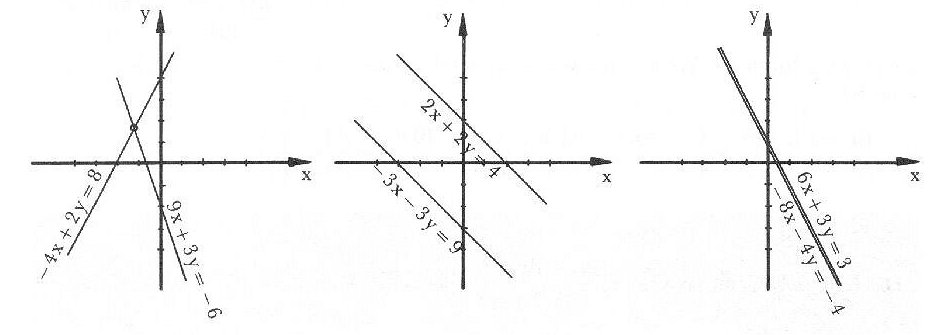
\includegraphics[width=\textwidth]{2te/linearegleichungssysteme/bilder/3arten.jpg}

\bme Falls das Gleichungssystem eindeutig l\"{o}sbar ist, erhalten wir die L\"{o}sung als Schnittpunkt der $2$
Geraden! \eme

\bb "`Normalfall"': L�se das Gleichungssystem graphisch.  $ \left\{ \begin{array}{rcl} 4x+3y & = & 17 \\
                                               -6x+8y & = & 12
                                       \end{array} \right.        $ \eb


\ba \bn \item L\"{o}se die folgenden Gleichungssysteme auf graphischem Wege. Mache jedes Mal die Probe:

\bt{llll}
 a) & $  \left\{ \begin{array}{rcl}  3x + y& = & -2 \\
                                              x+2y & = & 3
                                       \end{array} \right.       $      &  b) & $  \left\{ \begin{array}{rcl} 2x-6y & = & -3 \\
                                               3x+4y & = & 15
                                       \end{array} \right.       $ \et





\item  Bei den wenigsten Systemen wird es m\"{o}glich sein, die L\"{o}sung auf graphischem Wege exakt zu erhalten, weil
die gesuchten Zahlen in der Regel weder ganz noch einfache Br\"{u}che sind. Das folgende System ist von der
erw\"{a}hnten Art. Bestimme die L\"{o}sung graphisch so genau wie m\"{o}glich und mache die Probe:

\begin{displaymath} \left\{ \begin{array}{rcl} 2x + 3y & = & 6 \\
                                               -x + 2y & = & 2
                                       \end{array} \right. \end{displaymath}


\item  Die L\"{o}sung des Systems $x = 3$ und $y = 2$ kann zwar unmittelbar abgelesen werden. Trotzdem ist es von
Interesse, diese L\"{o}sung graphisch als Schnittpunkt zweier Geraden zu interpretieren. Zeichne diese Geraden.

\item Ob ein Gleichungssystem mit zwei Gleichungen und zwei Variablen genau eine L\"{o}sung hat, kann man ganz
einfach anhand der Steigungen der den Gleichungen entsprechenden Geraden nachpr\"{u}fen: Die Steigungen m\"{u}ssen
$\dots $sein. \en \ea

\section{Rechnerische L\"{o}sungsverfahren}

Die Schw\"{a}chen der graphischen L\"{o}sungsmethode liegen auf der Hand: nur selten erhalten wir eine exakte L\"{o}sung,
meistens handelt es sich um N\"{a}herungswerte. Um die L\"{o}sungen exakt zu bestimmen, ben\"{o}tigen wir also andere
Methoden:

\bn \item Das Gleichsetzungsverfahren
\item Das Einsetzungsverfahren
\item Das Additionsverfahren
\item Das Determinantenverfahren
\en


\subsection{Das Gleichsetzungsverfahren:}

\bb  $ \left\{ \begin{array}{rcl} y & = & \frac{1}{3}x \\
                                               y & = & \frac{3}{5}x+\frac{1}{10}
                                       \end{array} \right.        $ \eb



\bme {\bf Gleichsetzungsverfahren}

\bn \item L\"{o}se beide Gleichungen nach derselben Variablen auf \item  Setze die anderen Seiten gleich (daher
der Name!) und l\"{o}se diese Gleichung.

\item \bn \item Wenn du ein Ergebnis f\"{u}r eine Unbekannte erh\"{a}ltst, setze es in eine der beiden ersten Gleichungen ein
und bestimme somit den fehlenden Wert. \item Erh\"{a}ltst du einen Widerspruch, also eine Gleichung der Art $a =
b$, so gibt es keine L\"{o}sung: $L = \{ \}$

 Erh\"{a}ltst du eine Gleichung der Art $a = a$, so erh\"{a}ltst du unendlich viele L\"{o}sungen, genau alle Zahlenpaare,
welche eine der beiden Gleichungen erf\"{u}llen. \en

\item  Wenn du ein L\"{o}sungspaar erh\"{a}ltst, so mache die Probe, indem du in beide Gleichungen deine errechneten
Werte einsetzt. \en \eme



\ba  L\"{o}se die folg. Systeme nach dem Gleichssetzungsverfahren. Mache jedes Mal die Probe. Denke wieder einmal
daran: Bei Umformungen jeglicher Art, speziell auch beim L\"{o}sen von Gleichungen und Gleichungssystemen: Sauber
und \"{u}bersichtlich darstellen. Dies wird sich immer wieder lohnen.

\bt{llllll}
 a) & $ \left\{ \begin{array}{rcl} y & = & 3x-17 \\
                                               y & = & 2x-10
                                       \end{array} \right.        $      &  b) & $   \left\{ \begin{array}{rcl} y & = & -2x+3 \\
                                               y & = & -2x+2
                                       \end{array} \right.       $    &  c) & $ \left\{ \begin{array}{rcl} 5y-x & = & 33 \\
                                               5y-x & = & 11
                                       \end{array} \right.         $ \et

\ea

\subsection{Das Einsetzungsverfahren:}

\bb  $ \left\{ \begin{array}{rcl} y & = & 2x+4 \\
                                               9x+3y & = & -6
                                       \end{array} \right.        $ \eb

Sind die $2$ Gleichungen nicht so bequem nach einer Variablen aufgel\"{o}st, so hilft dieses Vorgehen oft weiter:

\bme {\bf Einsetzungsverfahren}

\bn \item  Setze aus der Gleichung, die nach einer Variablen aufgel\"{o}st ist, diese in die andere Gleichung
ein.

\item L\"{o}se die so entstandene Gleichung.

\bn \item  Wenn du ein Ergebnis f\"{u}r eine Unbekannte erh\"{a}ltst, setze es in eine der beiden ersten Gleichungen
ein und bestimme somit den fehlenden Wert.

 \item  Erh\"{a}ltst du einen Widerspruch, also eine Gleichung der Art $a = b$, so
gibt es keine L\"{o}sung: $L = \{ \}$

\item  Erh\"{a}ltst du eine Gleichung der Art $a = a$, so erh\"{a}ltst du unendlich viele L\"{o}sungen, genau alle
Zahlenpaare, welche eine der beiden Gleichungen erf\"{u}llen. \en

\item  Wenn du ein L\"{o}sungspaar erh\"{a}ltst, so mache die Probe, indem du in beide Gleichungen deine
errechneten Werte einsetzt. \en \eme

\ba  L\"{o}se die folg. Systeme nach dem Einsetzungsverfahren.

\bt{llllll}
 a) & $  \left\{ \begin{array}{rcl} 3x-4y & = & 7 \\
                                    x+2y & = & 19
                                       \end{array} \right.$
 &  b) & $\left\{ \begin{array}{rcl} 12x+2y & = & 5 \\
                                     11x+y & = & 12\end{array} \right.$
 c) & $ \left\{ \begin{array}{rcl} 3x_1+7x_2 & = & 15 \\
                                   6x_1-5x_2 & = & -27
                                       \end{array} \right.        $ \\
 d) & $  \left\{ \begin{array}{rcl} 2u+3v & = & 7 \\
                                    v & =  & \frac{1}{2}u+1
                                       \end{array} \right.      $      &
 e) & $   \left\{ \begin{array}{rcl} 4x-7y & = & -3 \\
                                     x+2 & = & 0
                                       \end{array} \right.      $ \et
\ea


 \subsection{Das Additionsverfahren:}

Hat das Gleichungssystem nicht schon eine besondere Form, die f\"{u}r das Gleichsetzungs- bzw.
Einsetzungsverfahren geeignet ist, so bietet sich das Additionsverfahren an. Es ist im ersten Moment
vielleicht die komplizierteste Methode, doch nach einiger \"{U}bung sehr effizient und vor allem auch bei gr\"{o}{\ss}ere
Gleichungssysteme (mehrere Gleichungen und mehrere Unbekannte) den anderen M\"{o}glichkeiten \"{u}berlegen.





\bme \bn \item  Multipliziere die erste oder (und) zweite Gleichung mit einer Zahl, so dass bei einer der
zwei Variablen die Koeffizienten jeweils die Gegenzahlen sind (z.B. $5x$ in der 1. Gleichung und $-5x$ in der
2.)

\item  Addiere die linken und die rechten Seiten beider Gleichungen, so f\"{a}llt eine Variable weg und du erh\"{a}ltst
eine Gleichung mit einer Unbekannten, die du wieder l\"{o}sen kannst.

\item Setze den so erhaltenen Wert in eine der beiden Ausgangsgleichungen ein und errechne dadurch den Wert
der zweiten Unbekannten.

\item  Mach die Probe.
\en \eme



\ba \bn \item  L\"{o}se die folgenden Systeme mit der Additionsmethode:


\bt{llll}
 a) & $    \left\{ \begin{array}{rcl}    3x +7y    & = &  9           \\
                                5x-4y    & = &   2          \end{array} \right.    $      &
  b) & $  \left\{ \begin{array}{rcl}      10x+8y & = & 9            \\
                                         7x+5y & = -20&             \end{array} \right.       $ \\
 c) & $     \left\{ \begin{array}{rcl}  4x-25y   & = & 15            \\
                                         2x+15y  & = &  3           \end{array} \right.   $      &
 d) & $ \left\{ \begin{array}{rcl}    26x+33y     & = & -11            \\
                                      39x+55y     & = &    -19         \end{array} \right.        $ \et




\item  F\"{u}r das Gleichungssystem $ \left\{ \begin{array}{rcl} x-2y   & = & 4         \\
                                      4x+3y     & = &    9         \end{array} \right.$
erh\"{a}lt man \bn \item graphisch die N\"{a}herungsl\"{o}sung $\dots$. \item mit dem Einsetzungsverfahren die exakte
L\"{o}sung $\dots$ \item mit dem Additionsverfahren $\dots$ \item  Vergleiche die Resultate! \en \en \ea

\subsection{Das Determinantenverfahren:}

 \bd  Unter der  Koeffizientenmatrix (oder kurz {\bf Matrix}) eines linearen Gleichungssystems
 \begin{displaymath} %\left{
       \begin{array}{rcl}
          a_{11}x_1+a_{12}x_2&=&b_1\\
          a_{21}x_1+a_{22}x_2&=&b_2
       \end{array} %\right
   \end{displaymath}
   versteht man die Tabelle der Koeffizienten (in runden
   Klammern):
\[   \begin{pmatrix}
    a_{11} & a_{12} \\
    a_{21} & a_{22}
  \end{pmatrix}\]
\ed  
\bb  
Bestimme die Koeffizientenmatrix: \begin{displaymath}
       \begin{array}{rcl}
          3x-2y&=&5\\
          -7x+8y&=&-1
       \end{array}
   \end{displaymath}
\eb  

 \bd 
Unter der {\bf Determinante ($\det$)} einer Matrix
\[  M=  \begin{pmatrix}
    a_{11} & a_{12} \\
    a_{21} & a_{22}
  \end{pmatrix}\]
versteht man die Zahl $D=a_{11}\cdot a_{22}- a_{12}\cdot a_{21}$.
  \ed  
\subsubsection*{Merkregel}
Zur Berechnung der Determinante einer Matrix merke man sich: Produkt der Hauptdiagonale minus Produkt der
Nebendiagonale.

\noindent Man schreibt:

\begin{displaymath}
 \det(M)=  \left|
          \begin{array}{cc}
            a_{11} & a_{12} \\
            a_{21} & a_{22}
          \end{array}
          \right|= a_{11}\cdot a_{22}- a_{12}\cdot a_{21}
          \end{displaymath}


\bb  
Berechne die Determinante von $   \begin{pmatrix}
    3 & -2 \\
    1 & -4
  \end{pmatrix} $.
\eb  
\ba 
\begin{enumerate}
\item Berechne die folgenden Determinanten:
  \begin{enumerate}
  \item   \begin{displaymath}
          \left|
          \begin{array}{cc}
            2 & 8 \\
            9 & 10
          \end{array}
          \right|
          \end{displaymath}

  \item   \begin{displaymath}
          \left|
          \begin{array}{cc}
            -3 & 6 \\
            -9 & 7
          \end{array}
          \right|
          \end{displaymath}
  \end{enumerate}

\item Vereinfache so weit als m\"{o}glich:
  \begin{enumerate}
  \item   \begin{displaymath}
          \left|
          \begin{array}{cc}
            2c & 3d\\
            4c & 5d
          \end{array}
          \right|
          \end{displaymath}

  \item   \begin{displaymath}
          \left|
          \begin{array}{cc}
            a+b & a-b \\
            a-2b & a+2b
          \end{array}
          \right|
          \end{displaymath}
  \end{enumerate}
\end{enumerate}
\ea 
  \bs Ein lineares Gleichungssystem ist genau dann eindeutig l\"{o}sbar, wenn die Determinante der Koeffizientenmatrix
nicht Null ist:
  \begin{displaymath}
       \begin{array}{rcl}
          a_{11}x_1+a_{12}x_2&=&b_1\\
          a_{21}x_1+a_{22}x_2&=&b_2
       \end{array}  \; \mbox{l\"{o}sbar} \Leftrightarrow
\left|
          \begin{array}{cc}
            a_{11} & a_{12} \\
            a_{21} & a_{22}
          \end{array}
          \right|= a_{11}\cdot a_{22}- a_{12}\cdot a_{21}       \neq 0
   \end{displaymath}
  \es 

\ba 
\begin{enumerate}
\item Ist das Gleichungssystem
    \begin{displaymath}
       \left\{
       \begin{array}{l}
          3x-2y=9\\
          6x-4y=17
       \end{array}
       \right.
   \end{displaymath} l\"{o}sbar?

\item Ein Gleichungssystem habe die Koeffizientenmatrix
 \begin{displaymath}
       M= \left(
       \begin{array}{cc}
          1  &  1  \\
          a  &  b
       \end{array}
       \right).
   \end{displaymath}
   Welche Bedingung muss erf\"{u}llt sein, damit das Gleichungssystem l\"{o}sbar ist?
\end{enumerate}
\ea 
 \bd 
Ersetzt man die erste bzw. zweite Spalte einer Koeffizientenmatrix $  M=  \begin{pmatrix}
    a_{11} & a_{12} \\
    a_{21} & a_{22}
  \end{pmatrix}$ durch die Spalte $
  \begin{pmatrix}
     b_1 \\
     b_2
  \end{pmatrix}   $ des Gleichungssystems
 $       \begin{array}{rcl}
          a_{11}x_1+a_{12}x_2&=&b_1\\
          a_{21}x_1+a_{22}x_2&=&b_2
       \end{array}$, so erh\"{a}lt man die Matrizen:
 \[  \begin{pmatrix}
    b_{1} & a_{12} \\
    b_{2} & a_{22}
  \end{pmatrix} \qquad  \begin{pmatrix}
    a_{11} & b_{1} \\
    a_{21} & b_{2}
  \end{pmatrix}\]
Mit $D_1$ bzw. $D_2$ werden nun die Determinanten dieser 2 Matrizen bezeichnet, also:
\[D_1 = \left|
          \begin{array}{cc}
            b_{1} & a_{12} \\
            b_{2} & a_{22}
          \end{array}
          \right| \qquad
          D_2 = \left|
          \begin{array}{cc}
            a_{11} & a_{12} \\
            a_{21} & a_{22}
          \end{array}
          \right|\]
  \ed  
  \bs {\bf Cramersche Regel}

Vorausgesetzt dass das lineare Gleichungssystem genau eine L\"{o}sung $(x_1|x_2)$ hat, kann diese wie folgt
berechnet werden:
\[x_1=\frac{D_1}{D} \qquad x_2=\frac{D_2}{D}\]
  \es 

\ba Beweise die Cramersche Regel fr $2 \times 2$ Matrizen.\ea


\bb  
 \begin{displaymath}
       \left\{
       \begin{array}{l}
          2x_1-x_2=5\\
          -x_1+4x_2=1
       \end{array}
       \right.
   \end{displaymath}
\eb  
\ba 
 Bestimme die L\"{o}sungsmenge der folg. Gleichungssysteme mit Hilfe
      der Cramerschen Regel:
  \begin{enumerate}
  \item       \begin{displaymath}
       \left\{
       \begin{array}{l}
          13x-7y=2\\
          5x+3y=4
       \end{array}
       \right.
   \end{displaymath}

  \item       \begin{displaymath}
       \left\{
       \begin{array}{l}
          3y=6\\
          5x-4y=8
       \end{array}
       \right.
   \end{displaymath}
  \end{enumerate}
\ea 





\section{Textaufgaben}

\ba
\bn \item Vergr��ert man die L�nge eines Rechtecks um $2$cm und verkleinert die Breite um $1$cm, dann bleibt der Fl�cheninhalt unver�ndert. Verkleinert man die L�nge um $1$cm und vergr��ert man die Breite um $2$cm, dann nimmt der Fl�cheninhalt um $12$cm$^2$ zu. Berechne die L�nge und die Breite des Rechtecks.


%\item In der Kneipe (siehe Abb. \ref{kneipejpg} auf Seite \pageref{kneipejpg}).

%\begin{figure}[hbt]
%\begin{center} \label{kneipejpg}
%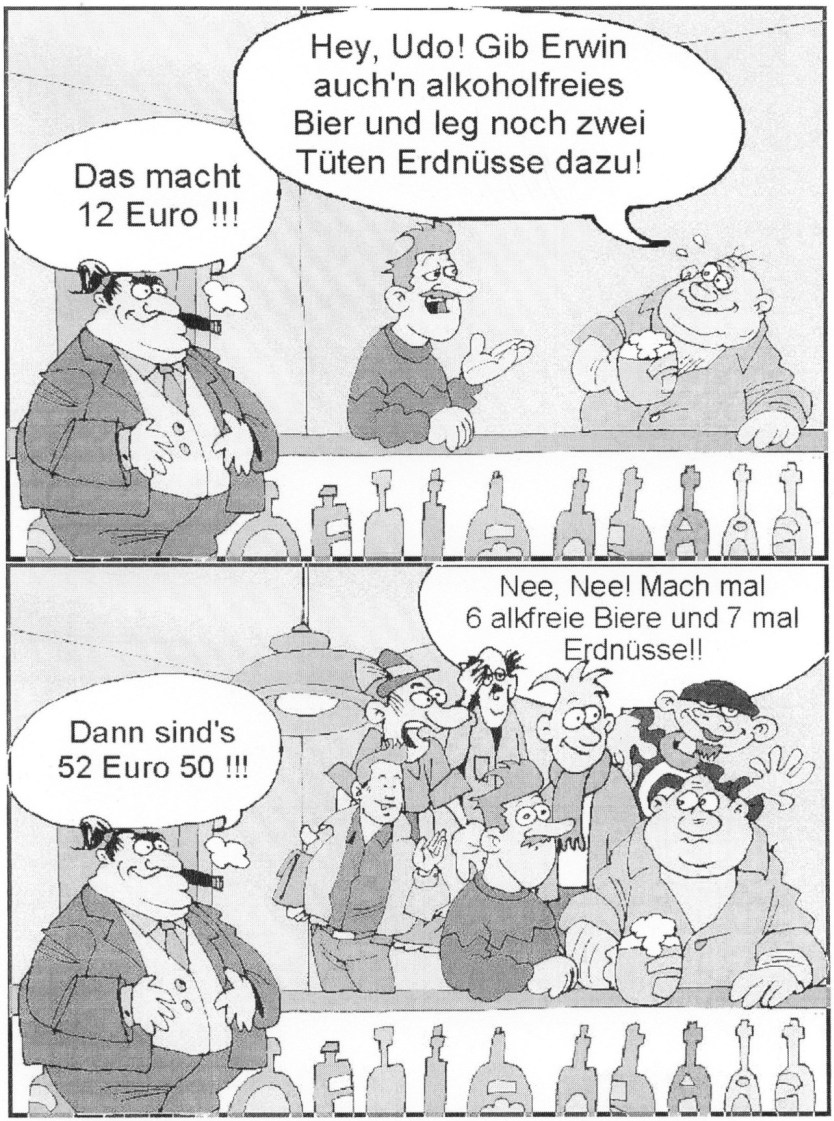
\includegraphics[width=8cm]{2te/linearegleichungssysteme/bilder/kneipe.jpg}
%\caption{In der Kneipe}
%\end{center}
%\end{figure}



\item Der noch sehr r�stige Vater sagt zu seinem Sohn: "`In elf Jahren bin ich genau doppelt so alt wie du vor elf Jahren warst."' Darauf antwortet der Sohn: "`Aber vor elf Jahren warst du nur $\frac87$ mal so alt wie ich in elf Jahren sein werde."' Wie alt sind die beiden?

\item "`Geben sie mir drei Kilo �pfel und vier Kilo Birnen"', sagt Susi und legt $26$ Euro auf den Ladentisch, genau den richtigen Betrag. Als der Ladenbesitzer das Obst einpacken will, ruft Susi: "`Geben sie mir doch lieber $4$ Kilo �pfel und $3$ Kilo Birnen."' "`Dann bekommst du $90$ Cent zurck"', sagt daraufhin der Ladenbesitzer. Was kostet das Obst?

\item Ein Textilgesch�ft bezieht $200$ Hemden und $250$ Pullover, die laut Rechnung zusammen $24.500$ Euro kosten. Die Hemden werden mit $20\%$, die Pullover mit $40\%$ Aufschlag verkauft. Dabei werden insgesamt $31.900$ Euro eingenommen. Wie teuer waren ein Hemd bzw. ein Pullover im Einkauf?

\item Bauer Franz h�lt auf seinem Hof nur Schweine und H�hner, insgesamt $100$ Tiere. Irgendwann hat er festgestellt, dass diese insgesamt $268$ Beine haben. Wie viele Schweine und wie viele H�hner hat Franz?


\item Magie der M�nzen:

\begin{center}
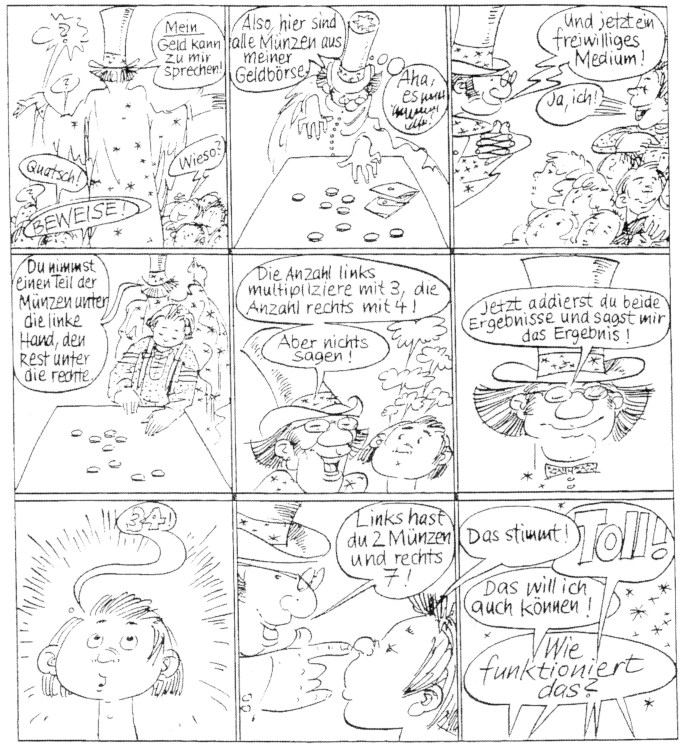
\includegraphics[width=9cm]{2te/linearegleichungssysteme/bilder/zauberer.jpg}
\end{center} 



\item Eulers Aufgabe

Aus dem Buch "`Vollst�ndige Anleitung zur Algebra"' von Leonhard Euler (1707-1783):

{\it "`Zwei Personen sind $29$ Rubel schuldig; nun hat zwar jeder Geld, doch nicht so viel, dass er diese gemeinschaftliche Schuld allein bezahlen k�nnte; drum sagt der Erste zum anderen: Gibst du mir zwei Drittel deines Geldes, so kann ich die Schuld sogleich allein bezahlen. Der andere antwortet dagegen: Gibst du mir drei Viertel deines Geldes, so kann ich die Schuld allein bezahlen."'}

Wie viel Geld hat jeder?






\item Dreiecke mit verschl�sselten Ma�angaben

Acht Dreiecke verraten so viel von ihren Ma�en, dass man sie konstruieren kann. Allerdings haben sie ihre Angaben ein wenig verschl�sselt. - Berechne die Ma�e und konstruiere dann die Dreiecke.

�brigens: Eins der Dreiecke hat sich wohl geirrt. Mit seinen Ma�en ist beim besten Willen kein Dreieck zu konstruieren. Welches Dreieck ist es?

\begin{description}
\item[Dreieck 1:] Die Seite $c$ ist $8$cm lang. $a$ und $b$ sind zusammen $10$cm lang, $b$ ist $3$cm gr��er als $a$.

\item[Dreieck 2:] Die H�he $h_c$ und die Seite $a$ sind gleich lang, und zwar $4$cm. Die vierfache L�nge von $b$  ist gleich der siebenfachen L�nge von $a$.

\item[Dreieck 3:] Es gilt: $a<b<c$. Je zwei Seiten unterscheiden sich jeweils um $3$cm oder um $6$cm. $a$ ist halb so gro� wie $c$.

\item[Dreieck 4:] Der Umfang betr�gt $20$cm. $c$ ist $4$cm l�nger als $b$. Die dreifache L�nge von $b$ ist um $2$cm l�nger als die doppelte L�nge von $c$.

\item[Dreieck 5:] Die Winkel $\alpha$ und $\beta$ sind gleich gro�. Die doppelte L�nge von $a$ ist die dreifache L�nge von $c$. Der Umfang des Dreiecks betr�gt $1$cm.

\item[Dreieck 6:] Der Winkel $\alpha$ betr�gt $60$. Die sechsfache L�nge von $h_c$ ist die dreifache L�nge von $c$. Die Differenz von $h_c$ und $c$ betr�gt $4$cm.

\item[Dreieck 7:] $a$ und $b$ sind zusammen $21$cm lang. Die L�nge von $b$ betr�gt $75\%$ der L�nge von $a$. $c^2$ ist um $1$ gr��er als das Vierfache von $a$.

\item[Dreieck 8:] Der Umfang des Dreiecks betr�gt $12$cm. Die L�nge von $c$ betr�gt $80\%$ der L�nge von $b$. $a$ und $b$ zusammen sind doppelt so lang wie $c$.
\end{description}
\en
\ea

\section{3x3 Gleichungssysteme} 


Abschlie{\ss}end gehen wir noch kurz auf lineare Gleichungssysteme
mit 3 Gleichungen und 3 Unbekannten ein. Alle rechnerischen Verfahren bleiben auch hier g�ltig. Von Vorteil sind dabei saubere Heftf�hrung, einen guten �berblick und nat�rlich Rechensicherheit.

Das zeichnerische Verfahren ist aber nicht mehr geeignet, man m�sste auf ein Papier (2-Dimensionen) in einem drei-dimensionalen-Koordinatensystem den Schnittpunkt von 3 Ebenen ermitteln. 

\bb Bestimme die L\"{o}sungsmenge:
$ \left\{ \begin{array}{rcl}    5x-6y+4z    & = & 27            \\
                                     -10x+3y+2z   & = &    -69  \\
                                     15x+9y+10z & = & 210           \end{array} \right.        $
\eb

\ba \bn \item Bestimme die L\"{o}sungsmenge:

$ \left\{ \begin{array}{rcl}    5x-6y+4z    & = & 27            \\
                                     -10x+3y+2z   & = &    -69  \\
                                     15x+9y+10z & = & 210           \end{array} \right.        $


\item Wie lang sind die Seiten eines Dreiecks, wenn die Summen von jeweils $2$ Seiten $22$cm, $23$cm und $25$cm
betragen?  

\item Sdtirol ist ein bekanntes Obstanbaugebiet. Irgendwo befindet sich eine kleine Fabrik, die aus dem angebauten Obst drei Sorten von Produkten herstellt: Obstsalat, Multivitaminsaft und Marmelade.

In der Hauptsaison sollen aus �pfeln, Birnen und Kirschen pro Monat $100$kg Obstsalat, $500$l Saft ($1$l $\cong$ $1$kg) und $200$kg Marmelade hergestellt werden. F�r den Obstsalat werden zu gleichen Anteilen �pfel, Birnen und Kirschen verwendet. Pro Liter Multivitaminsaft werden an Gewicht dreimal so viele �pfel wie Kirschen und doppelt so viele Birnen wie Kirschen verwendet. F�r die Herstellung der Marmelade kommen auf ein Kilogramm jeweils gleich viele �pfel und Birnen.

Welche Fruchtmengen sind f�r die Herstellung dieser Produkte erforderlich?\en \ea


\subsection{Determinatenverfahren:}
  \bs {\bf Regel von
Sarrus\footnote{nach {\it P.F. Sarrus} (1798-1861)}}

Die Determinante einer $3 \times 3$-Matrix M kann durch die Formel:
\[\begin{array}{rcl}
    \det(M)&=&a_{11}a_{22}a_{33}+a_{12}a_{23}a_{31}+a_{13}a_{21}a_{32}\\
           & &-a_{13}a_{22}a_{31}-a_{11}a_{23}a_{32}-a_{12}a_{21}a_{33}
\end{array}\]
  \es 
\subsubsection{Merkregel: Regel von Sarrus}
\[\begin{array}{ccccc}
  a_{11} & a_{12} & a_{13} & a_{11} & a_{12} \\
  a_{21} & a_{22} & a_{23} & a_{21} & a_{22} \\
  a_{31} & a_{32} & a_{33} & a_{31} & a_{32}
  \end{array}\]
\bb  
Berechne:
\begin{displaymath}
 \det(M)=  \left|
          \begin{array}{ccc}
            1&0&-1\\
            2&1&1\\
            1&-3&2  \end{array}
          \right|
          \end{displaymath}
\eb  
\ba 
\begin{enumerate}
\item Sind die folgenden Gleichungssysteme l\"{o}sbar? \label{aufoha}
    \begin{enumerate}
 \item
    \begin{displaymath}
       \left\{
       \begin{array}{l}
          x_1+x_2+x_3=3\\
          x_1-x_2+x_3=1\\
          x_1+x_3=2
       \end{array}
       \right.
   \end{displaymath}
 \item
    \begin{displaymath}
       \left\{
       \begin{array}{l}
          -3x_1+2x_2-x_3=8\\
          4x_2-6x_3=16\\
          -x_1+x_2-x_3=5
       \end{array}
       \right.
   \end{displaymath}
\end{enumerate}

\hfill (L\"{o}sung: a.) unl\"{o}sbar, b.) l\"{o}sbar)

\item Warum ist das folgende Gleichungssystem nicht eindeutig l\"{o}sbar?
    \begin{displaymath}
       \left\{
       \begin{array}{l}
          2x_1+2x_3=1\\
          x_1-x_2=0\\
          -x_1+x_2=1
       \end{array}
       \right.
    \end{displaymath}
\end{enumerate}
\ea 

Demnach k\"{o}nnen jetzt Gleichungssysteme mit 3 Gleichungen und 3 Unbekannte sehr einfach gel\"{o}st werden: Man
berechne sich die Determinanten $D$, $D_1$, $D_2$ und $D_3$ mit Hilfe der {\it Regel von Sarrus} und wende
dann die {\it Cramer'sche Regel} an. Dazu folgendes Beispiel.
\bb        \begin{displaymath}
       \left\{
       \begin{array}{l}
       5x+11y-21z=0\\
       7x-2y-7z=5\\
       3x-8y+14z=12       \end{array}
       \right.
   \end{displaymath}
\eb  

\ba \bn \item Formuliere die Cramersche Regel f�r ein 3x3 Gleichungssystem.
\item Beweise die Cramersche Regel f�r ein 3x3 Gleichungssystem (schwer!)
\en \ea




\ba 
\begin{enumerate}
\item Berechne die L\"{o}sungsmenge der l\"{o}sbaren Gleichungssysteme aus Aufgabe
        \ref{aufoha} mit der "`Regel von Sarrus"'.

\hfill (L\"{o}sung: $\mathbb{L}=\{(-4; -5; -6)\})$

\item Bevor du das folgende Gleichungssystem l\"{o}st, solltest du die Gleichungen
      vereinfachen und dadurch das GS auf Normalform bringen.
    \begin{displaymath}
       \left\{
       \begin{array}{l}
          \frac{x_1}{2}+\frac{2(2x_2-1)}{5}-\frac{x_3}{4}=4\\
          \frac{7x_2}{6}+\frac{4(x_1-1)}{3}-\frac{x_3}{2}=\frac{25}{6}\\
          x_1+x_2+x_3=1
       \end{array}
       \right.
   \end{displaymath}

\hfill (L\"{o}sung: $\mathbb{L}=\{(2; 3; -4)\})$

\item Oberstrebi soll drei Zahlen ermitteln. Er erh\"{a}lt als Hinweise die
      drei Summen aus jeweils zwei dieser drei Zahlen. Die Summen lauten
      9, 20 und 21. Wie hei{\ss}en die drei gesuchten Zahlen?

\hfill (L\"{o}sung: die gesuchten Zahlen hei{\ss}en: 4, 5 und 16)

\item Die Seilbahn Meran2000 verlangt f\"{u}r Berg-und Talfahrt zusammen 12 \euro , f\"{u}r die Bergfahrt allein 9\, \euro \, und f\"{u}r die Talfahrt allein
      6 \euro . An einem sch\"{o}nen Sommertag (schulfrei!) fuhren im ganzen
      680 Personen hinauf und 520 hinab. Dabei gingen 7.860 \euro ein.
      Wie viele Tickets jeder Art sind gel\"{o}st worden?

\hfill (L\"{o}sung: Berg+Tal: 460, Berg: 220, Tal: 60)








% 3x3
\item {\bf Mathematik - Olympiade Biennium}

Ad una gara matematica partecipano $1200$ candidati. Il $40\%$ di essi riceve una medaglia (d'oro, d'argento o di bronzo). Il numero di medaglie di bronzo \'e triplo di quello di medaglie d'oro; il numero di medaglie d'argento \'e doppio di quello di medaglie d'oro. Quante sono le medaglie d'argento?

(A)	120, (B) 144, (C) 160, (D) 180, (E) nessuna delle precedenti.
\end{enumerate}
\ea 

\section{\"{U}bungen zur  Schularbeit: Lineare Gleichungssysteme}

\ba
\bn
\item Denk dir selbst ein lineares Gleichungssystem mit zwei Variablen aus, das die L�sungsmenge $\mathbb{L}={-2;5}$ hat und sich besonders gut
\bn \item mit dem Einsetzungsverfahren \item mit dem Additionsverfahren\en l�sen l�sst.




\item Gleichungssysteme aufstellen;



\begin{center} 
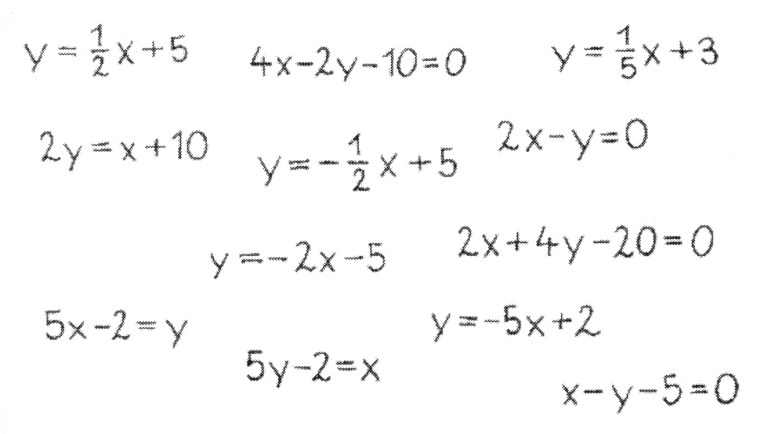
\includegraphics[width=8cm]{2te/linearegleichungssysteme/bilder/gleichungen.jpg}
%\caption{Gleichungen}\label{gleichungssystemejpg}
\end{center}


Bilde aus den vorgegebenen Gleichungen jeweils zwei Gleichungssysteme mir einer L�sung, mit keiner L�sung und unendlich vielen L�sungen.





\item  Der neueste Kinostreifen ist ein voller Erfolg f\"{u}r den Kinobesitzer, welcher $444$ \euro \, f\"{u}r die
 ausverkaufte Abendvorstellung kassierte. Wie viele Erwachsenen sahen den Film und wie viele
Jugendliche, wenn Erwachsene $6$ \euro \, und Jugendliche $5$ \euro \, bezahlen und insgesamt $80$ Personen
im Kino Platz finden?

\item  In einer Buchhandlung werden $2$ Sorten Taschenb\"{u}cher im Sonderangebot verkauft. Lisi kauft $4$ B\"{u}cher von
der 1. Sorte und bringt $3$ B\"{u}cher der 2. Sorte als Umtausch zur\"{u}ck (bekommt den entsprechenden Betrag!). Sie
bezahlt an der Kasse $2$ \euro. Peter kauft 2 B\"{u}cher der 1. und 2 B\"{u}cher der 2. Sorte und bezahlt an der
Kasse $4,5$ \euro. Was kostet je ein Buch von jeder Sorte?

\item  Wie lautet die lineare Funktion, deren Graph durch die Punkte P=$(4/-2)$ und Q=$(-2/-5)$ verl\"{a}uft?

\item  Bestimme den Schnittpunkt des Gleichungssystems
$\left\{ \begin{array}{rcl} 5x + 2y    & = & 16            \\
                                     16x + 7y  & = & 10           \end{array} \right.$
\bn \item graphisch \item  rechnerisch. \en

\item Gib zur Gleichung $x + 2y = -8$ eine 2. Gleichung an, so dass das System \bn \item keine L\"{o}sung hat. \item unendlich viele L\"{o}sungen hat.\en

\item Die Summe zweier Zahlen betr\"{a}gt $15$, ihre Differenz $-1$. Erstelle ein lineares Gleichungssystem
und l\"{o}se es mit einer Methode deiner Wahl. 





\item {\bf Mathematik Olimpiade 2003 - Biennium:}

\bn \item 
Un gelataio prepara $20$ kg di gelato e lo rivende nel corso della giornata in coni
piccoli da $1,20$ Euro di due palline e coni grandi da $1,60$ Euro di tre palline. Da ogni
kg di gelato ha ricavato $12$ palline; alla fine della giornata, ha incassato in totale
$137,60$ Euro. Quanti coni grandi ha venduto?

(A) 17 (B) 24 (C) 32 (D) 43 (E) 50.

\item  Un venditore di palloncini ha a disposizione due bombole di elio uguali e dei palloncini
piccoli e grandi. Utilizza tutta la prima bombola per gonfiare 80 palloncini
piccoli, tutti alla stessa pressione. Considerato che da gonfi i palloncini grandi
hanno la stessa forma e la stessa pressione dei piccoli, ma una superficie 4 volte pi\'u
grande, quanti palloncini grandi pu\'u riempire con la seconda bombola?

(A) 10 (B) 16 (C) 20 (D) 24 (E) 40.

\en\en
\ea
 \chapter{Funktionen} 

Jedem von euch sollte in der Zwischenzeit bewusst geworden sein, dass es in der Mathematik sehr viel um
Gleichungen geht. Der Begriff der Gleichung ist und wird auch f\"{u}r die n\"{a}chsten Jahre (zumindest im
Mathematikunterricht) ein zentraler Begriff bleiben. Neben dem Begriff der Gleichung existiert ein weiterer
sehr wichtiger Begriff und  zwar die Funktionen.

In diesem Abschnitt gibt es die erste Einf�hrung;  wichtig ist nun sich mit diesem Kapitel sehr gut vertraut
zu machen, denn die enorme Bedeutung kann hier gar nicht zum Ausdruck gebracht werden.


\subsection*{Wozu sind Funktionen gut?}





Immer dann, wenn der Wert einer Gr��e vom Wert einer anderen Gr��e {\it abh�ngt}, liegt eine Funktion vor. Da die Natur und unser Leben voll von solchen Abh�ngigkeiten sind, kann eine unermesslich gro�e Anzahl von Vorg�ngen und Zusammenh�ngen in der mathematischen Sprache der Funktionen beschrieben, modelliert und verstanden werden - manchmal sehr genau, in Form ausgefeilter Theorien, manchmal nur in grober N�herung. 

Betrachte  etwa ein Thermometer, das an irgendeinem Ort h�ngt. Die von ihm angezeigte Temperatur wird nicht immer dieselbe sein, sondern sich mit der Zeit �ndern, z.B. tages- oder jahreszeitlichen Schwankungen unterworfen sein. Mit anderen Worten, die Temperatur {\it h�ngt} vom Zeitpunkt {\it ab}, an dem sie gemessen wird. Dies stellt  eine Funktion dar: Zu jedem gegebenen Zeitpunkt $t$ (Eingabe) wird eine bestimmte Temperatur $T$ (Ausgabe) angezeigt. Man sagt, die Temperatur "`ist eine Funktion der Zeit"'.




\section{Beispiele und Definition}

\bb
\begin{enumerate}
\item In einem Schaufenster unter den Lauben sind alle ausgestellten Artikel mit einem Preisschild versehen.
Bei keinem Artikel fehlt das Schild, es gibt aber Artikel die
gleich viel Kosten.

Abstrakt betrachtet handelt es sich hierbei um zwei Mengen: $A=$
Menge der Waren, $B=$ Menge der Preise. Dabei wird jedem Artikel
ein Preis {\it zugeordnet}; also jedem Element $x\in A$ genau ein
Element $y\in B$.

\item Deine Familie besteht aus einer gewissen Anzahl von
Familienmitgliedern. Nun wird jedem Familienmitglied seine
Blutgruppe zugeordnet.

Es handelt sich also hierbei wieder um eine Zuordnung zwischen
zweier Mengen (vgl. Abb. \ref{-1}), und zwar:

$A=$ \qquad \qquad   $B=$



\item Unter dem {\bf Betrag} einer Zahl versteht man ihren Abstand
zum Nullpunkt auf dem Zahlenstrahl. So hat die Zahl 5 den Betrag 5
und die Zahl -9 den Betrag 9. \label{7}

Man kann sich also merken: der Betrag einer Zahl ordnet einer positiven Zahl dieselbe Zahl zu, bei einer
negativen Zahl wird das "`Vorzeichen weggelassen"'.

Die Schreibweise: $|5|=5$ und $|-9|=9$.

Hierbei handelt es sich also um eine Zuordnung zwischen
Zahlenmengen.


\end{enumerate}
\eb

Diese Beispiele haben gemeinsam, dass jeweils allen Elementen einer Menge genau ein Element einer weiteren
Menge zugeordnet wird. Dies f\"{u}hrt auf die folgende Definition:

\bd
Gegeben sind zwei Mengen: die Definitionsmenge $D$ und die Wertemenge $W$. Unter einer {\bf Funktion} $f$
versteht man eine {\it Zuordnung}. Dabei muss {\it jedem} Element $x$ aus dem Definitionsbereich  {\it genau
ein} Element $y$ aus dem Wertebereich zugeordnet werden.

Man schreibt daf\"{u}r:

\[\begin{array}{rrcl}
  f: & D & \rightarrow & W \\
   & x & \mapsto & y
\end{array}\]
\ed



\begin{Bem}
\begin{enumerate}
\item
Dem $x$ aus der Definitionsmenge ($x \in D$) wird durch die Funktion $f$ {\it genau ein}  Element aus der
Wertemenge ($y \in W$), zugeordnet. Schreibweise: $(f: x \mapsto y)$


\item Achte auf die W\"{o}rter {\it "`jedem"'} und {\it "`genau ein"'} in der obigen
Definition:
\begin{enumerate}
\item{\it  "`Jedem Element"'} bedeutet, dass es sich \textsc{nicht}
um eine Funktion handelt, falls es mindestens ein Element aus der
Definitionsmenge gibt, f\"{u}r welches kein Element zugeordnet wird.

\item {\it  "`Genau ein"'} bedeutet, dass es sich
\textsc{nicht} um eine Funktion handelt, falls es mindestens ein
Element aus der Definitionsmenge gibt, welchem zwei oder mehr
Elemente aus $W$ zugeordnet werden.

\end{enumerate}

\item Zur Bezeichnung von Funktionen werden meistens
Kleinbuchstaben verwendet. Dabei ist es in der Mathematik \"{u}blich,
in der Regel die Buchstaben $f, g$ und $h$ zu benutzen.
\end{enumerate}
\end{Bem}


\ba
Begr\"{u}nde, warum es sich bei den folgenden Beispielen {\it nicht} um Funktionen handelt!
\begin{enumerate}
\item Der Sport Club Meran ist der gr\"{o}{\ss}te Sportclub S\"{u}dtirols. Er
ist auf verschiedene Sektionen (z.B. Ski fahren, Badminton, Leichtathletik usw.) aufgeteilt. Die Einwohner
Merans k\"{o}nnen also den verschiedenen Sektionen zugeordnet werden.

Genauer: {\it jeder} Einwohner soll {\it genau einer} Sektion zugeordnet werden. Dabei sto{\ss}en wir auf zwei
Probleme:
\begin{enumerate}
\item nicht jeder Meraner ist ein Sportler, bzw. Mitglied des SCM.
\item einige Meraner werden mehreren Sektionen zugeordnet sein.
\end{enumerate}
Dieser Sachverhalt kann sehr sch\"{o}n mit einem Pfeildiagramm
dargestellt werden.

\item Jeder reellen Zahl wird die Zahl zugeordnet, die auf dem
Zahlenstrahl den Abstand $1$ hat.

\item Jedem Politiker wird seine Partei zugeordnet.

Jedem Mensch wird seine Partei zugeordnet.

\item Jeder Mutter wird sein Kind zugeordnet.



\item Jedem Geldbetrag in Lire wird der Gegenwert in Euro
zugeordnet.
\item Gegeben ist die folgenden Zuordnung:
\[\begin{array}{rrcl}
  f: & \mathbb{R} & \rightarrow & \mathbb{R} \\
   & x & \mapsto & \sqrt{x}
\end{array}\]
Wie kann die Definitions- und  Wertemenge abge\"{a}ndert werden, damit
es sich um eine Funktion (der sog. {\bf Quadratwurzelfunktion})
handelt?
\item  \begin{enumerate}
\item Jedem Meraner wird seine Telefonnummer zugeordnet.
\item Jeder Telefonnummer aus dem Telefonbuch wird sein Besitzer
zugeordnet.
\item Jedem Handybesitzer wird seine Festnetznummer zugeordnet.
\end{enumerate}

\item  \begin{enumerate}
\item Jedem Sch\"{u}ler wird am Ende des 1. Semesters seine
Mathematiknote zugeordnet.
\item Jedem Sch\"{u}ler wird am Ende des 1. Semesters seine positive
Mathematiknote zugeordnet.
\item Jedem Sch\"{u}ler wird sein Lehrer zugeordnet.
\item Jedem Lehrer wird seine Klasse zugeordnet.
\end{enumerate}
\item  \begin{enumerate}
\item Gegeben ist die folgenden Zuordnung:
\[\begin{array}{rrcl}
  f: & \mathbb{N} & \rightarrow & \mathbb{N} \\
   & x & \mapsto & \frac{x}{2}
\end{array}\]
\item Gegeben ist die folgenden Zuordnung:
\[\begin{array}{rrcl}
  f: & \mathbb{N} & \rightarrow & \mathbb{N} \\
   & x & \mapsto & 2\cdot x
\end{array}\]
\end{enumerate}
\item Jedem Enkel wird sein Gro{\ss}vater zugeordnet.
\item Jedem Kind wird seine Mutter zugeordnet.

\item
\begin{minipage}{7cm}
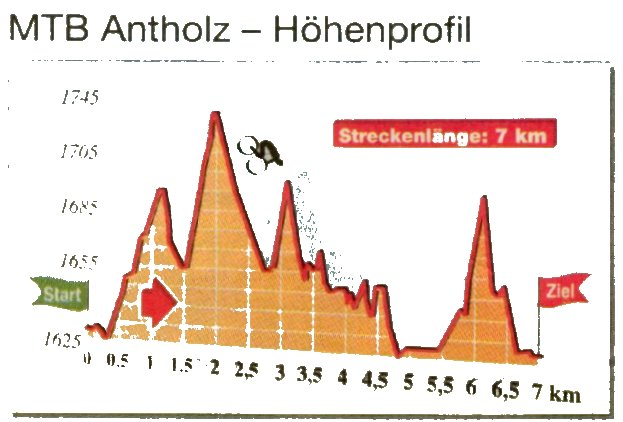
\includegraphics[width=6.5cm]{2te/funktion/bilder/antholz.jpg}
\end{minipage}
\begin{minipage}{7cm}
\bn \item Was wird in der nebenstehenden Graphik zugeordnet? Handelt es sich um eine Funktion?
\item Bestimme die Definitions- und Wertemenge! \en
\end{minipage}

\item Kennst du das Morsealphabet? Handelt es sich dabei um eine Funktion?

\end{enumerate}
\ea




\section{Funktionsgleichung und Funktionswert}

Die Einf\"{u}hrungsbeispiele aus dem vorhergehenden Kapitel stammen zum Teil nicht aus der Mathematik. Sie
sollten aber einen ersten Einblick in diese Materie verschaffen und aufzeigen, dass Funktionen, also
Zuordnungen, uns wirklich \"{u}berall begegnen k\"{o}nnen (wenn wir sie nur erkennen - wollen).

\ba
Versuche selbst eine Funktion aus dem Alltag anzugeben.
\ea

Wir werden uns nun etwas einschr\"{a}nken und uns auf Zahlenbeispiele
konzentrieren. So werden nun f\"{u}r die Definitons- und Wertemenge
meistens Zahlenmengen (z.B. $\mathbb{N, Z, Q, R, R_+} \dots$)
stehen. Wollen wir alle Zahlen zulassen, so wird es sich oft um
Funktionen handeln mit $D= \dots$ und  $W= \dots$, also eine
Zuordnung der Art: $f: \mathbb{R} \mapsto \mathbb{R}$.

Dann ist es aber auch nicht notwendig, jedes Mal diese Mengen eigens anzugeben. So schreiben wir dann z.B.
f\"{u}r die Funktion
\[\begin{array}{rrcl}
  f: & \mathbb{R} & \rightarrow & \mathbb{R} \\
   & x & \mapsto & x^2-1
\end{array}\]
nur mehr die sog. Funktionsgleichung $f(x)=x^2-1$ oder $y=x^2-1$. Dies bedeutet, dass $y$ gleich $f(x)$
(lies: "`f von x"') zu sehen ist. Genauer:

\bd \label{9}
Jede beliebige Funktion
\[\begin{array}{rrcl}
  f: & \mathbb{R} & \rightarrow & \mathbb{R} \\
   & x & \mapsto & y
\end{array}\] besitzt eine {\bf Funktionsgleichung}, n\"{a}mlich
y=f(x). Dabei handelt es sich um eine Gleichung mit zwei
Variablen.
\ed

\bb\label{2.1}
Wie lautet die Funktionsgleichung zur Funktion:
\[\begin{array}{rrcl}
  f: & \mathbb{R} & \rightarrow & \mathbb{R} \\
   & x & \mapsto & -\frac{x}{3}?
\end{array}\]
Wieviele L\"{o}sungen hat diese Gleichung? Gib zwei L\"{o}sungen an.
\eb

\bd
Wenn $f$ eine Funktion ist, so versteht man unter dem {\bf Funktionswert} von $x$, kurz $f(x)$ (lies: "`f von x"'),
jene Zahl, die durch die Funktion $f$ der Zahl $x$ zugeordnet wird.
\ed

\bb
Gegeben ist die Funktion: $f(x)=x^2-2x$. Berechne die
Funktionswert $f(2)$ und $f(-\frac{2}{3})$.
\eb

\ba \label{5}  \label{2.2}
\begin{enumerate}
\item Was ist eine Funktion?
\item Bestimme die Funktionswerte $f(0)$ und $f(\frac{1}{2})$ f\"{u}r
die Funktion $f(x)=4x^2-2x+1$.
\item Bestimme die Funktionsgleichung zur Funktion
\[\begin{array}{rrcl}
  f: & \mathbb{R} & \rightarrow & \mathbb{R} \\
   & x & \mapsto & \frac{7x-3}{2}
\end{array}\] und berechne $\frac{5}{7}$.

\item Gegeben ist die Funktion, die jeder Seitenl\"{a}nge den Umfang
des Quadrates zuordnet. Gib dazu die Funktion samt Definitions-
und Wertemenge und die Funktionsgleichung an. Berechne einige
Funktionswerte, indem du die folgende Tabelle ausf\"{u}llst:
\[\begin{array}{|c|c|c|c|c|c|}
\hline
  x & 1 & 2 & 8 & 10 & -4 \\ \hline
  f(x) &  &  &  &  & \\ \hline
\end{array}\]
\end{enumerate}
\ea



\section{Der Graph der Funktion und die Nullstellen}


\bb {\tiny .}

\begin{minipage}{8cm}
Funktionsgraphen begegnen uns sehr h\"{a}ufig immer und \"{u}berall - beispielsweise in den Medien, in Schulb\"{u}chern
anderer F\"{a}cher (!) und vielerorts mehr.

Nur oft werden die entsprechenden Graphiken nicht mit dem Begriff der Funktion in Verbindung gebracht, oder
auch nur (um etwa den Leser und Betrachter nicht abzuschrecken) nicht erw\"{a}hnt.

Hier ein Beispiel einer typischen Anwendung des Funktionsgraphen zur Veranschaulichung eines komplizierten
Sachverhaltes.

\end{minipage}
\begin{minipage}{6cm}
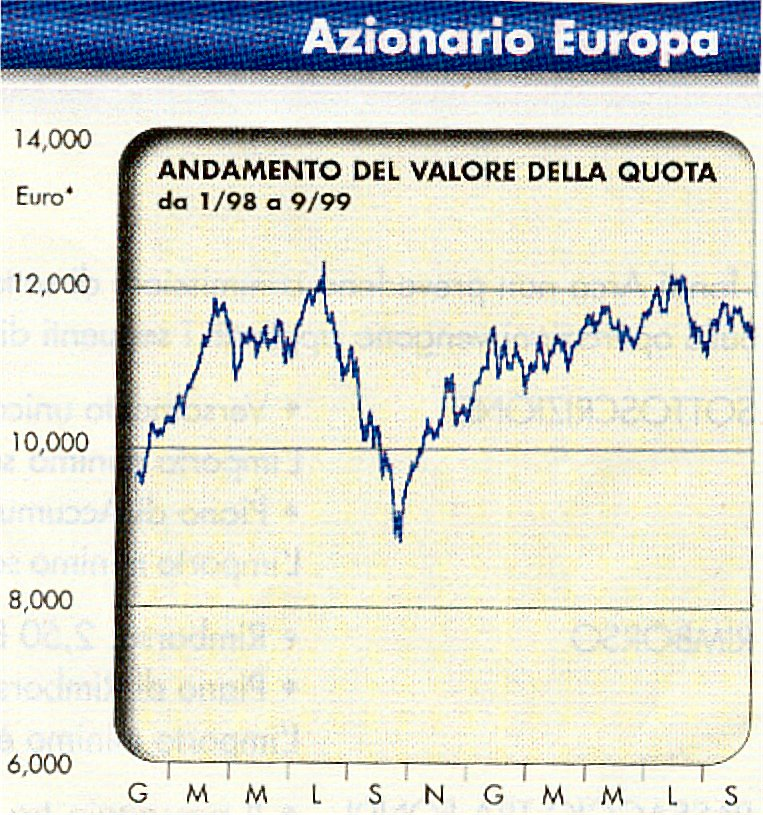
\includegraphics[width=5cm]{2te/funktion/bilder/fkt_aktien.jpg}
\end{minipage}

\eb


Haben wir eine mathematische Funktion, also eine Funktion von $f: \mathbb{R} \rightarrow \mathbb{R}$,
gegeben, so wird jeder (reellen) Zahl $x$ eine Zahl $y$ zugeordnet. Daraus ergeben sich Zahlenpaare $(x;y)$,
die in ein (kartesisches\footnote{nach R.~Descartes, genannt Cartesius, 1596 bis 1650. Die Besonderheit
dieses Koordinatensystems ist, das die Achsen zueinander rechtwinklig sind.}) Koordinatensystem eingezeichnet
werden k\"{o}nnen. So erh\"{a}lt man eine graphische Darstellung einer Funktion - den Graphen der Funktion. Genauer:

\bd
Unter dem {\bf Graph der Funktion} $f$ versteht man die Menge aller Zahlenpaare $(x;f(x))$.
\ed

\begin{Bem}{\bf Praktische Konstruktion des Graphen:}
\begin{enumerate}
\item Man stellt eine Wertetabelle auf, indem man f\"{u}r gen\"{u}gend viele,
geeignet gew\"{a}hlte Zahlen den Funktionswert berechnet. Tip: die Zahl $0$ sollte in der Regel immer gew\"{a}hlt
werden, da die Berechnung des Funktionswerte oft sehr einfach ist. (Was man unter "`gen\"{u}gend viele"' und
"`geeignet gew\"{a}hlte"' Zahlen versteht, h\"{a}ngt von der gegebenen Funktion ab; einige Erfahrung ist sicherlich
daf\"{u}r notwendig.)
\item Man zeichnet diese Zahlenpaare in einem Koordinatensystem
ein und verbindet sie durch eine Kurve (oder Geraden). Dabei
k\"{o}nnen die Einheiten auf der x- und y-Achse beliebig und
verschieden (!) geeignet gew\"{a}hlt werden.
 \end{enumerate}
\end{Bem}

\bb
 Zeichne die Funktionsgraphen der folgenden Funktionen:
\label{6}\label{2.3}\label{2.4}
\begin{enumerate}
\item $f(x)=\frac{1}{2}x$
\item $f(x)=-2x+1$
\item $f(x)=x^2-1$
\end{enumerate}
\eb

\ba Zeichne die Funktionsgraphen der folgenden Funktionen:
\label{8}\label{2.5}
\begin{enumerate}
\item $f(x)=-x$
\item $f(x)=|x|$ (Betragsfunktion, vgl. p. \pageref{7})
\item $f(x)=-x^2+4$
\end{enumerate}


\item Welche Darstellungen geh�ren zu einer Funktion?

%\begin{center}
%\includegraphics[width=7cm]{scanimage200501.jpg}
%\end{center}


\ea

\begin{Bem}
\begin{enumerate}
\item Die eingezeichneten Punkte d\"{u}rfen nur dann verbunden werden,
wenn $D=\mathbb{R}$ ist. Handelt es sich z.B. um eine Zuordnung
zwischen Personen und Eintrittsgeld bei einem Theaterbesuch, so
hat ein Verbinden der Punkte keinen Sinn; warum?
\item Der Funktionsgraph ist sehr sehr n\"{u}tzlich. Oft, vor allem im
Alltag, z.B. in Zeitschriten, in Lehrb\"{u}chern usw. wird auf die
Angabe der Funktion verzichtet und nur der Funktionsgraph
dargestellt. Weiters dient er:
\begin{enumerate}
\item zur Veranschaulichung der Funktion
\item zur graphischen Bestimmung von Funktionswerten (x gegeben, y
gesucht)
\item zur graphischen Bestimmung der Werte x, die durch die
Funktion einem bestimmten $y$ zugeordnet werden ($x$ gesucht, $y$
gegeben).
\item zur graphischen Bestimmung der Schnittpunkte des
Funktionsgraphen mit der x-Achse; dies f\"{u}hrt zur folgenden
Definition:
\end{enumerate}
\end{enumerate}
\end{Bem}

\bd
Gegeben ist eine Funktion $f$. Ein $x \in D$ bezeichnet man als
{\bf Nullstelle}, falls $f(x)=0$ gilt.
\ed

Man sucht also die Werte aus der Definitionsmenge die den
Funktionswert $0$ ergeben. Dies sind dann eben genau die
Schnittpunkte des Funktionsgraphen mit der x-Achse.

\bb
\begin{enumerate}
\item  Ermittle graphisch $f(-2)$ und $f(4)$ von Bsp. \ref{6} Nr. 2.
Bestimme weiters die Nullstellen. Kontrolliere deine Ergebnisse
rechnerisch.
\item Ermittle graphisch alle $x$, f\"{u}r die $y=9$ bzw. $y=2$ ist
aus Bsp. \ref{6} Nr. 3. Gibt es Nullstellen? Kontrolliere wieder
deine Ergebnisse rechnerisch.
\end{enumerate}
\eb




\ba
Diese Aufgabe bezieht sich auf die 3 Funktionen aus Aufgabe
\ref{8} Nr.1, 2 und 3:
\begin{enumerate}
\item Zeichne die 3 Graphen indem du dir gen\"{u}gend Funktionswerte berechnest.
\item Bestimme jeweils $f(1)$ graphisch und kontrolliere rechnerisch.
\item Bestimme (ungef\"{a}hr) alle $x$, so dass $f(x)=8$ gilt.
\"{U}berpr\"{u}fe dein Ergebnis rechnerisch.
\item Bestimme die Nullstellen zeichnerisch und rechnerisch.
\end{enumerate}
\ea

\begin{Bem}{\bf Zusammenhang: Graph und Funktionsgleichung}
Wie in Definition \ref{9} auf Seite \pageref{9} erw\"{a}hnt, handelt
es sich bei der Funktionsgleichung um eine Gleichung mit zwei
Variablen. Eine Gleichung dieser Art hat unendlich viele L\"{o}sungen,
denn man kann sich einfach f\"{u}r eine Variable eine Zahl w\"{a}hlen und
die andere berechnen.

Andererseits kann eine Funktionsgleichung dazu verwendet werden um
Zahlenpaare zu berechnen, die, eingezeichnet in ein
Koordinatensystem, den Funktionsgraphen ergeben.

Zusammenhang: der Funktionsgraph besteht aus den L\"{o}sungen der
Funktionsgleichung oder umgekehrt:

jede L\"{o}sung der Funktionsgleichung, also jedes Zahlenpaar, das die
Funktionsgleichung erf\"{u}llt, liegt auf dem Graphen der Funktion.
\end{Bem}

\bn \item 
Gegeben ist die Funktion $f(x)=-x+5$. \label{2.6} \"{U}berpr\"{u}fe
 zeichnerisch und  rechnerisch
ob die Punkte $(0;0)$, $(-\frac{7}{2};8,5)$ und $(4;2)$ auf dem Funktionsgraphen liegen und somit L\"{o}sungen
der Funktionsgleichung sind.
\item 
 Liegen die Punkte $(3;9)$ und $(-2;-4)$ auf dem Graphen der Funktion $f(x)=x^2$?  Begr\"{u}nde zeichnerisch und  rechnerisch! Berechne auch die  Nullstellen dieser Funktion! 
\en



\section{Umkehrfunktionen}

\subsection{Allgemeine Definition und Beispiele}
 \bd  Die Funktion $f: D \rightarrow W$ mit $D, W \subseteq \mathbb{R}$ hei{\ss}t {\it bijektiv} oder {\it
umkehrbar}, wenn gilt: \bn \item F\"{u}r alle $x_1, x_2 \in D$ mit $x_1 \neq x_2$ gilt: $f(x_1)\neq f(x_2)$;
\item f\"{u}r jedes $y \in W$ gibt es ein $x \in D$ mit $f(x)=y$.\en  \ed  

\ba \bn \item Gib eine Beispiel f\"{u}r eine umkehrbare (bijektive) Funktion an. \item Finde zwei Beispiele von
Funktionen, welche nicht umkehrbar sind, wobei beim ersten Beispiel die erste Bedingung und beim zweiten
Beispiel die 2. Bedingung nicht erf\"{u}llt ist. Visualisiere den Sachverhalt mit Hilfe von einem Pfeildiagramm
(2 Mengen und die Zuordnung zeichnen). \en \ea  

\bd  Ist $f$ umkehrbar, dann ist durch $$f^{-1}(y)=x
:\Leftrightarrow f(x)=y$$ eine Funktion $f^{-1}:D \rightarrow W$ definiert, welche als {\bf Umkehrfunktion}
oder auch {\it inverse Funktion} von $f$ bezeichnet wird. \ed  

\begin{Bem}
Per Definition gilt: $f^{-1}(f(x))=x \qquad \mbox{f\"{u}r alle} \quad x \in D \qquad \mbox{und} \qquad
f(f^{-1}(x))=x \qquad \mbox{f\"{u}r alle} \quad x \in D$
\end{Bem}

Es gibt auch unendlich viele Funktionen, die keine Umkehrfunktion besitzen. Schr\"{a}nkt man aber die
Definitionsmenge ein, so kann man eine Umkehrfunktion angeben.

\bb Die Funktion $y=x^4$ ist auf $D=\mathbb{R}$ nicht umkehrbar. Nimmt man aber $D=\mathbb{R}^+$ so ist die
Funktion streng monoton und deshalb umkehrbar.\eb



\bs  \label{dfdf} Die Graphen von $f$ und $f^{-1}$ im kartesischen Koordinatensystem sind {\it symmetrisch}
bez\"{u}glich der ersten Winkelhalbierenden $y=x$. \es 

Damit bekommen wir auch eine Anleitung zum Auffinden einer Umkehrfunktion:

Ist $f$ umkehrbar, so gewinnt man die Funktionsgleichung von $f^{-1}$ durch (formales) Vertauschen der
Variablen in $y=f(x)$ und Aufl\"{o}sen nach $y$: $$y=f(x) \qquad \Rightarrow \qquad x=f(y)   \qquad  \Rightarrow \qquad f^{-1}(x)=y$$

\ba \bn \item Finde die Umkehrfunktion zu $f(x)=-\frac12x+3$ und zeichne beide Funktionsgrafen in das gleiche
Koordinatensystem ein. \"{U}berpr\"{u}fe anschlie{\ss}end Satz \ref{dfdf} (Seite \pageref{dfdf}).
\item Gegeben sei die Funktion $f(x)=\sqrt{x}$ und der Definitionsbereich $\{9,16,25,36\}$.     Bestimme den
Wertebereich der Funktion. Bestimme ihre Umkehrfunktion. Bestimme Definitionsbereich und Wertebereich der Umkehrfunktion.
\en
\ea

\bme 
{\bf �ber die Umkehrung einer Funktion}
\bn \item
Jede {\it streng monoton wachsende} oder {\it fallende} Funktion ist {\it umkehrbar}
\item Bei der Umkehrung einer Funktion werden Definitions- und Wertemenge miteinander vertauscht.
\item Die Umkehrfunktion $g$ einer Funktion $y=f(x)$ findet man  (oft aber nicht immer) indem man  \bn \item  $y$ und $x$ vertaucht \item und nach $y$ wieder die Gleichung aufl�st.\en 
\item Zeichnerisch erh�lt man das Schaubild der Umkehrfunktion durch {\it Spiegelung} des Funktionsgraphen an der 1. Winkelhalbierenden (Gerade: $y=x$)
 
\en 
\eme 



\subsection*{\"{U}bungen zur Schularbeit}
\ba
\begin{enumerate}
\item $g$ ist die Funktion, die jeder rationalen Zahl ihr Quadrat
zuordnet. \bn \item Dann gilt: \[\begin{array}{ccccc}
  g(2)=\dots & g(0)=\dots & g(4)=\dots & g(\frac{1}{2})=\dots & g(0,4)=\dots \\
  g(3)=\dots & g(1)=\dots & g(-4)=\dots & g(-\frac{1}{3})=\dots & g(-0,5)=\dots
\end{array}\]
\item Zeichne mit diesen berechneten Werten den Funktionsgraph.
\item Wie lautet die Funktionsgleichung?
\item Wie m\"{u}ssen Definitionsmenge und/oder Wertemenge ver\"{a}ndert werden, damit eine Umkehrfunktion existiert?
Wie lautet ihre Funktionsgleichung? \en

\item Erg\"{a}nze:

{\it Eine Funktion $f$ ist eine $\dots$. Sie ordnet jeder Zahl $x$
ihrer $\dots$ wieder eine Zahl zu, den. sog. $\dots$ von $x$
(Bezeichnung: $\dots$).

Zwischen $f$ und $f(x)$ besteht der folgende Unterschied: $f$
bezeichnet die $\dots$, dagegen ist $f(x)$ eine $\dots$.}

\item Die Funktion $g$ ist definiert durch $g(x)=x^2+2x$.
\begin{enumerate}
\item Die Funktion $g$ hat die Definitionsmenge $D=\dots$.
\item Berechne $g(3)$, $g(\frac{5}{2})$, $g(-3)$ und $g(1)$!
\item Gib an: $g(z)=\dots$, $g(u)=\dots$.
\item Welche Zahlen haben den Funktionswert $8$?
\item Gibt es Nullstellen?

\end{enumerate}

\item Wir betrachten die Funktion
\[\begin{array}{rrcl}
  h:  & u & \mapsto & \frac{u}{u^2-4}
\end{array}\]
Welchen Definitionsbereich hat $h$? Berechne $h(1)$, $h(10)$,
$h(-\frac{3}{2})$ und $h(2)$.
\item
\begin{enumerate}
\item Zeichne den Graphen von $g(x)=0,6\cdot x+1$.
\item Um was f\"{u}r eine Kurve handelt es sich offensichtlich?
\item Wie viele Punkte h\"{a}tten also f\"{u}r das Zeichnen des Graphen
gen\"{u}gt? \item Berechne die Nullstellen! \item Bestimme die Funktionsgleichung der Umkehrfunktion.
\end{enumerate}
\item
\begin{enumerate}
\item Erg\"{a}nze:

{\it Unter einer L\"{o}sung der Gleichung \[y=2-\frac{1}{5}x^2\]
versteht man ein $\dots$, das beim Einsetzen in die Gleichung
diese $\dots$.}

\item Versuche so eine L\"{o}sung anzugeben.

\item Liegen die Punkte $P=(-4,5;-2)$ und $Q=(-1,5;1,6)$ auf dem
Graphen dieser Funktion? \end{enumerate}
\item Kann die Kurve aus der Abbildung  der Graph einer Funktion
sein? Warum nicht?

\input{2te/funktion/bilder/fkt1.pic}

\item Kann eine horizontale Gerade der Graph einer Funktion sein?

Kann eine vertikale Gerade der Graph einer Funktion sein?
\end{enumerate}

\ea



\chapter{Lineare Funktionen}
Nachdem wir den Begriff der Funktion allgemein untersucht haben,
beginnen wir in diesem Abschnitt mit der n\"{a}heren Betrachtung
einzelner Funktionstypen. Die einfachste dieser Funktionenklassen
sind die {\it linearen Funktionen}.










\section{Definition und Eigenschaften}
\subsection{Begriff und Beispiele}
\bd 
Eine Funktion $f$ nennt man {\bf linear}, wenn ihre
Funktionsgleichung auf die Form $$y=k\cdot x + d \qquad \qquad (k, d \in
\mathbb{R})$$ gebracht werden kann.
 \ed  



\ba  Entscheide, welche der folgenden Funktionsgleichungen
linear sind und bestimme gegebenenfalls $k$ und $d$.
\[\begin{array}{lll}
  a.)\quad 3x-4y =7 &   b.)\quad x=y-3x+6 &   c.)\quad \frac{1}{y}=\frac{x}{y}+4 \\
  d.)\quad y=-\frac{2x}{3}+\frac{4}{7} &   e.)\quad y=2x^2-3&   f.)\quad
  y=6-x
\end{array}\]
\ea 

\subsection{Eigenschaften}
Lineare Funktionen sind f\"{u}r uns nicht neu. Sie sind uns schon im
vorhergehenden Abschnitt begegnet und wir haben in Beispielen und
Hausaufgaben sogar schon sechs Graphen von linearen Funktionen
gezeichnet.
\begin{longtable}{p{5cm}p{5cm}p{5cm}}
  Graph 1: $y=-\frac{x}{3}$ &
  Graph 2: $y=\frac{7x-3}{2}$ & 
   Graph 3: $y=\frac{1}{2}x$ \\
      (Bsp. \ref{2.1} Seite \pageref{2.1}) &
   (Auf. \ref{2.2} Seite \pageref{2.2}) & 
  (Bsp. \ref{2.3} Seite \pageref{2.3})\\
   
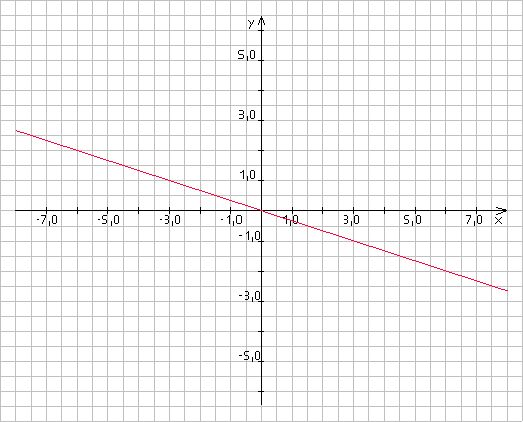
\includegraphics[width=4.5cm]{2te/linearefunktion/bilder/lf1.jpg} & 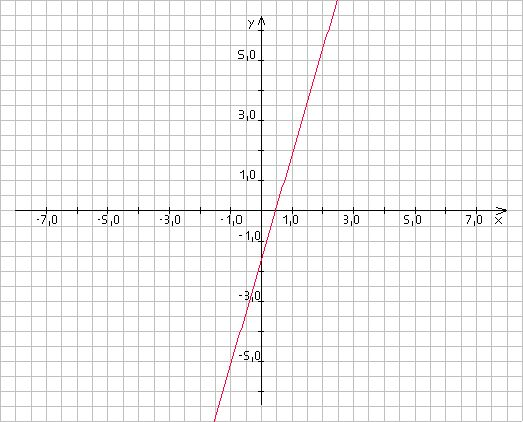
\includegraphics[width=4.5cm]{2te/linearefunktion/bilder/lf2.jpg}&
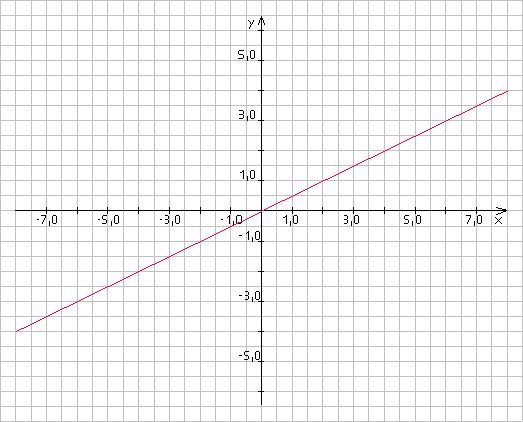
\includegraphics[width=4.5cm]{2te/linearefunktion/bilder/lf3.jpg} \\

Graph 4: $y=-2x+1$ 
  & Graph 5: $y=-x$  &
  Graph 6: $y=-x+5$  \\
 (Bsp. \ref{2.4} Seite \pageref{2.4})&
  (Auf. \ref{2.5} Seite \pageref{2.5}) &
   (Bsp. \ref{2.6} Seite \pageref{2.6})  \\
   
   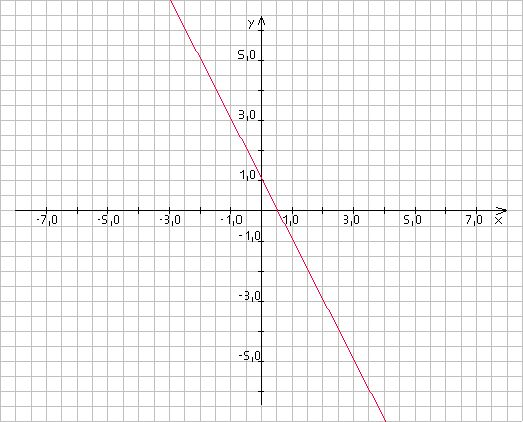
\includegraphics[width=4.5cm]{2te/linearefunktion/bilder/lf4.jpg}&
  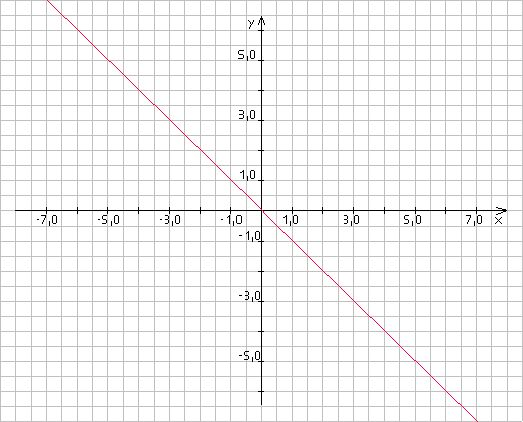
\includegraphics[width=4.5cm]{2te/linearefunktion/bilder/lf5.jpg} & 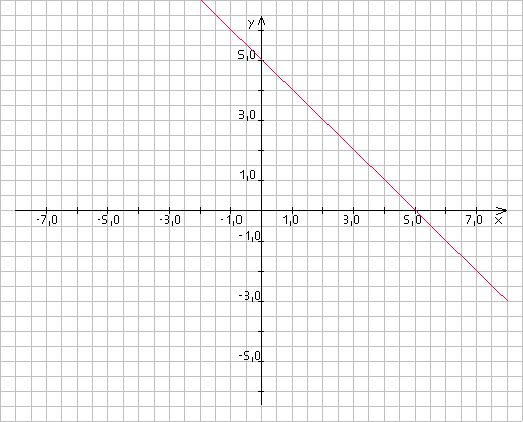
\includegraphics[width=4.5cm]{2te/linearefunktion/bilder/lf6.jpg}\\
\end{longtable}



\ba {\bf Computerraum}

Wir haben nun die Aufgabe festzustellen, wie die Graphen der
linearen Funktionen von $k$ und $d$ abh\"{a}ngen. 

�ffne dazu die Datei {\tt ../materialien/linearefunktion.gxt} und arbeite den Arbeitsauftrag sorgf�ltig durch:

\begin{enumerate}

\item Stelle zun�chst f�r die Konstanten (falls nicht schon
eingestellt) folgende Werte ein: $k=0,d=0$. �ndere nun mit der
Maus den Wert f�r $d$. Beobachte, was sich genau ver�ndert und
halte deine Beobachtungen fest!

\item Setze nun $k=1$ und ver�ndere den Wert f�r
$d$. Halte wie oben deine Beobachtungen fest! 

\item $d$ wird "`$y-$Achsenabschnitt"' genannt. Warum glaubst du, ist das so?

\item Setze $d$ auf den Wert $0$. Ver�ndere nun den Wert $k$ und
halte alle deine Beobachtungen fest! Gehe besonders auf die nachfolgenden Fragen ein

\begin{enumerate}
\item Was passiert f�r ein positives bzw. negatives $k$?
\item Gibt es eine M�glichkeit anhand der Steigung der Geraden zu erkennen, wie gro� $k$ gew�hlt wurde? 
\item $k$ wird "`Steigung"' genannt. Wie k�nnte Steigung, auch im Alltagsleben, definiert sein (z.B. im Sta�enverkehr)?

\end{enumerate}

\item W�hle nun selbst einige Werte f�r $k$ und $d$. Halte deine Beobachtungen fest.

\item �berpr�fe, ob �berall \textbf{ausf�hrlich in ganzen S�tzen}
geantwortet wurde. Versuche schlie�lich die Antworten auf obige
Fragen auf eine Seite (maximal zwei) zu bringen und in einer
ansehnlichen Form darzustellen. Drucke die Seite(n) aus!

\item \textbf{F�r all jene, die fr�her fertig werden:} �berlege dir eine Methode, mit der man erstens ohne Berechnung einer Wertetabelle den Graphen einer linearen Funktion finden kann, und zweitens anhand eines Graphen die Funktionsvorschrift bestimmen kann.

\end{enumerate}




\ea

Die Ergebnisse dieser Beobachtung formulieren wir als
Merksatz:

\bme \label{3satz}
\begin{enumerate}
\item Der Graph einer linearen Funktion ist immer $\dots$.
\item Die Steigung dieser Geraden h\"{a}ngt von der Variablen $k$ ab:
\begin{enumerate}
\item Ist k positiv ($k>0$), so $\dots$
\item Ist k negativ ($k<0$), so $\dots$
\item Ist $k =0$, so $\dots$
\end{enumerate}
\item  Je gr\"{o}{\ss}er $|k|$ ist, umso $\dots$ \hspace{2cm} verl\"{a}uft die Gerade.
\item Der Graph schneidet die y-Achse im Punkt $\dots$
\item Wenn $d=0$ ist, die lineare Funktion also die Form $y= \dots$ hat,
so verl\"{a}uft der Graph immer durch den $\dots$.

\end{enumerate}
\eme

 \bd  
\bi \item Gegeben ist eine lineare Funktion $f(x)=kx+d$. Die Variable $k$ nennt man {\bf Steigung}, die Variable $d$
ist der {\bf y-Achsenabschnitt} des Graphen.
\item 
Den Schnittpunkt der x-Achse mit der y-Achse in einem
Koordinatenkreuz nennt man {\bf Ursprung} oder {\bf Nullpunkt}
$(0/0)$.\ei
 \ed  




\ba 

\bn \item  Welcher Graf geh�rt zu welcher Gleichung?

	\begin{minipage}{6cm}
	\bi \item $f_1(x)=3x-4$;\item $f_2(x)=-3x-4$; \item $f_3(x)=\frac13x-4$; \item $f_4(x)=-\frac13x$; \item $f_5(x)=-4$\ei
	\end{minipage} 
	\begin{minipage}{8cm}
	\begin{center}
		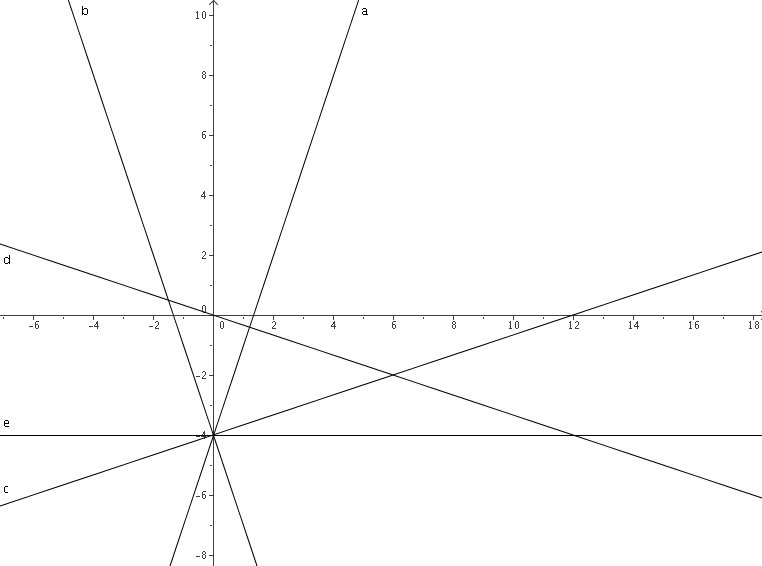
\includegraphics[width=8cm]{2te/linearefunktion/bilder/200502.jpg}
		\end{center}
	\end{minipage}


	\item "`9 Bildchen"'

	\begin{minipage}{6cm}
	$k>0$, $k=0$, $k<0$ sind 3 verschiedene F�lle. Das gleiche gilt f�r $d$. Somit gibt es $9$ verschiedene M�glichkeiten. Zeichne alle Beispiele und beschrifte aussagend.
	\end{minipage} 
	\begin{minipage}{8cm}
	\begin{center}
		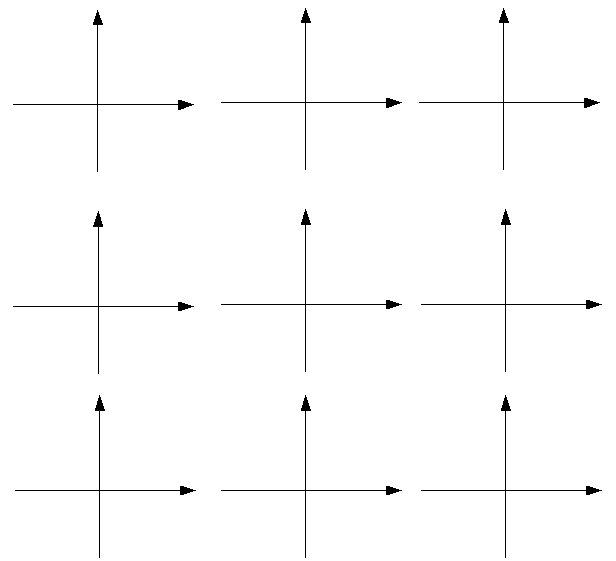
\includegraphics[width=8cm]{2te/linearefunktion/bilder/200501.jpg}
		\end{center}
	\end{minipage}


\item \bn \item Es sei $k$ eine fix gew�hlte Variable. Was haben alle m�glichen Funktionsgrafen der Funktionen $y=kx+d$ gemeinsam? Zeichne ein Schaubild.
\item Es sei $d$ eine fix gew�hlte Variable. Was haben alle m�glichen Funktionsgrafen der Funktionen $y=kx+d$ gemeinsam? Zeichne ein Schaubild.
\en \en
\ea 




\subsection{Der Graph der linearen Funktion}
\subsubsection{Praktische Zeichnung von linearen Funktionsgraphen}

Da der Graph einer linearen Funktion immer eine Gerade ist, so
ben\"{o}tigt man zum genauen Zeichnen des Graphen nur {\it 2 Punkte},
denn eine Gerade ist durch 2 Punkte ja eindeutig festgelegt.

Dabei brauchen wir effektiv nur mehr einen Punkt berechnen, da
einer schon aus der Funktionsgleichung herausgelesen werden kann,
n\"{a}mlich: ($\dots$). (Warum?)

\bb  
Zeichne den Graphen von $y=\frac{x}{2}-4$
\eb  


\subsubsection{Besondere Graphen}

 \bd  \label{defdsdf}
\bi \item Eine Funktion $f$ hei�t {\bf konstant}, falls $f(x)=c$ mit $c \in \mathbb{R}$ ist.

\item Die {\bf Betragsfunktion} $$f(x)=|x|$$ ordnet jedem Zahl ihren Abstand vom Nullpunkt auf dem Zahlenstrahl zu.

\item Die {\bf Signumfunktion} ist die sog. Vorzeichenfunktion, sie ordnet allen positiven Zahl die Zahl $+1$, den negativen die Zahl $-1$ und der Zahl $0$ die $0$ zu.

\item Die {\bf Treppenfunktion} $f(x)=[x]$ entsteht dadurch, dass jeder Zahl ihr "`Gr��tes Ganzes"' zugeordnet wird. \ei
 \ed  

\ba Zeichne jeweils einen bzw. den Funktionsgraf zu Definition \ref{defdsdf}.\ea


\subsection{Nullstellen und lineare Gleichungen}

Wir haben schon in der Einf\"{u}hrung von Derive gesehen, dass jede
beliebige Gleichung zeichnerisch mit Hilfe des Funktionsgraphen
gel\"{o}st werden kann: die L\"{o}sung(en) der Gleichung ergibt bzw.
ergeben sich als Nullstelle(n) des Funktionsgraphen.

Der Vorteil dieser f\"{u}r die Mathematik wichtigen Erkenntnis liegt
darin, dass damit eine Methode bekannt ist, um komplizierte
Gleichungen zumindest n\"{a}herungsweise zu l\"{o}sen. Denn es gibt
Gleichungen, die mit algebraischen Umformungsmethoden nicht exakt
gel\"{o}st werden k\"{o}nnen. So k\"{o}nnen beispielsweise bei Gleichungen
h\"{o}heren Grades (z.B. $3x^5-3x^3+4x=9$) die ersten Schwierigkeiten
auftreten.

In diesem Kapitel hat die graphische Methode noch nicht eine so gro{\ss}e Bedeutung, da ja die Berechnung von
Nullstellen einer linearen Funktion auf eine \hspace{3cm} Gleichung f\"{u}hrt, die ja mit den Methoden der ersten
Klasse einfach gel\"{o}st werden kann.


\ba 
Ermittle die Nullstellen von $y=\frac14 x-2$ zeichnerisch und
\ea 

Die letzte Aufgabe und das letzte Beispiel f\"{u}hren auf die Frage,
ob eine lineare Funktion immer eine Nullstelle hat und wenn ja, ob
es immer genau eine ist:

\bs  \label{sdfsfgg}
Eine lineare Funktion $y=kx+d$ besitzt
\begin{enumerate}
\item genau eine Nullstelle, falls $\dots$
\item unendlich viele Nullstellen, falls $\dots$
\item keine Nullstelle, falls $\dots$
\end{enumerate}
\es  

Diesen Satz \ref{sdfsfgg} kann man sehr sch\"{o}n graphisch interpretieren:

\begin{center}
\begin{pspicture}(15,4)
\mygrid
\end{pspicture}
\end{center}



\subsection{Berechnung der Funktionsgleichung}
In der Praxis treffen wir selten auf Funktionsgleichungen. Dagegen
sind sehr oft zwei Gr\"{o}{\ss}en gegeben, die voneinander abh\"{a}ngen
($\rightarrow$ Funktionen!). Dabei sind konkret meistens Werte
gegeben, also mathematisch gesehen Zahlenpaare $(x,y)$, mit denen
man dann evtl. ein Schaubild oder Diagramm ($\rightarrow$
Funktionsgraph) zeichnet, oder mit denen man andere Werte
ausrechnen soll ($\rightarrow$ Funktionswerte/Nullstellen).

Wenn es um konkrete Beispiele aus der Praxis geht, dann k�nnen verschiedene Fragestellungen sehr einfach mit Hilfe einer vorhandenen Funktionsgleichung beantwortet werden.\bn \item Es kann zu jedem beliebigen $x$ das entsprechende $f(x)$ sehr einfach durch
Einsetzen des Wertes in die Funktionsgleichung berechnet werden. \item es kann zu jedem gegebenen $y$ durch
das Aufl\"{o}sen der (linearen!) Gleichung das entsprechende $x$ berechnet werden.\en

Diesen Sachverhalt soll das folgende (in Wahrheit etwas vereinfachte Beispiel - in der Praxis ist eine
"`Kostenfunktion"' sehr wahrscheinlich nicht linear) Beispiel noch einmal unterstreichen:

\bb Ein Betrieb produziert Schildm\"{u}tzen  und hat dabei (fixe und variable) Kosten, die von den produzierten
St\"{u}ckzahlen abh\"{a}ngen. Im letzten Monat hat die Produktion von $5.000$ St\"{u}ck Kosten in H\"{o}he von $30.000$ \euro
\, ergeben. Im Vormonat ergaben sich Kosten in H\"{o}he von $36.000$ \euro bei einer Produktion von $6.000$
St\"{u}ck. \bn \item Wie hoch sid die Kosten bei einer Produktion von $5.000$ M\"{u}tzen? \item Wie viele M\"{u}tzen
k\"{o}nnen mit einem Budget von $50.000$ \euro \, produziert werden? \en\eb


An dieser Stelle soll gezeigt werden, wie man aus gegebenen Werten die Funtionsgleichung berechnet. Im
n\"{a}chsten Abschnitt treffen wir auf zahlreiche Anwendungsgebiete von linearen Funktionen.

Setzen wir die zwei gegebenen Punkte $(x_1/y_1)$ und $(x_2/y_2)$  in die Funktionsgleichung $y=kx+d$ ein, so
ergeben sich $2$ (lineare) Gleichungen mit $2$ Unbekannten, n\"{a}mlich $k$ und $d$. Die Aufgabe lautet nun aus
den gegebenen $2$ Gleichungen die $2$ Unbekannten auszurechnen. 

\bb \label{bboben} W�hle selbst zwei beliebige Punkte $P_1$ und $P_2$. Berechne die lineare Funktion, deren Graph durch diese zwei Punkte verl�uft. Kontrolliere dein Ergebnis anhand einer Zeichnung.\eb


%Dies f\"{u}hrt uns auf das folgende Kapitel: \input{lin_gs.tex}

Ist die Funktionsgleichung $y=kx+d$ gesucht, dann hei{\ss}t dies, dass
die Steigung $k$ und der y-Achsenabschnitt $d$ zu berechnen sind.
Eine erste Hilfe bietet dabei der folgende Satz:

\bs  \label{ssoben}
Sind zwei Punkte $(x_1/y_1)$ und $(x_2/y_2)$ gegeben, so kann die
Steigung $k$ daraus wie folgt berechnet werden:
\[k=\frac{y_2-y_1}{x_2-x_1}\]
\es  
\begin{proof}
1. Geometrisch ({\bf Steigungsdreieck})\hspace{5cm} 2. Rechnerisch 

\begin{center}
\begin{pspicture}(15,5)
\mygrid
\end{pspicture}
\end{center}

\end{proof}


\bb Berechne Beispiel \ref{bboben} mit Hilfe von Satz \ref{ssoben}.\eb





\subsection{Lineare Gleichungssysteme und lineare Funktionen}\label{linfkl_lings}


\subsubsection{Die Funktionsgleichung $y=kx+d$ ist gesucht}
Jedem leuchtet die geometrische Aussage "`Durch zwei Punkte verl\"{a}uft genau eine Gerade"' ein. Diese Aussage
kann demnach dazu benutzt werden, um die Funktionsgleichung zu berechnen, falls zwei Punkte des
Funktionsgraphen bekannt sind:

\bb Welche lineare Funktion verl\"{a}uft durch $P=(-3/2)$ und $Q=(\frac{1}{2}/-\frac{1}{2})$? \eb

Achtung: Falls wir die Funktionsgleichung wie \"{u}blich mit $y=kx+d$ bezeichnen, so sind jetzt nicht $x$ und
$y$, sondern $k$ und $d$ gesucht!

Ist die Steigung $k$ oder der y-Achsenabschnitt $d$ und ein weitere Punkt bekannt, so erh\"{a}lt man durch das
Einsetzen in die Funktionsgleichung eine lineare Gleichung mit einer Unbekannten, die sehr einfach gel\"{o}st
werden kann.

Damit haben wir alle n\"{o}tigen Kenntnisse gesammelt und k\"{o}nnen nun anhand der verschiedenen Aufgaben dieses
neue Wissen ein\"{u}ben:
\ba 
\begin{enumerate}
\item Welche lineare Funktion verl\"{a}uft durch die Punkte $(3/-4)$ und
$(-2/3)$?
\item Berechne die Funktionsgleichung der Funktion mit der
Steigung $\frac{2}{3}$, die die y-Achse bei $-\frac{2}{5}$ schneidet.
\item Welcher Funktionsgraph geht durch den Punkt
$(23,2/\frac{25}{7})$ und hat die Steigung $0,2$?
\item Liegen die folgenden drei Punkte auf einer Geraden?
A=$(1/4)$, B=$(2/1)$ und C=$(3/-1)$ - \"{U}berpr\"{u}fe rechnerisch und zeichnerisch. 

\item Von einer Geraden sind zwei Punkte $P_1=(1/1)$ und
$P_2=(7/-5)$ bekannt.
\begin{enumerate}
\item Zeichne die Gerade
\item Wie lautet die Funktionsgleichung? Versuche diese Frage zuerst
graphisch anhand von a.) n\"{a}herungsweise zu l\"{o}sen und \"{u}berpr\"{u}fe dein Ergebnis rechnerisch.
\item Berechne die Nullstelle - kontrolliere das Ergebnis mit a.).
\end{enumerate}

\item 
{\bf Computerraum} "`St�ckweise definierte Funktionsgrafen"'
Zeichne mit Hilfe einer passenden Software eine "`nette"' Figur. Z.B. Namen schreiben.
\end{enumerate}
\ea 

\subsubsection{Der Schnittpunkt zweier lin. Funktionen  ist gesucht}
Diese Art der Anwendung haben wir schon kennengelernt und muss hier eigentlich nicht mehr wiederholt werden.

\bb {\tiny .}

a) $\quad$ 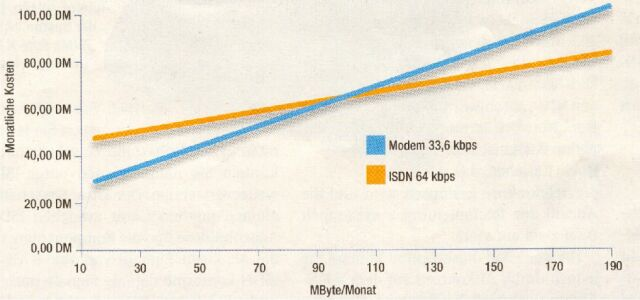
\includegraphics[width=5.5cm]{2te/linearefunktion/bilder/modem.jpg}   \qquad \qquad   b) $\quad$  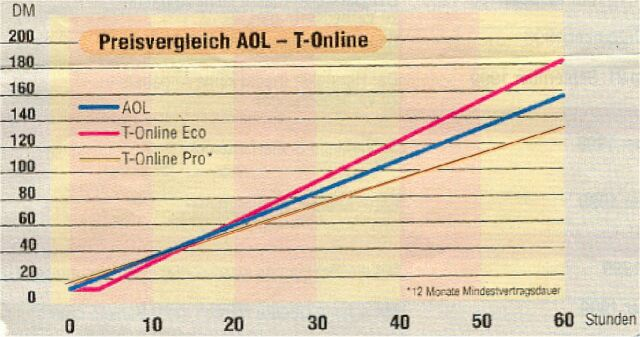
\includegraphics[width=5.5cm]{2te/linearefunktion/bilder/aol.jpg}
 \eb

 \ba Gegeben sind die Funktionen $f(x)=\frac{2}{3}x+3$ und $g(x)=x-\frac{1}{3}$. Bestimme den Schnittpunkt der
 Funktionsgraphen! \ea

\ba
�bung Computerraum:

�ffne die Seite \begin{verbatim}
http://www.cybernautenshop.de/virtuelle_schule/lehrinhalte_index2.html
\end{verbatim}
und gehe zu den abgebildeten Kapiteln. Gute Arbeit!

\begin{center}
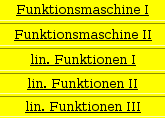
\includegraphics[width=3cm]{2te/linearefunktion/bilder/funktionen.png}
\end{center}

\ea 

\section{Anwendungen der linearen Funktion}
Anhand der folgenden Beispiele soll gezeigt werden wie verbreitet lineare Funktionen sind. Praktisch findet man in
allen Berufen Beispiele f\"{u}r diese Funktionsart.

\bb  
\begin{enumerate}
\item {\bf Proportionalit\"{a}ten}

$3$ kg einer Ware kosten $4,5$ Euro.
\begin{enumerate}
\item Wieviel kosten $7$ kg der Ware?
\item Wie lautet die Funktionsgleichung?
\item Zeichne den Graphen f\"{u}r $x \in\{1, \dots, 10\}$.
\item Kontrolliere dein Ergebnis aus a.) zeichnerisch!
\item Wieviel $kg$ bekomme ich f\"{u}r $10$ Euro. Beantworte die Frage zeichnerisch und rechnerisch!
\end{enumerate}
\item {\bf Prozentrechnung}

Die Mehrwertsteuer betr\"{a}gt zur Zeit $20\%$ vom Warenwert. Sie h\"{a}ngt also direkt vom Warenwert ab.
\begin{enumerate}
\item Wieviel Euro betr\"{a}gt die MWSt., wenn der Warenpreis $20$, $30$, $50$, $70$, $85$ bzw. $100$ Euro betr\"{a}gt?
\item Wie lautet die Funktionsgleichung?
\item Zeichne den Graphen bis $x=100$.
\end{enumerate}

\item {\bf Fixe und variable Kosten}

 Ein Gaswerk berechnet f\"{u}r $1m^3$ Gas einen Preis von $0,2$ Euro bei einer monatlichen Grundgeb\"{u}hr von $3$ Euro.
\begin{enumerate}
\item Bilde die Funktionsgleichung, die den Zusammenhang zwischen Gasmenge und Rechnungspreis angibt.
\item Zeichne das Bild der Funktion bis zu einem Verbrauch von $10m^3$.
\item Zu welcher Zahlenmenge geh\"{o}ren die y-Werte?
\item Wieviel bezahlt man bei einem Verbrauch von $16m^3$ Gas? L\"{o}se rechnerisch und zeichnerisch!
\item Wieviel hat man verbraucht, wenn auf der Betrag von $59$ Euro zu bezahlen ist? L\"{o}se rechnerisch und zeichnerisch!
\end{enumerate}

\item {\bf Gegeben: Zahlenpaare}
Das Gehalt eines Vertreters setzt sich aus einem Grundgehalt und einem Prozentsatz an Provision zusammen. Aufgrund
seiner letzten zwei Gehaltsstreifen wei{\ss} er, dass er bei einem Umsatz von $40.000$ Euro ein Gehalt von $4.000$ Euro und
bei einem Umsatz von $20.000$ Euro ein Gehalt von $2.800$ Euro erh\"{a}lt. Kannst du aus diesen Informationen sein
Grundgehalt und seinen Provisionssatz ermitteln?

\item {\bf Bestimmung des Schnittpunktes}
In einem Beh\"{a}lter befinden sich $40$ Liter Wasser. In jeder Sekunde flie{\ss}en $0,5$ Liter hinzu. In einem zweiten
Beh\"{a}lter befinden sich $25$ Liter Wasser. Der Zufluss betr\"{a}gt $1,2$ Liter pro Sekunde. Nach wievielen Sekunden befindet
sich in beiden Beh\"{a}ltern die gleiche Wassermenge und wieviel? L\"{o}se diese Aufgabe zeichnerisch und rechnerisch.
\end{enumerate}
\eb  

\section*{�bungen - Vorbereitung auf die Schularbeit}
\ba 
\begin{enumerate}
\item $1$ Dollar kostet $1,5$ Euro.
\begin{enumerate}
\item Formuliere den Zusammenhang zwischen den W\"{a}hrungen als lineare Funktion.
\item Zeichne den Graphen dieser Funktion.
\item Wie viel Dollar bekommt man f\"{u}r $6$ Euro. Beantworte diese Frage zeichnerisch und rechnerisch.
\item Wie viel Euro bekommt man f\"{u}r $30$ Dollar? Beantworte diese Frage ebenfalls zeichnerisch und rechnerisch.
\end{enumerate}
\item Die Zinsen h\"{a}ngen direkt vom Kapital ab. Angenommen der Zinssatz betr\"{a}gt $5\%$, so bekommt man f\"{u}r ein Kapital von
$100$ Euro $5$ Euro an Zinsen.
\begin{enumerate}
\item Formuliere den Zusammenhang zwischen Kapital und Zinsen als lineare Funktion.
\item Zeichne den Graphen dieser Funktion.
\item Wie viel betragen die Zinsen bei einem Kapital von $1.600$ Euro? Beantworte diese Frage zeichnerisch und rechnerisch.
\item Bei welchem Kapital bekommt man $50$ Euro an Zinsen? Beantworte diese Frage ebenfalls zeichnerisch und rechnerisch.
\end{enumerate}

\item Die fixen Kosten eines Betriebes betragen monatlich $12.000$ Euro. Der Kostenpreis pro St\"{u}ck des produzierten
Artikels betr\"{a}gt hingegen $6$ Euro.
\begin{enumerate}
\item Wie lautet die Funktionsgleichung, die den Zusammenhang zwischen St\"{u}ckpreis und Gesamtkosten darstellt?
\item Zeichne das Bild dieser Funktion.
\item Wieviel St\"{u}ck k\"{o}nnen produziert werden, damit der gesamte Kostenpreis nicht mehr als $20.000$ Euro betr\"{a}gt.
Beantworte diese Frage zeichnerisch und rechnerisch.
\end{enumerate}
\item Das neue Tarifsystem der SAD f\"{u}r \"{U}berlandfahrten setzt sich aus einer einmaligen Tagesgeb\"{u}hr und ein variabler Betrag
pro gefahrener Kilometer zusammen. Wie hoch ist diese Tagesgeb\"{u}hr und wieviel bezahlt man pro Kilometer, wenn
jemand von St. Martin nach Meran (18km) $1,4$ \euro \, bezahlt und am n\"{a}chsten Tag von Meran nach Lana (9km)
f\"{u}r $0,85$ \euro \, weiterf\"{a}hrt? Wie lautet schlie{\ss}lich die Funktionsgleichung, die den gefahrenen
Tageskilometern den Preis zuordnet?



\item

%\begin{minipage}{6cm}
Bestimme die Gleichungssysteme, welche zu den entsprechenden Grafen passen.
%\end{minipage}
%\begin{minipage}{10cm}
\begin{center}
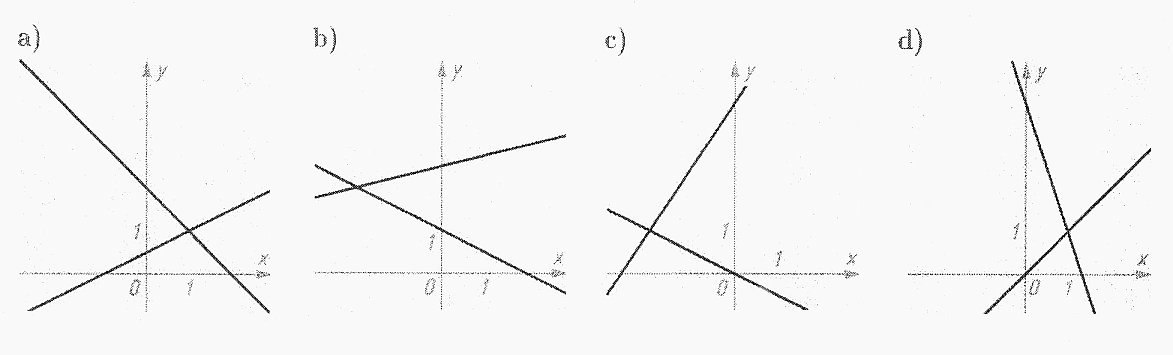
\includegraphics[width=10cm]{2te/linearefunktion/bilder/scanimage200502.jpg}
\end{center}


%\end{minipage}



\item Ein �ltank enth�lt  $1000$ l Heiz�l. Pro Tag werden $35$ l verbraucht.
\bn \item Stelle die Restmenge $R(t)$, die nach $t$ Tagen �brig ist, als Funktion von $t$ dar.
\item Wie viel �l ist nach $14$ Tagen noch im Tank?
\item Wann ist der Tank leer? \en

\item In einer Stadt waren im Jahr 1990 ca. $7200$ PKW zugelassen, im Jahr 2000 ca. $11700$. Man kann annehmen, dass die Anzahl der PKW linear w�chst.
\bn \item Wie viele PKW werden pro Jahr neu zugelassen?
\item Stelle die Anzahl der PKW als Funktion der Zeit dar (1990 = Jahr 0).
\item Wie viele PKW sind im Jahr 2010 zu erwarten?
\item Wann wird es voraussichtlich $18.000$ PKW geben?\en




\item

%\begin{minipage}{6cm}
Drei verschiedene Geraden k�nnen unterschiedlich viele Schnittpukte miteinander haben. Erstelle f�r
alle vier F�lle ein Gleichungssystem.
%\end{minipage}
%\begin{minipage}{10cm}
\begin{center}
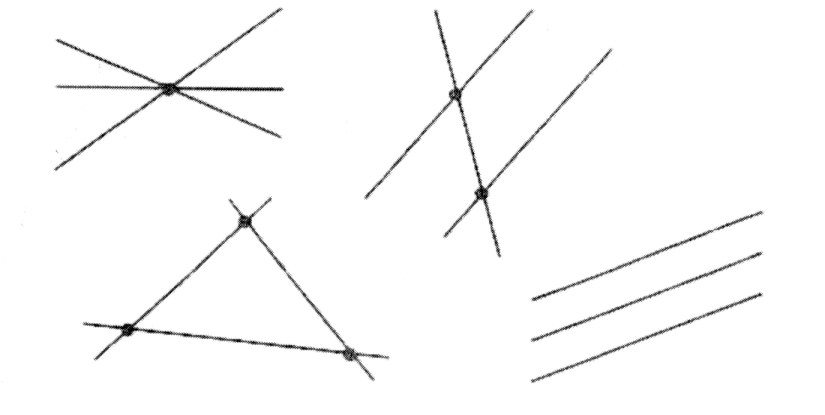
\includegraphics[width=8cm]{2te/linearefunktion/bilder/scanimage200503.jpg}
\end{center}


%\end{minipage}

\item Eine Taxifahrt kostet $2,50$  Euro Grundgeb�hr und $0,96$ Euro pro gefahrenem Kilometer.
\bn \item Stelle den Fahrpreis $F(x)$ als Funktion der Strecke $x$ dar.
\item Wie viel kostet eine $6$ km lange Fahrt?
\item Wie weit kann man mit $10$  Euro  fahren? \en



\item Die Nachbarsh�ndin Senta jagt oft die Katze Minka. 

%\begin{minipage}{6cm}
\bn \item Erfinde sinnvolle Geschichten zu den folgenden Graphen.
\item Stelle zu den drei Abbildungen passende Geradengleichungen auf.
\item Versuche jeweils de Geschwindigkeit von der H�ndin und der Katze zu bestimmen. Wo findest du diese in der jeweiligen Geradengleichung wieder?
\en
%\end{minipage}
%\begin{minipage}{10cm}
\begin{center}

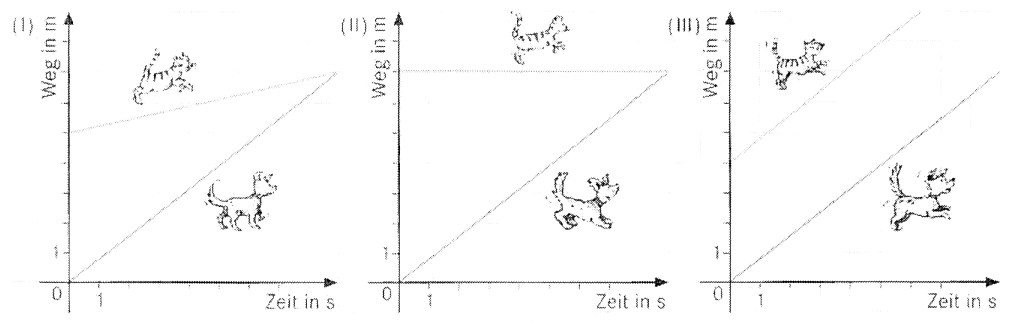
\includegraphics[width=10cm]{2te/linearefunktion/bilder/scanimage200504.jpg}
\end{center}

%\end{minipage}





\item Internetkosten

\bi \item Der Internet-Provider  www.freewebster.com bietet als Superkn�ller die Surfstunde zu $0,50$ Euro an. Allerdings muss man eine monatliche Grundgeb�hr von $5$ Euro bezahlen. 

\item Die Firma www.billigsurfen.com wirbt damit, dass ihr Angebot, eine Surfstunde von $1,50$ Euro pro Stunde und ohne Grundgeb�hr, das g�nstigste Angebot derzeit auf dem Markt sei.
\ei

L�se grafisch und rechnerisch.



\item Ein Elektrizit\"{a}tswerk bietet zwei Tarife an:\\
Tarif1: Grundgeb\"{u}hr $9$ Euro und $0,12$ Euro pro Kilowattstunde.\\ Tarif2: Grundgeb\"{u}hr $12$ Euro und $0,08$ Euro pro
Kilowattstunde.
\begin{enumerate}
\item Bilde beide Funktionsgleichungen!
\item Bei welchen Stromverbrauch ergibt sich der gleiche Rechnungsbetrag. Wann ist also Tarif1 und wann Tarif2
g\"{u}nstiger. Beantworte diese Frage zeichnerisch und rechnerisch!
\end{enumerate}


\item R�tsel:




	\begin{center}
	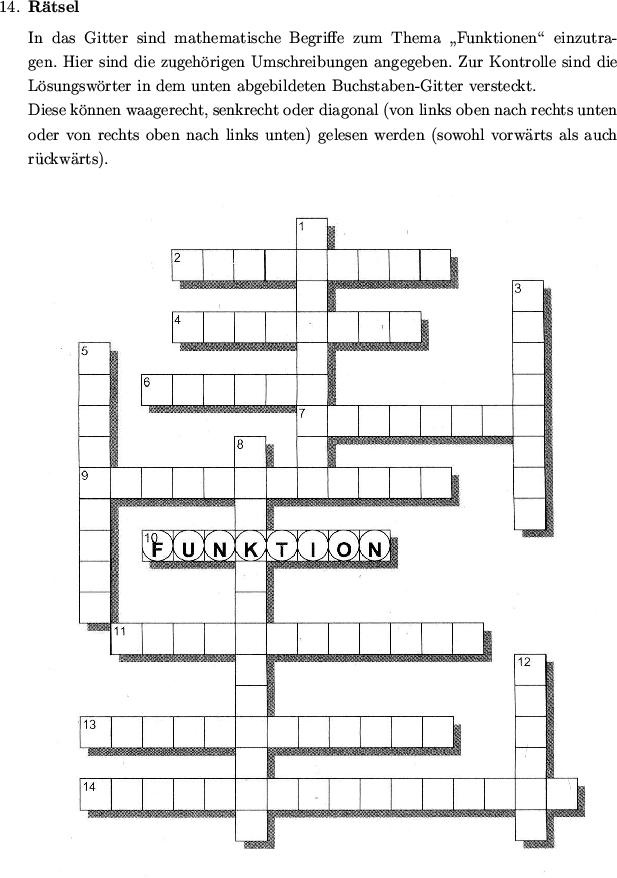
\includegraphics[width=9cm,angle=90]{2te/linearefunktion/bilder/scanimage200506.jpg}
	\end{center}
	
	\begin{center}
	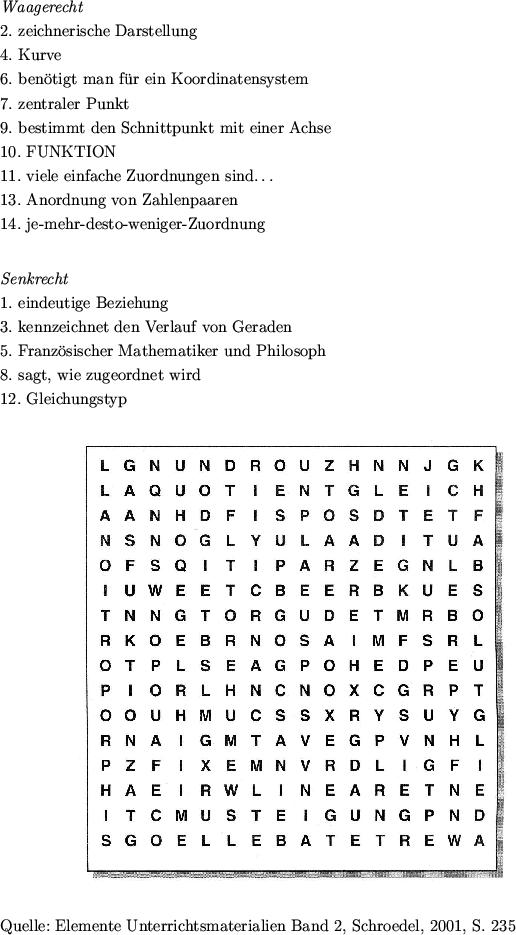
\includegraphics[width=8cm,angle=90]{2te/linearefunktion/bilder/scanimage200505.jpg}
	\end{center}
\end{enumerate}
\ea 


\subsection*{Noch mehr �bungen (mit L�sugen)}

\ba
.../skripten/2te/linearefunktion/uebungenlinearefunktion.tex
\ea


 \chapter{Die reellen Zahlen}

\begin{minipage}{9cm}
\bd  Die {\bf Quadratwurzel} einer positiven Zahl $a$ ist diejenige {\it positive} Zahl, deren Quadrat gleich $a$ ist. Bezeichnung: $\sqrt{a}$: $$\left(\sqrt{a}\right)^2=a$$\ed  
\end{minipage}
\begin{minipage}{4cm}

\includegraphics[width=4cm]{2te/reellezahlen/bilder/logo2.jpg}
\end{minipage}


\ba \bn \item  {\bf Wiederholung} \bn \item Wof�r stehen die Symbole $\mathbb{N, Z,}$ und $\mathbb{Q}$? \item Was sind periodische Dezimalzahlen? \item Wie k�nnen endliche, wie periodische Dezimalzahlen als Bruch dargestellt werden?\en 


\item Vereinfache ohne Taschenrechner:
$$\begin{array}{lll}
a.) \quad \sqrt{64}= \qquad & \qquad \qquad & b.) \quad \sqrt{\frac49}= \qquad \\
c.) \quad \sqrt{\frac{32}{18}}= \qquad & \qquad \qquad & d.) \quad \sqrt{6+\frac14}= \qquad \\
e.) \quad \sqrt{2,25}= \qquad & \qquad \qquad & f.) \quad \sqrt{0,\overline{1}}= \qquad \\
\end{array}$$
\item Warum muss $a$ positiv sein?
\item Wenn jeder positiven Zahl ihre Wurzel zugeordnet wird, dann handelt es sich ja wieder um eine Funktion. Nenne Definitions- und Wertemenge dieser Funktion und zeichne ihren Grafen.
\en \ea


\section{Die irrationalen Zahlen}
\subsection{Die Zahl $\sqrt{2}$}

\begin{minipage}{7cm}\bb Gegeben ist ein Quadrat mit der Seitenl�nge $1$. Wie lang ist eine Diagonale?\eb
\end{minipage}
\begin{minipage}{5cm} \end{minipage}

\vspace{1.5cm}

\ba {\bf �berlegungen zu $\sqrt{2}$} Was verbirgt sich nun hinter $\sqrt{2}$? Wie sieht die Zahl aus? Wie kann man sie hinschreiben? Kann man sie hinschreiben???

\bn \item  Versuche $\sqrt{2}$ m�glichst gut mit einem Bruch auszudr�cken. Wer schafft es auf m�glichst viele Stellen genau?\footnote{Mein Bruch, den es zu "`schlagen"' gilt: $\frac{11}{8}$.}

\item Der Taschenrechner: Vielleicht hilft uns der Taschenrechner? Berechne die $\sqrt{2}$ mit Hilfe des Taschenrechners, notiere das Ergebnis und mache die Probe. Was stellst du fest?

\item Der Zahlenstrahl: Wo befindet sich die Zahl auf dem Zahlenstrahl? Kannst du die Stelle geometrisch exakt einzeichnen? 

\vspace{2cm}


\vspace{1cm}
\en
\ea


\bs  $\sqrt{2}$ kann nicht als Bruch dargestellt werden, also handelt es sich nicht um eine rationale Zahl, kurz: $$\sqrt{2} \in ...$$
\es 

\begin{minipage}{10cm}
\begin{proof}Beispiel eines {\it indirekten Beweises}. Man nimmt eine Aussage als wahr an, folgert daraus eine Widerspruch und hat damit gezeigt dass die angenommene Aussage falsch war.

Hier hei�t die Aussage: Es gibt einen Bruch $\frac{a}{b}$ mit $a, b \mathbb{N}$ geben, so dass gilt:  $$\frac{a}{b}=\sqrt{2}$$
Wir wissen: jede nat�rliche Zahl kann eindeutig in ein Produkt von Primfaktoren zerlegt werden. Vergleicht man die Anzahl der Primzahlen von $2a^2$ und $b^2$, so ist sie nicht gleich! Also, kann die Gleichung $\frac{a^2}{b^2}=2$ nicht wahr sein und damit war die Aussage falsch. Also: $\sqrt{2}$ ist keine rationale Zahl. 
\end{proof}
\end{minipage}
\begin{minipage}{5cm}
	\begin{center}
	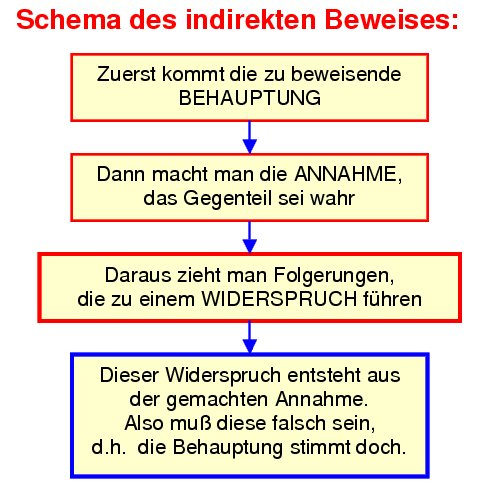
\includegraphics[width=5cm,bb=0 0 501 489]{2te/reellezahlen/bilder/indirekterbeweis.jpg}
% indirekterbeweis.jpg: 83dpi, width=15.33cm, height=14.96cm, bb=0 0 501 489
	\end{center}
\end{minipage}



\begin{minipage}{10cm}
\begin{Folg}
Man kann $\sqrt{2}$ nicht als endliche Dezimalzahl hinschreiben, lediglich n�herungsweise:
\bn \item mit Hilfe eines Taschenrechners (... Stellen): ...
\item Gedicht von Aigner: daneben findest du ein Gedicht von Prof. Alexander Aigner. Damit kann die Quadratwurzel von $2$ auf $42$ Stellen genau angegeben werden:

Jedes Wort hat eine Buchstabenzahl, die die Ziffer an der entsprechenden Dezimalstele angibt. Ist die Buchstabenanzahl gr��er als $9$, musst du solange $10$ abziehen, bis eine Zahl kleiner als $10$ herauskommt. (Sonderzeichen nicht mitz�hlen). Vor dem Komma steht eine $1$, da "`O"' ein Buchstabe ist. Nach dem Komma folge eine $4$, da "`kann"' aus $4$ Buchstaben besteht.
 
\item Computer (Millionen von Stellen) (z.B. mit Mupad).

\en\end{Folg}
\end{minipage}
\begin{minipage}{5.2cm}
\begin{flushright}
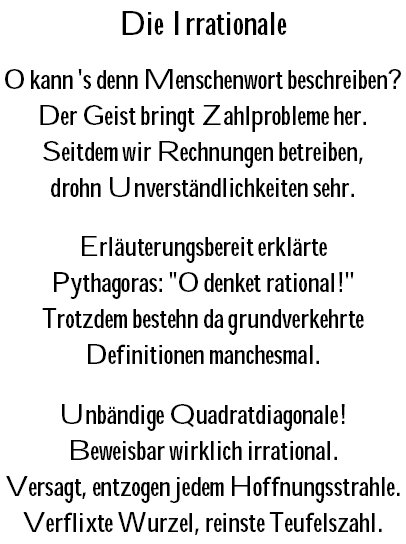
\includegraphics[width=5.2cm]{2te/reellezahlen/bilder/aigner.jpg}
\end{flushright}
\end{minipage}

\paragraph*{Fazit:}

\bs  Alle nat�rlichen Zahlen, die keine Quadratzahlen (z.B. $1, 4, 9, 16, 25, ...$) sind, haben keine rationale Quadratwurzel.\es 
 


\bd  \bi \item Eine {\bf irrationale Zahl} ist eine unendliche, nicht periodische Dezimalzahl.
\item Eine {\bf reelle Zahl} ist eine (endliche oder unendliche, periodische oder nicht periodische Dezimalzahl. 
 \item Die Menge alle reellen Zahlen wird mit $\mathbb{R}$ bezeichnet.\ei\ed 


\ba
 \bn \item Berechne (ohne Taschenrechner):

\bt{llllllll}
 a) & $\sqrt{49} $ & b) & $\sqrt{\frac{1}{16}} $ &
  c) & $\sqrt{\frac{50}{72}} $ & d) & $\sqrt{7+\sqrt{81}} $ \et
\item Stelle fest, ob folgende Zahlen rational oder irrational
sind und kreuze an!

\bt{l|l|c|c}
 & Zahl & rational & irrational \\ \hline
 a) & $5,121212\dots$ & $\Box$ & $\Box$ \\
 b) & $5,121221222122221\dots$ & $\Box$ & $\Box$   \\
 c) & $5,121$ & $\Box$ & $\Box$  \\
 d) & $0,343344333444\dots$ & $\Box$ & $\Box$   \\
 e) & $0,343344333444$ & $\Box$ & $\Box$  \\ \et


\item Welche der folgenden Aussagen ist richtig? Kreuze an!

\bt{lll}

a)& Jede nat\"{u}rliche Zahl ist eine reelle Zahl.& $\Box$ \\

b)& Jede nat\"{u}rliche Zahl ist eine irrationale Zahl. & $\Box$ \\

c)& Jede rationale Zahl ist eine irrationale Zahl. & $\Box$ \\

d)& Jede ganze Zahl ist eine rationale Zahl. & $\Box$ \\

e)& Jede ganze Zahl ist eine reelle Zahl. & $\Box$ \\

f)& Jede rationale Zahl ist eine reelle Zahl. & $\Box$ \\

g)& Jede nat\"{u}rliche Zahl ist eine rationale Zahl. & $\Box$ \\

h)& Jede reelle Zahl ist eine irrationale Zahl. & $\Box$ \\

i)& Jede reelle Zahl ist eine rationale Zahl. & $\Box$  \et 

 \item Zeichne rechts von obiger Definition ein aussagekr�ftiges Mengendiagramm f�r $\mathbb{N, Z, Q, R}$ und zeichne jeweils ein Zahlenbeispiel an.  \item Beweise, dass  $\sqrt{8}$ irrational ist. \item Warum funktioniert der Beweis f�r $\sqrt{4}$ nicht?
 \item {\it In jedem Intervall $[a, b]$ mit $a, b \in \mathbb{R}$ gibt es unendlich viele irrationale Zahlen!}

Was h�ltst du von dieser Aussage?

\item Die irrationalen Zahlen historisch betrachtet: seit wann etwa sind irrationale Zahlen anerkannt? Wer leistete dabei Beachtliches?  Wie gingen die antiken Griechen (Pythagoras und andere) mit diesem Ph�nomen um? Recherchiere dazu im Internet.

\item Gehe auf die Seite \href{http://www.mathe-online.at/tests/zahlen/zahlenmengen.html}{http://www.mathe-online.at/tests/zahlen/zahlenmengen.html} und f�hre den Multiple Choice Test mit Mehrfachantworten zum Thema Zahlenmengen durch.
\en 
\ea


\section{Darstellung einer irrationalen Zahl}

\subsection{N�herungsverfahren}
\paragraph{Kostruieren und Ablesen}:

\begin{minipage}{7cm}
Wie kann man $\sqrt{n}$ mit $n \in \mathbb{N}$ konstruieren? Die Antwort gibt die nebenstehende Grafik und der Satz des Pythagoras. Der Haken dieser Konstruktion: es muss die $\sqrt{n-1}$ schon konstruiert sein. Man spricht dabei von {\it rekursiv}.
\end{minipage}
\begin{minipage}{8cm}
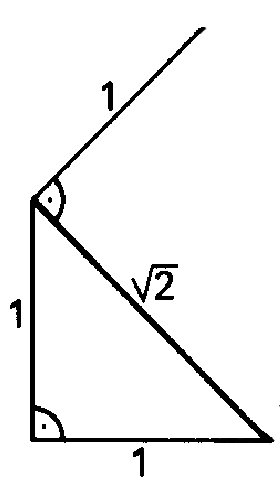
\includegraphics[width=2.5cm]{2te/reellezahlen/bilder/konstruktionwurzel.jpg}
\end{minipage}


\begin{minipage}{7cm}
(Siehe */materialien/RechtecksflaecheQuadratWurzelfunktion.gxt). Sucht man zu einem gegebenen Rechteck mit der Fl�che $F$ ein fl�chengleiches Quadrat, so kann diese Aufgabe konstruktiv mit Hilfe des H�hensatzes gel�st werden. Dabei ergibt sich f�r die Seitenl�nge $s$ des Quadrates: $$s=\sqrt{A}$$
Welche Ortskurve erh�lt man nun, wenn die Rechtecksbreite gleich $1$ (eins) gew�hlt wird?
\end{minipage}
\begin{minipage}{8cm}
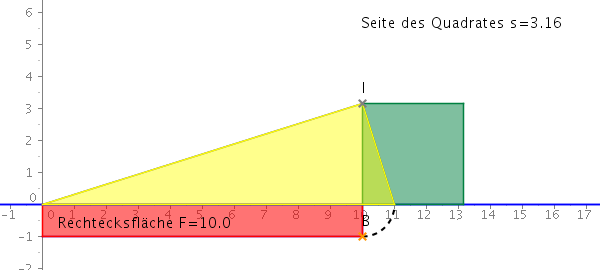
\includegraphics[width=8cm]{2te/reellezahlen/bilder/rechtecksflaeche.png}
\end{minipage}

\paragraph{Intervallschachtelung}
\ba {\bf Computerraum} Schau dir die Pr�sentation "`Intervallschachtelung"' konzentriert an.\ea

Das {\bf Intervallschachtelungsprinzip} bildet in der Numerischen Mathematik die Grundlage f�r einige L�sungsverfahren.

Das Prinzip ist einfach: Man f�ngt mit einem Intervall an und "`nimmt"' sich aus diesem Intervall ein Intervall, das komplett in dem vorherigen Intervall drin liegt, und "`nimmt"' sich dort wieder ein Intervall raus und so weiter. Die Intervalle sind ineinander verschachtelt. Durch die unendliche Hintereinanderausf�hrung zieht sich das Intervall immer mehr zusammen bis es nur noch ein einziger Punkt ist.  Eine Strategie k�nnte sein, das Intervall fortlaufend zu {\it halbieren}, dann spricht man vom sog. {\bf Intervallhalbierungsverfahren}.

Der Vorteil dieses Verfahrens ist, dass es recht einfach, der Nachteil, dass es sehr aufwendig ist!
	\begin{center}
	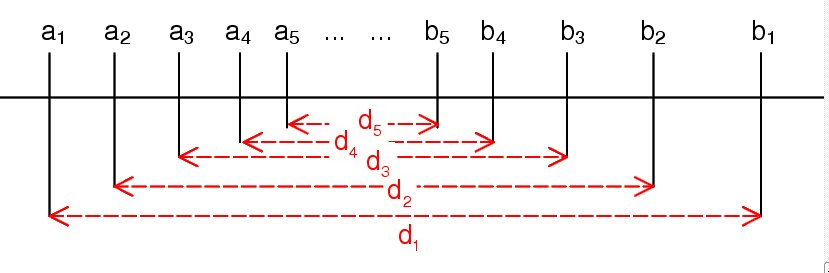
\includegraphics[width=14cm,bb=0 0 829 273]{2te/reellezahlen/bilder/intervallschachtelung1.jpg}
% intervallschachtelung1.jpg: 83dpi, width=25.37cm, height=8.35cm, bb=0 0 829 273
	\end{center}

\bd  Die (unendlich vielen) Intervalle rationaler Zahlen bilden eine {\bf Intervallschachtelung}, wenn gilt:
\bn \item Jedes Intervall ist im vorangehenden enthalten. \item Die Intervalll�ngen nehmen ab und werden beliebig klein. \en \ed

\begin{Folg}
Die Intervallschachtelung bestimmt auf der Zahlengeraden genau einen Punkt.
\end{Folg}

\bb F�hre das Intervallhalbierungsverfahren f�r $\sqrt{20}$ durch. Gesucht ist eine auf $5$ Dezimalstellen genaue L�sung.\eb

\ba Bestimme eine Intervallschachtelung f�r $\frac19=0,\overline{1}$.\ea



\paragraph{Das Heron-Verfahren}
Mit diesem Verfahren kann jeder Ausdruck $\sqrt{n}$ (mit $n \in \mathbb{N}$)  auf beliebig viele Dezimalstellen genau angegeben werden.

Schon um $500$ vor Christus wussten die Griechen, wie man Wurzeln berechnet. Heron von Alexandria hat dies im 1. Jahrhundert nach Christus niedergeschrieben und Isaac Newton (1643-1727) hat dieses Verfahren verallgemeinert.
Die Idee ist genauso genial wie einfach.


\bs  Nach Wahl eines geeigneten Startwertes $x_0$ liefert die wiederholte Berechnung
(Iteration\footnote{(lat.): wiederholen}) nach der Vorschrift

$$x_{n+1}=\frac12\left(x_n+\frac{a}{x_n}\right)\qquad \qquad (a \geq 0; \quad n \in \mathbb{N})$$
eine Folge von immer genaueren N�herungswerten f�r $\sqrt{a}$.\es 


\begin{minipage}{8cm}
\begin{proof}Die n�herungsweise Berechnung von $\sqrt{a}$ f�hrt auf das gleiche Problem, wie die
Bestimmung der Seitenl�nge eines Quadrates mit gegebenen Fl�cheninhalt $A$ - dabei sei $A=a$. Um
die Seitenl�nge eines Quadrates mit dem Fl�cheninhalt $A$ zu berechnen, betrachtete Heron eine
Folge von Rechtecken, die alle den Fl�cheninhalt $A$ haben und sich dem gesuchten Quadrat
annh�hern. 
\end{proof}
\end{minipage}
\begin{minipage}{7cm}
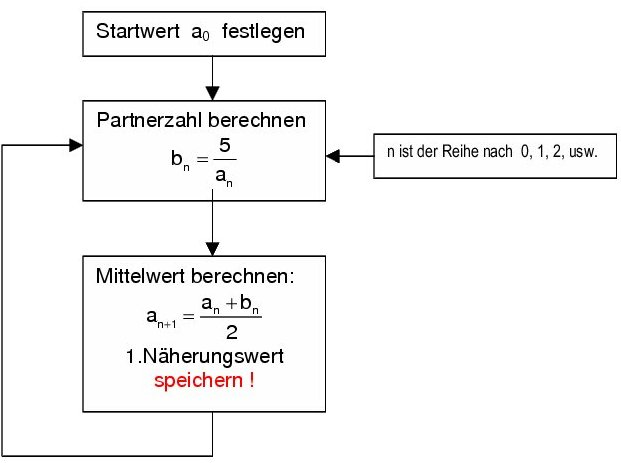
\includegraphics[width=7cm]{2te/reellezahlen/bilder/heron.jpg}
\end{minipage}

\bn
\item Es wird eine beliebige Seitenl�nge $x_0$ des Rechtecks gew�hlt.
\item F�r die  andere Seitenl�nge folgt aus $x_0\cdot y_0=A$: $y_0=\frac{A}{x_0}$.
\item Um ein Rechteck zu erhalten, welches dem Quadrat angen�hert ist, bildet man aus den beiden
Seitenl�ngen das {\bf arithmetische Mittel}: $$x_{neu}=\frac12\left(x+y\right)$$
\item F�r $y_2$ folgt dann: $y_2=\frac{A}{x_2}$
\item Diese Schritte 3 und 4 werden nun beliebig oft wiederholt. Die Folge der dabei errechneten
Rechtecksl�ngen n�hert sich immer mehr der gesuchten Quadratsseitenl�nge.
\item So ergibt sich $$x_{n+1}=\frac12\left(x_n+y_n\right)=\frac12\left(x_n+\frac{A}{x_n}\right)$$\en


\bb Berechne mit dem Heron-Verfahren  einen auf $7$ Stellen genauen N�herungswert f�r $\sqrt{2}$:
%
\begin{center}
\begin{tabular}{|c|p{5cm}|p{5cm}|}
  \hline
  % after \\: \hline or \cline{col1-col2} \cline{col3-col4} ...
  $n$ & $x_n$ & $x_{n+1}$ \\
  \hline
  1 &  &  \\
  2 &  &  \\
  3 &  &  \\
  4 &  &  \\
  $\dots$ &  &  \\
     \hline
\end{tabular}
\end{center}

Da sich schon bei $n=4$ die Werte von $x_n$ und $x_{n+1}$ nicht mehr �ndern, ist die gesuchte
Genauigkeit erreicht. \eb



\ba Berechne mit dem Heron-Verfahren einen auf $7$ Stellen genauen N�herungswert f�r $\sqrt{14}$.
\ea


\ba {\bf Computerraum}

\bn \item Tabellenkalkulation

Erstelle ein Tabellenblatt, das es erlaubt f�r $\sqrt{a}$ jedes beliebige $a$ und einen beliebigen
Startwert einzugeben und sofort (mit Hilfe von Formeln) eine ausgef�llte Tabelle (wie oben) mit
N�herungswerten anzugeben. Weiters soll die Genauigkeit angegeben werden. Bei welcher Stellenanzahl
st��t ein Tabellelkalkulation an seine Grenzen?

\item Derive

Derive hat f�r iterative Berechnungen eine vorgegebene Funktion enthalten. - Hier die Syntax:

\begin{center}{\tt Iterates(Iterationsausdruck, Iterationsvariable, Startwert, Anzahl der
Iterationen)}\end{center}

Das Ergebnis ist eine Folge von Br�chen, welche durch "`Approximieren\footnote{Ann�herung}"' als
Dezimalzahlen dargestellt werden.

(Achtung: sei vorsichtig mit der Anzahl der Iterationen - eine hohe Zahl zwingt auch moderne
Rechner in die Knie...)

 
 \bn \item F�hre jetzt einige Berechnungen durch $\sqrt{2}, \sqrt{14}$

 \item Berechne $\sqrt{216}$ mit Mupad auf $15$ Stellen nach dem Komma genau. Variiere dabei die
 Startwerte: $2; 12,6; 14,7; 21,6; 216$.

 Welchen Einfluss hat der Startwert auf Anzahl der notwendigen Iterationen? Wie sollte man den
 Startwert w�hlen?

 \item �berpr�fe mit Mupad die $42.$ Stelle von $\sqrt{2}$ (vgl. mit dem Gedicht von Prof. Aigner:
 "`Die Irrationale"'.)
\en  \en

\ea

\ba Taschenrechner sind pr�zise und machen nie Fehler. So m�chte man meinen. \bn \item  Dann versuche mal 25-mal die Quadratwurzel aus 10 zu ziehen und anschlie�end 25-mal das Ergebnis zu quadrieren, es m�sste gelten:
$(\sqrt{\sqrt{\sqrt{...\sqrt{10}}}})^2)^2)^2)...)^2=10$. Was stellst du fest?
\item Versuche nun ein CAS zu benutzen, was stellst du fest?
\item Wie schauts mit einer Tabellenkalkulation aus?
\en 
Das Problem ist, dass die Stellenanzeige eines jeden elektronischen Ger�tes begrenzt ist, die Zahlen aber oft unendliche Dezimalzahlen sind. In der Praxis merkt man davon meistens nicht. Auf den Seiten 129 bis 132 sind im Buch "`Mathematik f�r Sonntagmorgen"' einige interessante Episoden aufgelistet, wo diese Rundung doch zu Problemen f�hrte: Raketen, Wetter, Wirtschaft, ... - in unserer Bibliothek.
\ea



\ba F�r Profis - h�here Wurzeln 
\bn \item Bestimme $\sqrt[3]{16}$ auf $100$ Stellen genau.
Schreibe die letzten $10$ Stellen auf. Benutze dabei die Iterationsformel
$$x_{n+1}=\frac13\left(2x_n+\frac{a}{x_n^2}\right)$$ von Heron zur n�herungsweisen Berechnung der $\sqrt[3]{a}$.
\item Welche Zahl kann man m�glicherweise mit folgender Iterationsvorschrift von Heron
bestimmen?$$x_{n+1}=\frac14\left(3x_n+\frac{35}{x_n^3}\right)$$
\item Verfolge den Gedanken von Heron. Gib eine Iterationsvorschrift f�r die $\sqrt[11]{a}$ an. \item Gib
eine Iterationsvorschrift f�r die $\sqrt[m]{a} \quad (m \in \mathbb{N})$ an.
 \en \ea




\subsection{Exakte Berechnung}

\begin{minipage}{11cm}
So wie es einen "`Divisionsalgorithmus"' (Rechenverfahren) zum Dividieren von zwei Zahlen gibt, so gibt es auch ein Rechenverfahren zum Ziehen der Quadratwurzel? Hast du es vielleicht gelernt?
Informiere dich im Internet (z.B. \href{http://tinohempel.de/mathe.htm}{http://tinohempel.de/mathe.htm}) dar�ber - erlerne dieses Verfahren (zum Spa� - denn zeitgem�� ist nat�rlich das Arbeiten mit dem Taschenrechner).
\end{minipage}
\begin{minipage}{3cm}
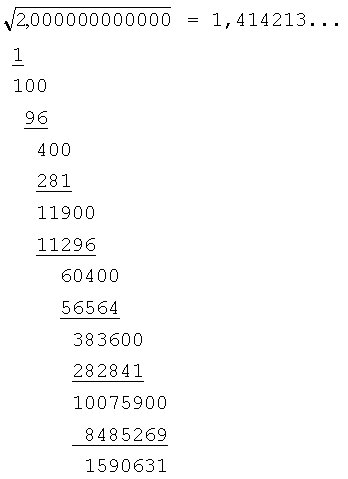
\includegraphics[width=3cm]{2te/reellezahlen/bilder/namenlos.jpg}
\end{minipage}




\section{Rechnen mit Wurzeln}

Generell l\"{a}sst man Wurzeln innerhalb einer Rechnung fast immer
stehen, d.h. man ersetzt z.B. $\sqrt{2}$ nicht durch einen
N\"{a}herungswert der unendlichen Dezimalzahl $1,414213\dots$, sondern
betrachtet das Symbol $\sqrt{2}$ als Abk\"{u}rzung derselben. Wir
d\"{u}rfen also von der (irrationalen) Zahl $\sqrt{2}$ sprechen. Durch
die Multiplikation von $\sqrt{2}$ mit $6$ entsteht so z.B. die
Zahl $6 \sqrt{2}$. Durch anschlie{\ss}ende Addition von $7$ ergibt
sich die Zahl $7+ 6 \sqrt{2}$. Erst als Endergebnis kann man (muss
aber nicht) die ungef\"{a}hre Dezimalzahl anf\"{u}hren: $7+6 \sqrt{2}
\approx 15,48528$


\bs  {\bf Wurzelgesetze} F�r alle $a, b \in \mathbb{R}_0^+$ gilt: 

\bn \item Definitionsmenge von $\sqrt{a}$: $a \in \mathbb{R}^+_0$

\item $\sqrt{a^2}=\left(\sqrt{a}\right)^2=a$ falls $a\geq0$ ist!

\item Addieren und Subtrahieren: (nur {\bf gleiche} Wurzeln!):
$$m\cdot \sqrt{a}\pm n \cdot \sqrt{a}=(m \pm n)\sqrt{a}$$
\item Multiplizieren und Dividieren ($b\neq 0$):
$$\sqrt{a\cdot b}=\sqrt{a} \cdot \sqrt{b} \qquad \qquad \sqrt{\frac{a}{b}}=\frac{\sqrt{a}}{\sqrt{b}}$$

\item Teilweise die Wurzel ziehen:
$$\sqrt{a^2\cdot b}=a \cdot \sqrt{b}$$

\item Nenner rational machen (keine Wurzel im Nenner):

$$\frac{a}{\sqrt{b}}=\frac{a\cdot\sqrt{b}}{\sqrt{b}\cdot \sqrt{b}}=\frac{a\cdot \sqrt{b}}{b}$$


\en\es  

\subsection{Summen (Differenzen) von Wurzeln}
\bb \bt{llll}
 a) & $4\sqrt{2}+\sqrt{2}=(4+1) \sqrt{2}= ......... $ & b) & $-3\sqrt{5}+2\sqrt{5}=(...........) \sqrt{5}=........... $ \\
 c) & $\sqrt{7}-5\sqrt{7}=........$  & d) & $\sqrt{7} -\sqrt{6}=...........$ \et\eb

\subsection{Das Produkt zweier Wurzeln}

\bb \bt{llll}
 a) & $\sqrt{2}\cdot\sqrt{3}=\sqrt{2\cdot 3}=....... $ & b) &
 $\sqrt{2}\cdot\sqrt{8}=......$ \et \eb

Die Wurzel aus einem Produkt kann somit faktorweise gezogen
werden; dies ist einsichtig, wenn man den obigen Satz von "`rechts
nach links"' liest: $\sqrt{a \cdot b}=\sqrt{a}\cdot \sqrt{b}$.

\bb {\tiny .}

\bt{llll}
 a) & $\sqrt{200}=\sqrt{2}\cdot\sqrt{100}=10\sqrt{2}$ & b) & $\sqrt{6400}=\sqrt{64}\cdot\sqrt{100}=....... $ \\
 c) & $\sqrt{81\cdot 10^4}=..... $ &
 & \et\eb

\subsubsection{Achtung!}

Gr\"{o}{\ss}te Vorsicht ist bei folgenden Beispielen geboten:

\bb \label{sddsdgge12} Es ist $ \sqrt{16+9}=\sqrt{25}=5$, \textbf{nicht aber} $
\sqrt{16+9}=\sqrt{16}+\sqrt{9}=4+3=7$. Folglich ist $ \sqrt{16+9} \neq \sqrt{16}+\sqrt{9}$.

Ebenso ist $ \sqrt{100-36}=\sqrt{64}=8$ \textbf{nicht aber}
$\sqrt{100-36}=\sqrt{100}-\sqrt{36}=10-6=4$. Damit gilt auch hier
$ \sqrt{100-36} \neq \sqrt{100}-\sqrt{36}$. \eb

\bme Der obige Satz gilt \textbf{nicht} f\"{u}r Summe und Differenz
d.h. \[ \sqrt{a\pm b} \neq \sqrt{a}\pm \sqrt{b} \quad !!! \] \eme

\bb Vereinfache die folgenden Terme:

\bt{llllll}
 a) & $\sqrt{3}\cdot\sqrt{7}= $ &  b) & $\sqrt{18}\cdot\sqrt{8}= $ &
 c) & $\sqrt{2}\cdot\sqrt{3}\cdot\sqrt{6}= $ \\
 d) & $\sqrt{64}+\sqrt{36}= $ &  e) & $\sqrt{64}\cdot\sqrt{9}= $ &  f) & $\sqrt{\sqrt{36}-\sqrt{4}}=$
 \et  \eb

\subsection{Der Quotient zweier Wurzeln}


\bb Vereinfache:

\bt{llllll}
 a) & $\frac{\sqrt{27}}{\sqrt{3}}=\sqrt{\frac{27}{3}}=\sqrt{9}=\dots $ &
 b) & $\sqrt{8+\frac{1}{4}}=....$ &
 c) & $\frac{\sqrt{24}}{\sqrt{40}}=.... $ \\
 d) & $\sqrt{0,0002}=.... $ & e) & $\sqrt{\frac{7}{3}}\cdot\sqrt{\frac{7}{12}}=.... $ &
 f) & $\frac{\sqrt{3}}{\sqrt{5}}\cdot\frac{\sqrt{10}}{\sqrt{18}}=....$
 \et
\eb



\subsection{Potenzen von Wurzeln}

Auch Potenzen von Wurzeln stellen kein allzu gro{\ss}es Problem
dar:

 \bn\item Quadrate von Wurzeln:

\bb \bt{llll}
 a) & $\sqrt{2}^2=\sqrt{2}\cdot\sqrt{2}= ...... $ & b) & $\sqrt{7,1}^2=....... $ \\
\et \eb

\item H\"{o}here Potenzen:

\bb\bt{llll}
 a) & $\sqrt{13}^3=\sqrt{13}\cdot\sqrt{13}\cdot\sqrt{13}= ....... $ & b) & $\sqrt{7}^4=....... $ \\
\et \eb \en

\ba Berechne:

\bt{llllllll}
 a) & $\sqrt{1,5}^2=$ & b) & $\left( \sqrt{\frac{2}{7}}\right)
 ^4=$ & c) & $(-\sqrt{5})^2=$ & d) & $(-\sqrt{3})^3=$ \et\ea


\subsection{Das teilweise Wurzelziehen}

Die Multiplikationsregel $\sqrt{a \cdot b}=\sqrt{a}\cdot \sqrt{b}$
erlaubt in gewissen F\"{a}llen das sogenannte "`teilweise Ziehen"'
einer Wurzel.

\bb {\tiny .}

\bt{llllll}
 a) & $\sqrt{18}=\sqrt{9\cdot 2}=\sqrt{9}\cdot\sqrt{2}=........ $ &
 b) & $\sqrt{700}=.... $ &  c) & $\sqrt{0,07}=.... $
\et \eb

\bme $ \sqrt{a^2 b}=a\sqrt{b}$ !! \eme

\bb
\[5\sqrt{12}+\sqrt{27}-\sqrt{48}-\sqrt{75}=5\sqrt{4\cdot 3}+\sqrt{9\cdot
3}-\sqrt{16\cdot 3}-\sqrt{25\cdot3}=.......\] \eb

\bme $ -\sqrt{a^2 b}=-a\sqrt{b}$ !! \eme

\subsubsection{Umkehrung:} Genauso kann man, wenn man die beiden obigen
Merks\"{a}tze von rechts nach links liest, einen Faktor vor der Wurzel
in diese "`hineinziehen"'.

\bb Bringe alles unter eine Wurzel:

\bt{llll}
 a) & $2\sqrt{\frac{7}{2}}= .... $ & b) & $-3x\sqrt{\frac{2}{x}}=....$\et
\eb

\ba Versuche teilweise die Wurzel zu ziehen und umzuformen:

\bt{llll}
 a) & $-\sqrt{45}= $ & b) & $4\sqrt{12}(2\sqrt{3}+\sqrt{6})= $ \\
 c) & $\sqrt{\frac{3a^2}{4}}= $ & d) & $\sqrt{c^2+\left(\frac{c}{2}\right)^2}= $ \\
 e) & $\sqrt{x^2 y+x^2 z}= $ &
 f) & $
 \sqrt{8}+\sqrt{12}+\sqrt{18}+\sqrt{48}-\sqrt{72}-\sqrt{108}=$\et\ea


\section{Wiederholung - �bungen}
%\input{smart-reelle.tex}
\ba
\bn 

\item Gibt es f\"{u}r jede reelle Zahl eine Darstellung
$\frac{a}{b}$? Wenn ja, warum; wenn nein, gib ein Gegenbeispiel
an!

\item Warum ist es notwendig, den Zahlenbereich um die reellen Zahlen zu erweitern? Gib ein Beispiel an!

\item Wie bringe ich einen beliebigen Faktor unter die Wurzel? Gib
ein Beispiel an!

\item Richtig oder falsch?

\bt{llllll}
 a) & $-\sqrt{25}=-5$ & b) & $\sqrt{-25}=-5 $ & c) & $\sqrt{36}=6 $ \\
 d) & $-\sqrt{36}=-6 $ & e) & $(-\sqrt{7})^2 =-7 $ & f) & $(-\sqrt{7})^2=7 $ \et



\item Wo ist der Fehler?

\begin{eqnarray*}
1-\sqrt{2}=\sqrt{(1-\sqrt{2})^2}&=&\sqrt{(\sqrt{2}-1)^2}=\sqrt{2}-1\\
1-\sqrt{2}&=&\sqrt{2}-1\\
2& = & 2\sqrt{2}\\
1& = & \sqrt{2}\\
1& = & 2\\
\end{eqnarray*}

\item Berechne:

\bt{llllll}
 a) & $\sqrt{32}\cdot\sqrt{50} $ &  b) & $\sqrt{3a^2 b^3}\cdot\sqrt{24bc^2} $ &
 c) & $\sqrt{75}:\sqrt{27} $ \\
 d) & $\frac{\sqrt{3x^2 y^5}}{\sqrt{x y^3}} $ &  e) & $(3\sqrt{5}-5\sqrt{3})\sqrt{15} $ &
 f) & $\sqrt{72}\cdot\sqrt{3}\cdot\sqrt{6} $ \\
 g) & $\frac{3\sqrt{5}+5\sqrt{3}}{\sqrt{15}} $ &  h) & $\sqrt{\frac{10}{7}}\cdot \sqrt{\frac{21}{15}}\cdot\sqrt{18} $ &
 i) & $\frac{\sqrt{33}}{\sqrt{10}}\cdot\sqrt{\frac{3}{7}}\cdot\sqrt{\frac{14}{4}}\cdot\sqrt{33} $
\et

\item Bringe den wurzelfreien Faktor unter die Wurzel und vereinfache:

\bt{llllll}
 a) & $7\sqrt{\frac{5}{7}} $ &  b) & $8\sqrt{\frac{22}{128}} $ &  c) & $x\sqrt{x^3} $ \\
 d) & $-x^2 \sqrt{\frac{1}{x^3}} $ &  e) & $\frac{1}{x}\sqrt{x^2} $ &  f) & $\frac{z^2}{\sqrt{3z^2}} $
\et

\item Vereinfache durch teilweises Wurzelziehen:

\bt{llll}
 a) & $\sqrt{27} $ & b) & $\sqrt{\frac{169ab^4 c^2}{32}} $ \\
 c) & $\sqrt{\frac{48}{27}} $ & d) & $\sqrt{20}+\sqrt{45}-\sqrt{80}-\sqrt{5} $ \\
 e) & $\sqrt{16x+32y} $ & f) & $3\sqrt{48}-5\sqrt{75}-2\sqrt{12}+7\sqrt{27} $ \\
 g) & $\sqrt{3r^2 -2r^4 s} $ & h) & $12\sqrt{98}+4\sqrt{8}-10\sqrt{50}-14\sqrt{72}+8\sqrt{32}+6\sqrt{8} $
\et 


\item
Bestimme mit dem Heron-Verfahren den Wert von $\sqrt{7}$ auf 6 Dezimalen genau.W"ahle dazu
als Startwert $x=1$.
\item
Untersuche, ob $x$ rational ist! Schreibe zu jeder Antwort eine kurze, aber logisch einwandfreie
Begr"undung! Falls $x$ rational ist, ist $x$ als vollst"andig gek"urzter Bruch darzustellen!
\begin{enumerate}
\item $x = 2,314113111411113111114.......$
\item $x = -0,0545454.......$
\item $x = 0,12636363.......$
\item $x^2 = 21$
\item $x^2 = -4$
\end{enumerate}
\item
 Gib die ersten f"unf Intervalle einer Intervallschachtelung f"ur $3,461057...$ an.

\item
Berechne mit der Halbierungsmethode eine Intervallschachtelung f"ur $\sqrt{11}$!\\
Starte mit dem Intervall $I_0$ (Intervall"ange 1), das nat"urliche Zahlen als
Grenzen hat und brich ab, wenn die Intervall"ange kleiner als 0,1 ist!\\
Wie oft mu"s halbiert werden, wenn als Abbruchbedingung die Intervall"ange 0,00001 steht?

\item
 Welche der folgenden Intervalle bilden {\bf nicht} den Beginn einer Intervallschachtelung,
wenn man sinngem"a"s fortsetzt? Begr"unde kurz.
\begin{enumerate}
\item
$[4;5]$, $[4,8;5]$, $[4,89;5]$, $[4,899;5]$, \dots
\item
$[7;8]$, $[7,7;7,8]$, $[7,77;7,78]$, $[7,777;7,778]$ \dots
\item
$[{2\over3};1]$, $[{2\over5};{1\over 2}]$, $[{2\over7};{1\over 3}]$, $[{2\over9};{1\over 4}]$,
$[{2\over11};{1\over 5}]$ \dots
\end{enumerate}
\item
Welche Gleichung der Form $x^2=a$ hat als L"osung

(a)\qquad $-2$~ ?\hspace{2cm} (b)\qquad $ \frac{1}{\sqrt{5}}$~? 
\item
 Bestimme die Definitionsmenge von:
\begin{enumerate}
\item
$\sqrt{c + 4}$
\item
$\sqrt{-c^2}$
\item
$\sqrt{(- c)^2}$
\item
$\sqrt{c^3}$
\end{enumerate}
\item
Sind die folgenden Aussagen wahr oder falsch? Gib gegebenenfalls an, was zus"atzlich vorausgesetzt
werden mu"s, damit die Aussagen wahr werden.
\begin{enumerate}
\item
Ist $0 < x < y $, so ist $\sqrt{x} < \sqrt{y}$
\item
Es gilt stets $\sqrt{x} < x$.
\item
$\left( \sqrt{-x}\right)^2 = \sqrt{x^2}$
\end{enumerate}
\item
Bestimme die Definitionsmenge des folgenden Terms:
\[\sqrt \frac{-2}{x\cdot(x-4)}\]
\item
 Vereinfache und radiziere soweit wie m"oglich:
\begin{enumerate}
\item
$\sqrt{16 x^2 + 56 x + 49}$
\item
$\sqrt{\sqrt{81c^2}}$
\item
$\sqrt{0,00000175}$
\item
$\left(\sqrt{\frac{  1}{  a^3}} \cdot \sqrt{\frac{  b^6}{  c}} \right) : \sqrt{\frac{  bc}{ 
a^4}}$
\item
$3\sqrt{75} + \sqrt{147} - 4 \sqrt{27} - \sqrt{3}$
\end{enumerate}
\item
Radiziere und vereinfache so weit wie m"oglich:
$$
\sqrt{4a^2} - \sqrt{a^2-4a+4}, \ \ (a<0)
$$
\item
Vereinfache:
$$
\sqrt{275} + \sqrt{343} - \sqrt{112} - \sqrt{99}
$$
\item
Radiziere und vereinfache soweit wie m"oglich:
$$
\sqrt{27a^3+81a^2b \over {(a+3b)}^3},\quad a,b>0
$$
\item
 Vereinfache soweit wie m"oglich:
$$
\sqrt{4a^2\cdot(x-3) \over (x+3)} \cdot \sqrt{(x^2-9)\cdot a^2}; \quad x<-3
$$
\item
Radiziere so weit wie m"oglich und bestimme jeweils zus"atzlich die Bedingungen an die Variablen,
damit der Term definiert ist:
\begin{enumerate}
\item   $\sqrt{(-4)^2x^{14}y^{27}z^{7}}$
\item   $\sqrt{a^4b^3-a^4b^2}$
\end{enumerate}

\item
Radiziere, gegebenenfalls mit Fallunterscheidung:
\[\sqrt{4x^2+64-32x}\]
\item
Gib an, f"ur welche Werte der Variablen die folgenden Wurzelterme definiert sind und radiziere dann
so weit wie m"oglich:
\[\mbox{(a)}~~\sqrt\frac{x^5y^2}{z^4}\hspace{3cm}
\mbox{(b)}~~\sqrt\frac{(a^2+2)\cdot b^3}{c^2-8c+16}\]
\item
 Stelle rationale Nenner her und vereinfache soweit wie m"oglich:
\begin{enumerate}
\item
$\frac{  240}{  \sqrt{180}}$
\item
$\frac{  9 \sqrt{2}}{  \sqrt{98} + \sqrt{72}}$
\end{enumerate}
\item
Mache den Nenner rational und vereinfache soweit wie m"oglich:
$$
3+ 2\sqrt{3} \over 3 -\sqrt{3}
$$
\en
\ea

\section{Wurzelgleichungen}
\bd  Tritt in einer Gleichung die Unbekannte mindestens einmal unter einer Wurzle auf, so nennt sie {\bf Wurzelgleichung}. Dabei beschr�nken wir uns hier auf Quadratwurzeln.\ed  

\bme \bn \item {\bf Gleichung potenzieren!}

Eine Wurzelgleichung l�st man durch Potenzieren (eine Quadratwurzelgleichung durch quadrieren). 

Dabei soll die Gleichung so umgeformt werden, dass die Wurzel isoliert (also alleine) auf einer Seite der Gleichung steht und anschlie�end die beiden Seiten der Gleichung mit dem Wurzelexponenten potenziert. Falls n�tig, wiederholt man dieses Verfahren, bis alle Wurzeln eliminiert sind.

\item {\bf Probe Pflicht!}

Das Potenzieren einer Gleichung ist KEINE �quivalenzumformung, folglich kann sich die gesuchte L�sungsmenge �ndern. Ein solcher Rechenschritt kann n�mlich aus einer falschen Aussage wie $2=-2$ eine wahre Aussage $(2^2=(-2)^2)$ machen. Daher k�nnen beim Potenzieren "`Scheinl�sungen"' hinzukommen, die keine L�sungen der urspr�nglichen Gleichung sind. Die Probe ist daher unverzichtbar!
\en 
\eme 

\ba Bestimme jeweils die Definitions- und die L�sungsmenge:
$$\begin{array}{lll}
a) \quad \sqrt{x}=1 & b) \quad \sqrt{x+7}=-4 & c) \quad \sqrt{x-1}+10=12\\
d) \quad \sqrt{x+30}=6\sqrt{x-5} & e) \quad 2\sqrt{x+1}=\sqrt{x+13} & f) \quad \sqrt{x}=\sqrt{x+8}-2\\
g) \quad \sqrt{x-4}-\sqrt{x+11}+3=0 & h) \quad \sqrt{8-2x}=1+\sqrt{5-x} & i) \quad \sqrt{x-10}+\sqrt{x+10}=10\\
j) \quad \sqrt{2x-\sqrt{7x+4}}=\sqrt{3x+2} & k) \quad \sqrt{x+1}+x=5 & l) \quad \sqrt{x-5}\cdot\sqrt{x+3}=x \\
m) \quad \sqrt{13x+12}=2\sqrt{x-3}+3\sqrt{x} & n) \quad \sqrt{4x-9}+\sqrt{6x-7}=&\sqrt{5x-3}+\sqrt{5x-13}  \\
\end{array}$$

\ea


\ba {\bf mit L�sungen} \begin{eqnarray}
\begin{array}{llc@{\qquad}r}
1)&\quad \sqrt{x}-\sqrt{2x+1}=-1        & &[0;4]\\%[0.4cm]
2)&\quad \sqrt{3x-5}-\sqrt{2x-5}=1      & &[3;7]\\%[0.4cm]
3)&\quad \sqrt{3x+1}+\sqrt{x-4}=\sqrt{4x+5} & &[5]\\%[0.4cm]
4)&\quad \sqrt{2x+2}=2+\sqrt{3x+15}         & &[\{ \}]\\%[0.4cm]
5)&\quad \D{\frac{\sqrt{x^2-16}}{\sqrt{x-3}}}+\sqrt{x+3}=
    \D{\frac{7}{\sqrt{x-3}}}        & &[5]\\%[0.4cm]
%\end{array}
%\eeq
%\beq
%\begin{array}{llc@{\qquad}r}
6)&\quad\sqrt{2x-3}-\sqrt{x+2}=1        & &[14]\\%[0.4cm]
7)&\quad\sqrt{x^2+16}-\sqrt{6x+7}=3-x       & &[-\frac{7}{6};3]\\%[0.4cm]
8)&\quad\sqrt{3x+1}+\sqrt{x-4}=\sqrt{4x+5}  & &[5]\\%[0.4cm]
9)&\quad\sqrt{4x-11}-\sqrt{21-4x}=2\sqrt{x-4}   & &[4;5]\\%[0.4cm]
10)&\quad\sqrt{4x-3}-\sqrt{13-4x}=2\sqrt{x-2}   & &[2;3]\\%[0.4cm]
11)&\quad\sqrt{3x^2+21}+\sqrt{x^2+3}=2\sqrt{x^2+18} & &[\pm 3]\\%[0.4cm]
12)&\quad\sqrt{x-4}=\sqrt{x-9}-\sqrt{x-1}   & &[\{\}]\\%[0.4cm]
13)&\quad\sqrt{3-4x}+\sqrt{1+9x}=\sqrt{4+5x}    & &[\frac{3}{4};-\frac{1}{9}]\\%[0.4cm]
14)&\quad\sqrt{2x+8}-\sqrt{x+5}=7       & &[284]\\%[0.4cm]
\end{array}
 \end{eqnarray}  \begin{eqnarray}
\begin{array}{llc@{\qquad}r}
15)&\quad2\sqrt{x+3a^2}-5a=\sqrt{x-5a^2}    & &[\frac{94a^2}{9},6a^2]\\%[0.4cm]
16)&\quad\sqrt{x-2}=\sqrt{4x+1}-\sqrt{x+3}  & &[6]\\%[0.4cm]
17)&\quad\sqrt{3x-6}+\sqrt{2x+4}=2\sqrt{x}  & &[2]\\%[0.4cm]
18)&\quad\sqrt{x+2}+\sqrt{x-3}=\sqrt{3x+4}  & &[7]\\%[0.4cm]
19)&\quad2\sqrt{3x+1}+3\sqrt{5x-4}=4\sqrt{6x+1} & &[8]\\%[0.4cm]
20)&\quad\sqrt{9x^2+b^2}-3x=\sqrt{b^2-6x}   & &[0,\frac{b^2-1}{6}]\\%[0.4cm]
\end{array}
 \end{eqnarray}
\ea 


 
 \chapter{Die quadratische Funktion}
%\paragraph*{Einstieg: Stationenunterricht}
%In den Pflicht- und Wahl/Pflichtstationen wurden die wichtigen Inhalte zum Thema erarbeitet. Im Kapitel \ref{zufquadfkt} wird das %Wesentliche zusammengefasst.


\bd  Eine {\bf quadratische Funktion} (auch ganzrationale Funktion 2. Grades oder Polynom 2. Grades) ist eine Funktion, die als Funktionsterm ein Polynom vom Grad 2 besitzt, also von der Form

    $$f(x) = ax^2 + bx + c \qquad \mbox{(mit }a \neq 0)$$

ist. Der Graph ist eine {\it Parabel}. F�r $a = 0$ ergibt sich eine lineare Funktion.\ed 

Zun�chst die Frage: welche Rolle spielen die Koeffizienten $a, b$ und $c$. Dazu zwei �bungen im Computerraum:

\ba \bn \item Computerraum: Die quadratische Funktionen

Die Arbeitsanweisungen m�ssen \textbf{genauestens gelesen} werden.
Alle Beobachtungen sind in \textbf{ganzen S�tzen} festzuhalten!

Verwende eine Tabellenkalkulation und ein Textverarbeitungsprogramm.
�ffne die Datei \texttt{DynABQuadratischeFunktion.xls} Sie
enth�lt zwei Arbeitsbl�tter mit den Namen "`Scheitelform"' und
"`allgemeine Form"'. Mit der Maus k�nnen die Konstanten $a,d,e$
der Scheitelform $y=a(x+d)^2+e$ bzw. $a,b,c$ der allgemeinen Form
$y=ax^2+bx+c$ ge�ndert werden; die Funktion selbst ver�ndert sich
automatisch mit.

Textverarbeitung-�berschrift:
"`Arbeitsblatt - Quadratische Funktionen"'; Kopfzeile: dein Name.





\begin{enumerate}

\item Wechsle in der Excel- Datei zum Arbeitsblatt "`Scheitelform"'. 
Erstelle  eine kleinere �berschrift
\textbf{"`Scheitelform: $y=a(x+d)^2+e$"'} und bearbeite die
folgenden Fragen:

\begin{enumerate}

\item Stelle zun�chst f�r die Konstanten (falls nicht schon
eingestellt) folgende Werte ein: $a=1,d=0,e=0$. �ndere nun mit der
Maus den Wert f�r $a$. Beobachte, was sich genau ver�ndert und
halte deine Beobachtungen fest!

\item Setze $a$ wieder auf den Wert $1$. Ver�ndere nun den Wert
$d$ und halte wie oben deine Beobachtungen fest!

\item Setze $d$ auf den Wert $0$. Ver�ndere nun den Wert $e$ und
halte deine Beobachtungen fest!

\item Versuche (evtl. mit Hilfe verschiedener selbst gew�hlter
Werte) eine allgemeine Formel f�r den Scheitelpunkt $S$ ($=$
h�chster oder tiefster Punkt der Kurve) in Abh�ngigkeit der
Parameter $a,d,e$ zu finden!

\end{enumerate}

\item Wechsle in der Excel- Datei zum Arbeitsblatt "`Allgemeine
Form"'. Erstelle 
 eine kleinere �berschrift
\textbf{"`Allgemeine Form: $y=ax^2+bx+c$"'} und bearbeite die
folgenden Fragen:

\begin{enumerate}

\item Stelle zun�chst f�r die Konstanten (falls nicht schon
eingestellt) folgende Werte ein: $a=1,b=0,c=0$. �ndere nun mit der
Maus den Wert f�r $a$. Beobachte, was sich genau ver�ndert und
halte deine Beobachtungen fest!

\item Setze $a$ wieder auf den Wert $1$. Ver�ndere nun den Wert
$b$ und halte wie oben deine Beobachtungen fest! Betrachte
insbesondere die Lage der Nullstellen.

\item Setze $b$ auf den Wert $0$. Ver�ndere nun den Wert $c$ und
halte deine Beobachtungen fest!

\item Versuche (evtl. mit Hilfe verschiedener selbst gew�hlter
Werte) eine allgemeine Formel f�r den $x-$Wert des Scheitelpunkts
$S$ ($x_{S}$) in Abh�ngigkeit der Parameter $a,b,c$ zu finden!

\end{enumerate}

\item �berpr�fe, ob �berall \textbf{ausf�hrlich in ganzen S�tzen}
geantwortet wurde. Versuche schlie�lich die Antworten auf obige
Fragen auf eine Seite (maximal zwei) zu bringen und in einer
ansehnlichen Form darzustellen. Drucke die Seite(n) aus!

\item \textbf{F�r all jene, die fr�her fertig werden:} Versuche
mit Hilfe der Excel- Datei auf den beiden Arbeitsbl�ttern
Funktionen mit denselben Graphen ausfindig zu machen. Vergleiche
die jeweiligen Funktionsvorschriften und �berlege dir, wie man
eine Funktionsgleichung in Scheitelform in die allgemeine Form
umrechnen k�nnte und umgekehrt!

\end{enumerate}
\item Computerraum: Zeichne mit Geonext drei Schieberegler f�r die Parameter $a$, $b$ und $c$. (evtl. Strecken von $-5$ bis $5$). Zeichne den Funktionsgraphen in Abh�ngigkeit dieser Gleiter und beobachte ihren Einfluss auf den Graphen.

\en 
\ea 





\section{Eigenschaften der quadratischen Funktion - Scheitelpunktform}\label{zufquadfkt}
\bme 
\begin{description}
\item[Die quadratische Funktion $y=x^2$]:

	\begin{minipage}{11cm}
	\bi
	\item Definitionsmenge $D=\mathbb{R}$
	\item Wertemenge $W=\mathbb{R}^+$
	\item der Graf ist eine {\bf Parabel}
	\item der Graf ist achsensymmetrisch bez�glich der $y$-Achse
	\item ber�hrt die $x$-Achse im Ursprung - Scheitel der Parabel: $S(0|0)$
	\ei 
	\end{minipage} 
	\begin{minipage}{3cm}
	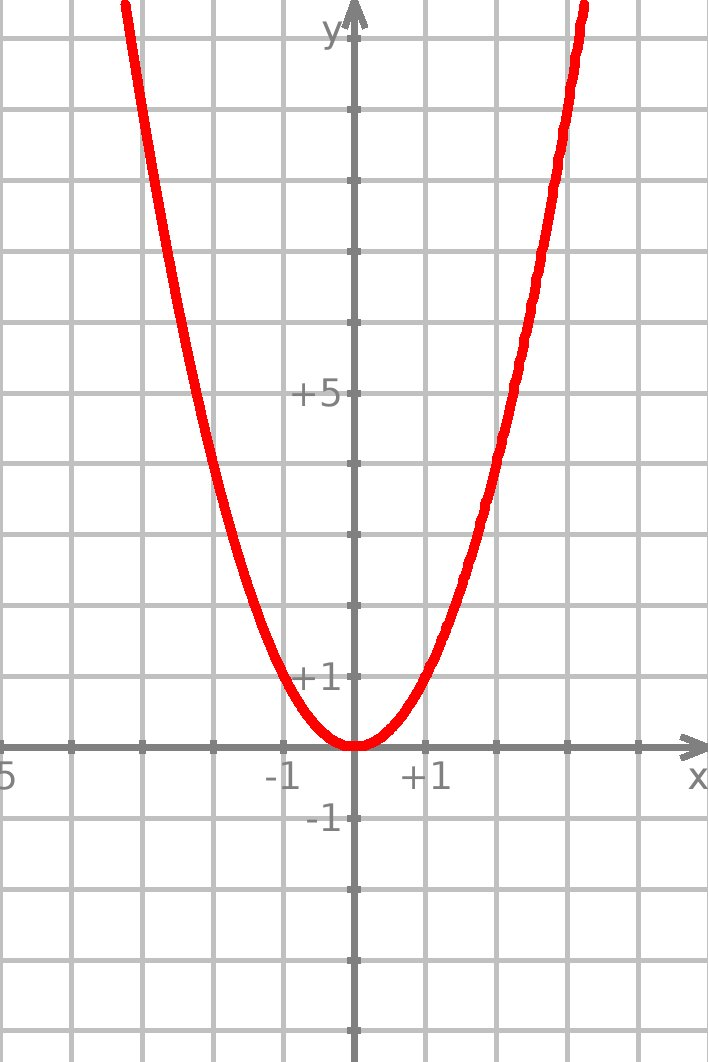
\includegraphics[width=3cm]{2te/quadratischefunktion/bilder/reinquadfkt2.jpg}
	\end{minipage}


\item[Die quadratische Funktion $y=ax^2$]:

	\begin{minipage}{11cm}
	\bi
		\item der Graf ist eine {\bf Parabel}, sie ist 
	\bi \item nach oben ge�ffnet, falls $a>0$ ist
		\item nach unten ge�ffnet, falls $a<0$ ist
		\item keine quadratische Funktion ($y=0$), falls $a=0$ ist.
	\ei

	\item Sie entsteht, indem man die Grundparabel in Richtung der $y$-Achse
		\bi \item {\it streckt}, falls $|a|>1$ ist (sie ist dann steiler als die Grundparabel)
		\item  {\it staucht}, falls $|a|<1$ ist (sie ist dann flacher als die Grundparabel)
		\item und sie, falls $a<0$, anschlie�end noch an der $x-Achse$ spiegelt.
		\ei 
		Welche Grafen sind rechts gezeichnet?
	
		$..............$ $..............$. $.................$
	\item der Graf ist achsensymmetrisch bez�glich der $y$-Achse
	\item ber�hrt die $x$-Achse im Ursprung - Scheitel der Parabel: $S(0|0)$
	\ei 
	\end{minipage} 
	\begin{minipage}{3cm}
	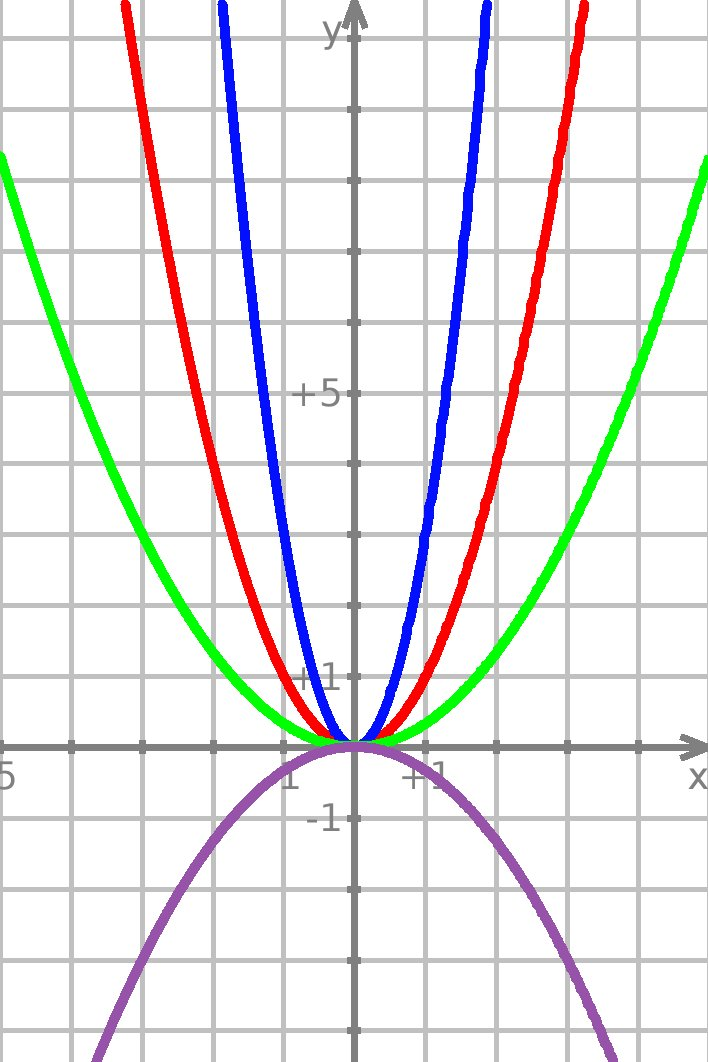
\includegraphics[width=3cm]{2te/quadratischefunktion/bilder/reinquadfkt3.jpg}
	\end{minipage}


\item[Die quadratische Funktion $y=a(x-d)^2$]:

	\begin{minipage}{11cm}
	Der Graf dieser quadratischen Funktion ist eine Parabel mit dem Scheitel $S(d|0)$ auf der $x$-Achse. Sie entsteht durch eine Horizontalverschiebung (entlang der $x$-Achse) der Parabel $y=ax^2$ um $d$ Einheiten (nach rechts, falls $d$ negativ ist, nach links, falls $d$ positiv ist).

	Welche Funktionsgrafen sind rechts gezeichnet?

	$................$ $...................$
	\end{minipage} 
	\begin{minipage}{3cm}
	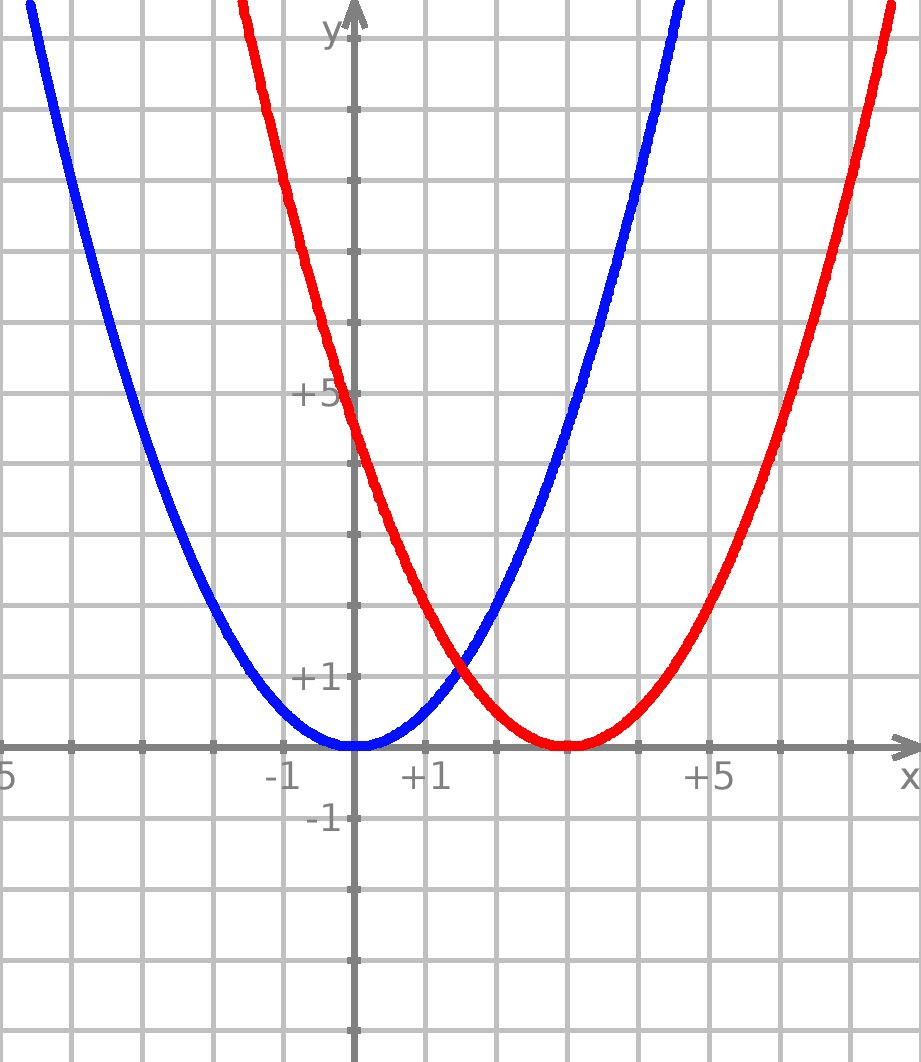
\includegraphics[width=3cm]{2te/quadratischefunktion/bilder/allgquadfthorizontaleverschiebung.jpg}
	\end{minipage}


\item[Die quadratische Funktion $y=ax^2+e$]:

	\begin{minipage}{11cm}
	Der Graf dieser quadratischen Funktion ist eine Parabel mit dem Scheitel $S(0|e)$ auf der $y$-Achse. Sie entsteht durch eine Vertikalverschiebung (entlang der $y$-Achse) der Parabel $y=ax^2$ um $e$ Einheiten (nach oben, falls $e$ positiv ist, nach unten, falls $e$ negativ ist).

	Welche Funktionsgrafen sind rechts gezeichnet?

	$................$ $...................$
	\end{minipage} 
	\begin{minipage}{3cm}
	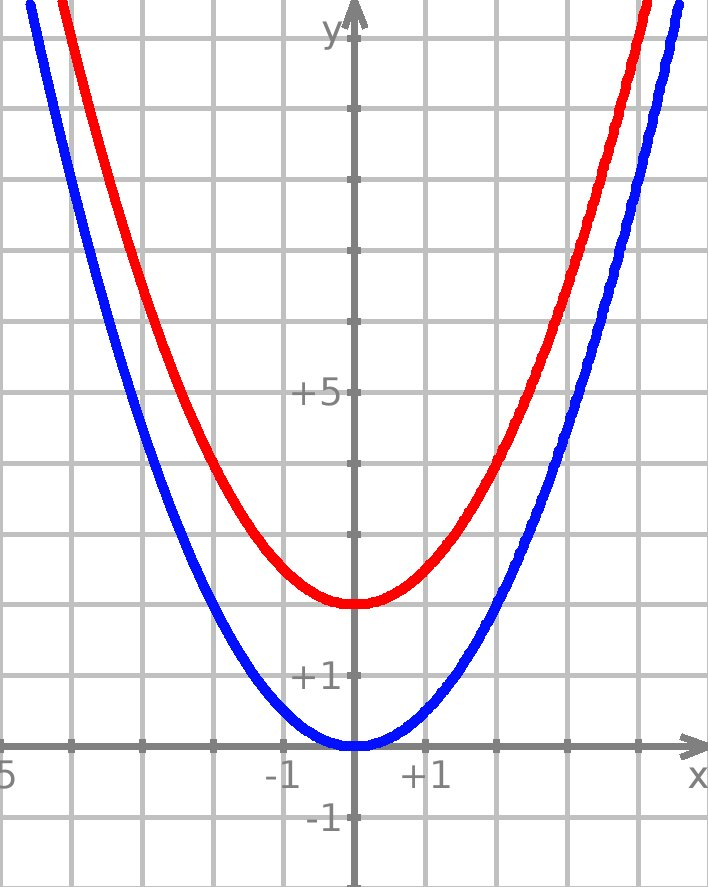
\includegraphics[width=3cm]{2te/quadratischefunktion/bilder/allgquadftvertikaleverschiebung.jpg}
	\end{minipage}

\item[Die quadratische Funktion $y=a(x-d)^2+e$ (Scheitelpunktform)]:

	\begin{minipage}{11cm}
	Der Graf dieser quadratischen Funktion ist eine Parabel mit dem Scheitel $S(d|e)$. Sie entsteht durch eine Horizontal- und eine Vertikalverschiebung  der Parabel $y=ax^2$.

	Welche Funktionsgrafen sind rechts gezeichnet?

	$................$ $...................$
	\end{minipage} 
	\begin{minipage}{3cm}
	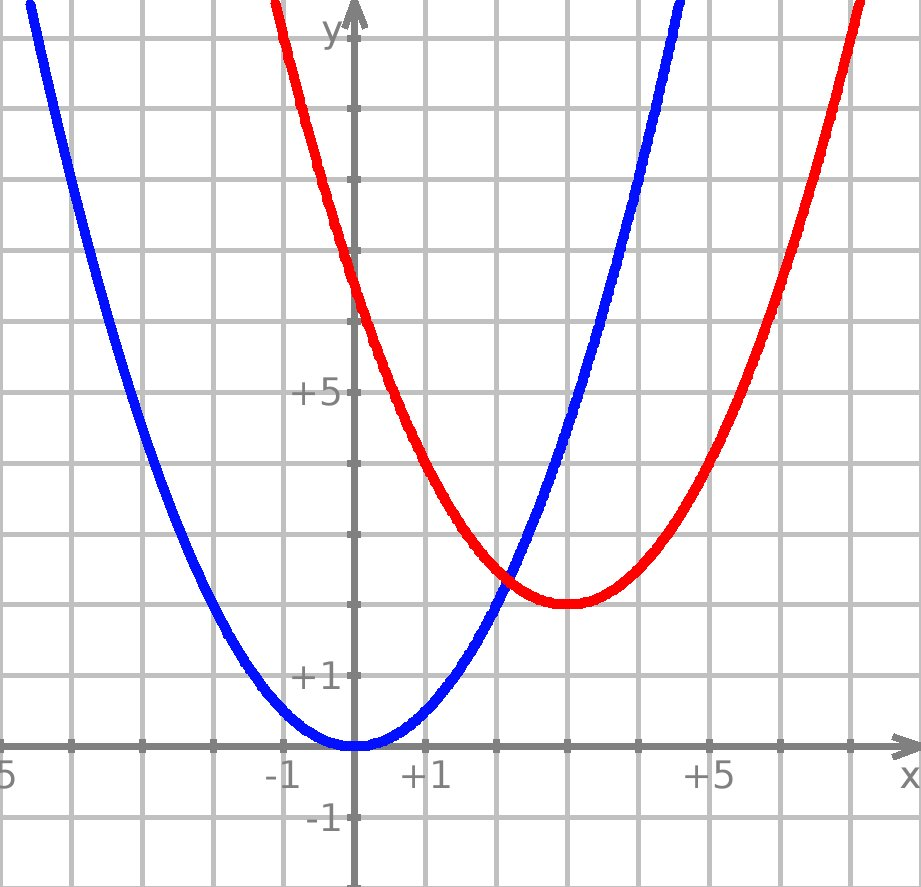
\includegraphics[width=3cm]{2te/quadratischefunktion/bilder/allgquadfthorizontaleundvertikaleverschiebung.jpg}
	\end{minipage}


\item [Die allgemeine quadratische Funktion $y=ax^2+bx+c$]:
	
	\begin{minipage}{11cm}
	$ax^2$ nennt man quadratisches Glied, $bx$ lineares Glied und $c$ hei�t absolutes Glied.

	Bringt man die quadratische Funktion $y=ax^2+bx+c$ durch quadratische Erg�nzung auf die Scheitelpunktform $y=a(x-d)^2+e$, so ergeben sich die Koordinaten des {\bf Scheitels} $$S\left(-\frac{b}{2a}|\frac{4ac-b^2}{4a}\right)$$

	Der Graf entsteht also aus dem Graphen der Parabel $y=ax^2$ durch eine Horizontal- (um $d$-Einheiten) und eine Vertikalverschiebung (um $e$-Einheiten).

	
	

	Welche Funktionsgrafen sind rechts gezeichnet?

	$................$ $...................$
	\end{minipage} 
	\begin{minipage}{3cm}
	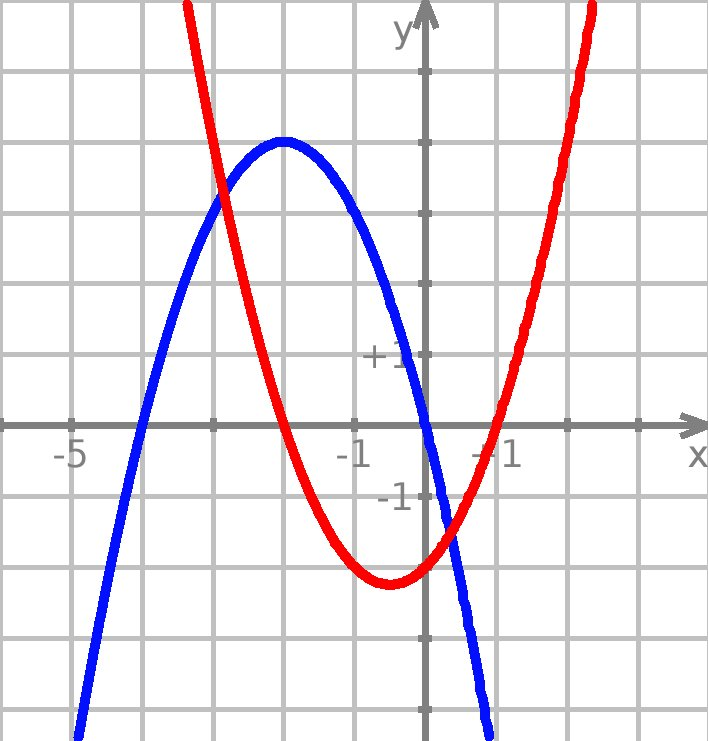
\includegraphics[width=3cm]{2te/quadratischefunktion/bilder/allgquadfkt9.jpg}
	\end{minipage} 



\end{description}
\eme 

\section{Die Nullstellen der quadratischen Funktion - die quadratische Gleichung}

Sucht man die Nullstellen einer Funktion, so setzt man die Funktionsgleichung gleich Null und l�st die entsprechende Gleichung. Bei einer quadratischen Funktion ergibt sich dabei die sog. quadratische Gleichung.

\bd Eine {\bf quadratische Gleichung} hat die Form $$ax^2 +bx+c=0$$ oder kann auf diese Form gebracht werden.\ed 

\bs  Die quadratische Gleichung kann mit Hilfe der Formel $$x_{1/2}=\frac{-b\pm \sqrt{b^2-4ac}}{2a}$$ gel�st werden. Dabei nennt man den Ausdruck $b^2-4ac$ auch Diskriminante (lat. {\it discriminare} = unterscheiden)  und bezeichnet ihn mit $D$.\es 

\begin{proof}
Die Formel kannmit Hilfe der quadratischen Erg�nzung bewiesen werden: ... 
\end{proof}

\bme  
	\begin{itemize}
		\item Die reinquadratische Gleichung $x^2=d$:

		\begin{minipage}{10cm}Die {\bf reinquadratische Gleichung} hat die Form $$x^2=d$$ oder l�sst sich auf diese Form bringen. Es gilt:
		\bi \item F�r $d>0$ gibt es zwei L�sungen $x_1=+\sqrt{d}$ und $x_2=-\sqrt{d}$
		\item F�r $d=0$ gibt es eine L�sung $x=0$
		\item F�r $d<0$ gibt es keine L�sung $\mathbb{L}=\{ \}$
		\ei
		Rechts Geometrische Interpretation: die Funktion $y=x^2+d$ hat keine, eine oder zwei Nullstellen. Welche Funktionsgrafen sind gezeichnet?\\
		..............      ..............      ..............
		\end{minipage} 
		\begin{minipage}{3cm}
		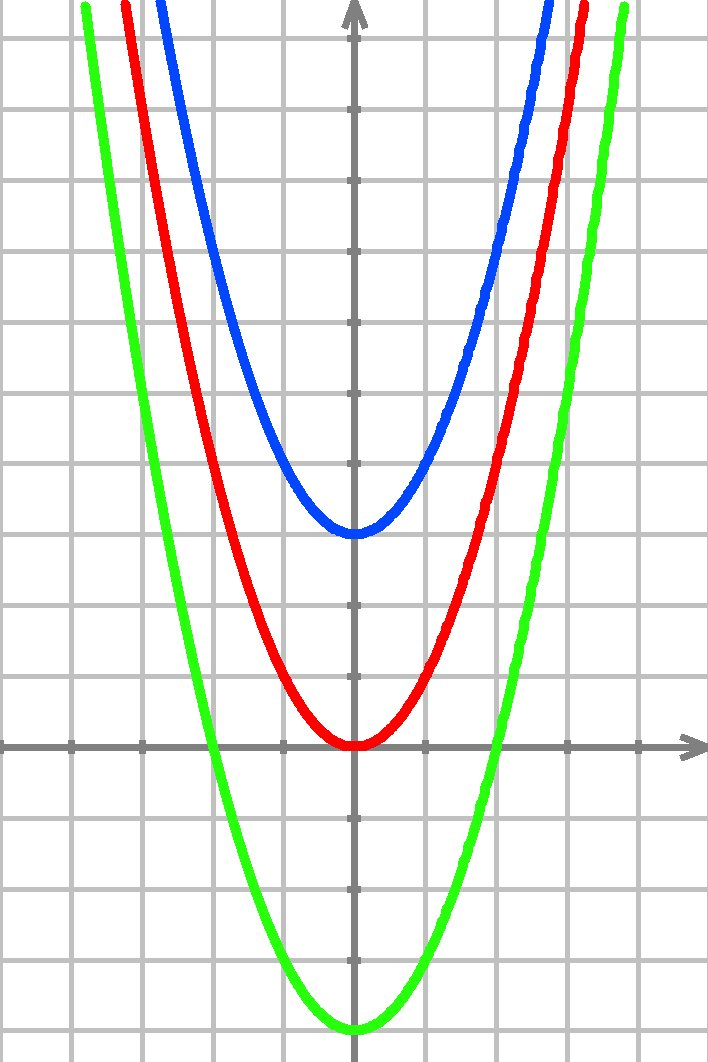
\includegraphics[width=3cm]{2te/quadratischefunktion/bilder/reinquadfkt.jpg}
		\end{minipage}

		\item Die allgemeine quadratische Gleichung $ax^2+bx+c=0$

		\begin{minipage}{10cm}Bei der {\bf allgemeinen quadratischen Gleichung} $$ax^2+bx+c=0$$ h�ngt die L�sung von der {\bf Diskriminante} $$D=b^2-4ac$$ ab:
		\bi \item F�r $D>0$ gibt es zwei L�sungen\\ $x_1=\frac{-b+\sqrt{D}}{2a}$ und $x_2=\frac{-b-\sqrt{D}}{2a}$
		\item F�r $D=0$ gibt es eine L�sung $x=-\frac{b}{2a}$
		\item F�r $D<0$ gibt es keine L�sung $\mathbb{L}=\{ \}$
		\ei
		Rechts: Geometrische Interpretation: die Funktion $y=ax^2+bx+c$ hat keine, eine oder zwei Nullstellen. Welche Funktionsgrafen sind gezeichnet?\\
		..............      ..............      ..............
		\end{minipage} 
		\begin{minipage}{3cm}
		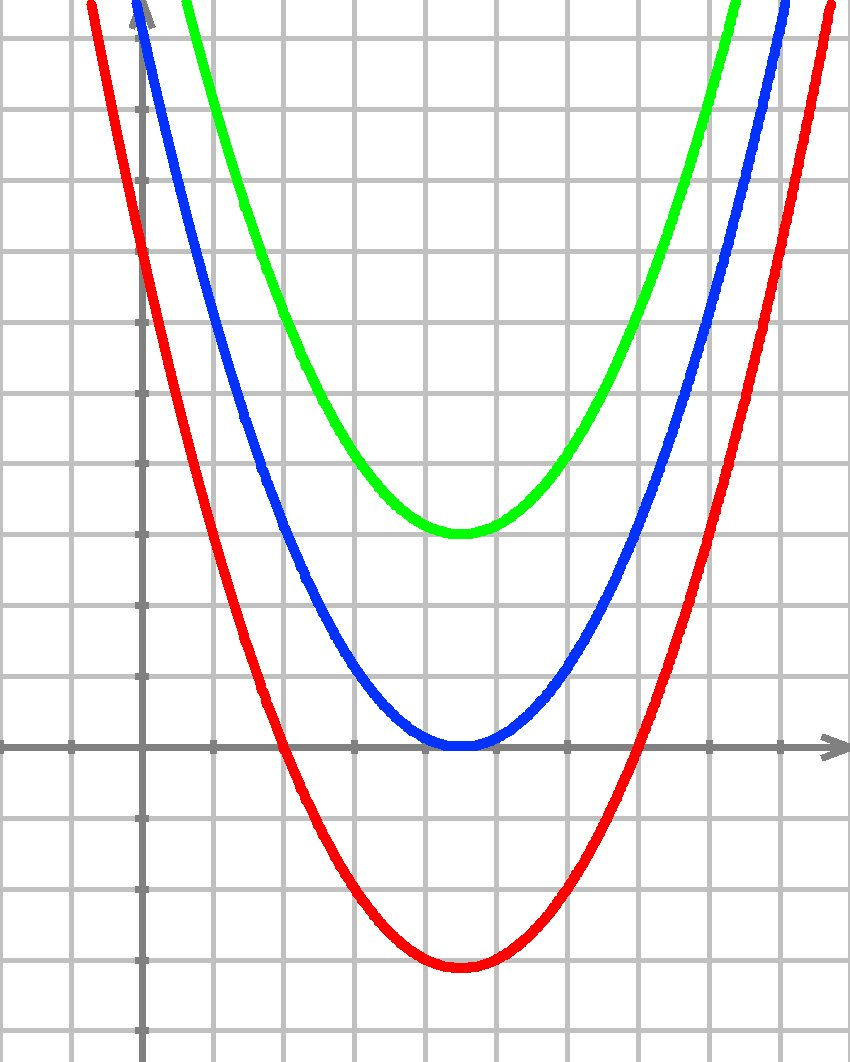
\includegraphics[width=3cm]{2te/quadratischefunktion/bilder/allgquadfkt.jpg}
		\end{minipage}
		
		\item Die Zerlegung von quadratischen Polynomen

		Jedes quadratische Polynom $ax^2+bx+c$ mit positiver Diskriminante (die entsprechende Funktion hat also $2$ Nullstellen $x_1$ und $x_2$) kann in ein Produkt von Linearfaktoren zerlegt werden: $$ax^2+bx+c=a(x-x_1)(x-x_2)$$
	\end{itemize}
\eme 

\section{Zusammenfassung: quadratische Gleichungen}

\bs
Eine Gleichung der Form: $ax^2+bx+c=0$ hei{\ss}t {\bf Normalform} der quadratischen
Gleichung. (Der Grad der Gleichung ist gleich dem
Exponenten der Variablen) \\
Die L\"{o}sung der quadratischen Gleichung berechnet sich aus: 
\begin{eqnarray}
x_{1,2}=\frac{-b\pm\sqrt{b^2-4ac}}{2a} \end{eqnarray}
 der Wert $D=b^2-4ac$ unter der Wurzel
hei{\ss}t {\bf Diskriminante}  und gibt an, ob die Gleichung zwei L\"{o}sungen $(D>0)$, genau
eine L\"{o}sung $(D=0)$, oder
keine L\"{o}sung $(D<0)$ besitzt.\\
Besitzt eine quadratische Gleichung zwei L\"{o}sungen $x_1,x_2$ kann sie auf folgende Art
in Faktoren zerlegt werden: \begin{eqnarray}
ax^2+bx+c=a(x-x_1)(x-x_2), \quad \mbox{mit} \quad
 c= ax_1x_2  \end{eqnarray}
Besitzt sie genau eine L\"{o}sung, n\"{a}mlich $-\frac{b}{2a}$ ist die Zerlegung:
$ax^2+bx+c=a(x+\frac{b}{2a})^2$, $c$ entspricht dann dem Wert, $\frac{b^2}{4a}$, wie
durch einfaches Ausmultiplizieren leicht ersichtlich
wird.
\es


\begin{center}
\begin{figure}[hbt]
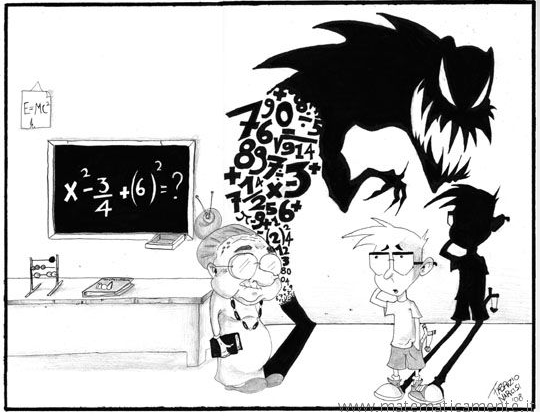
\includegraphics[width=5cm]{2te/quadratischefunktion/bilder/quadratischehexe.png}
\caption{Quadratische Gleichungen machen Lehrer noch nicht zu Monstern ...}
\end{figure}
\end{center}

\ba
\bn \item $  (9+x)(7-x)+(9-x)(7+x)=76$ \hfill (L�sung: $ [\pm 5] $)
\item $  (x+9)^2=2(x+7)^2-17$ \hfill (L�sung: $ [0,-10] $)
\item $ \D{\frac{a+1}{a-1}}x=\D{\frac{x^2+x}{x-1}}  $ \hfill (L�sung: $ [0,a] $)
\item $ (x+a)^2+2ax=a^2  $ \hfill (L�sung: $ [0,-4a] $)
\item $ (a+x)(b-x)+(a-x)(b+x)=0  $ \hfill (L�sung: $  [\pm \sqrt{ab}]$)
\item $ \D{\frac{x+a}{x-a}}+\D{\frac{x-a}{x+a}}
    =\D{\frac{2(a^2+1)}{(1+a)(1-a)}} $ \hfill (L�sung: $ [\pm 1] $)
\item $ \D{\frac{4x-3}{x-2}}+\D{\frac{1-3x}{x-1}}=0 $ \hfill (L�sung: $  [\{\}] $)
\item $ \D{\frac{x^2-6}{(1-x)(x-3)}}+2=\D{\frac{x-2}{x-1}}
    +\D{\frac{x-2}{x-3}} $ \hfill (L�sung: $ [\pm 2]$)
\item $ \D{\frac{5}{6}}-\D{\frac{1}{x+2}}=\D{\frac{2}{x^2-4}}
    -\D{\frac{1}{x-2}} $ \hfill (L�sung: $ [\pm 2\sqrt{\D{\frac{2}{5}}}]$)
\item $ (x-3)(x-5)=(x-2)(x-1)+(x-3)^2-16 $ \hfill (L�sung: $ [5,-4] $)
\item $ (2x+3)^2=(x-1)(x-2)+25 $ \hfill (L�sung: $ [-6;1] $)
\item $ \D{\frac{(3x+1)(2x-3)}{21}}+\D{\frac{x^2+3}{7}}
    =\D{\frac{x^2+x-2}{3}} $ \hfill (L�sung: $ [2;5]$)
\item $ (x+1)(x+2)-(x+1)(x+3)+(x+2)(x+3)=2 $ \hfill (L�sung: $ [-3;-1] $)
\item $ \D{\frac{7(x-5)}{8}}+x-2=\left(x-\D{\frac{9}{2}}\right)\left(
    x-\D{\frac{11}{4}}\right) $ \hfill (L�sung: $ [6;\D{\frac{25}{8}}] $)
\item $  (1-x^2)+2-3x=\D{\frac{x-5}{3}}-x^2-\D{\frac{x^2-5x}{3}}$ \hfill (L�sung: $[1;2]  $)
\item $ \D{\frac{x^2-1}{\sqrt{2}-1}}-\D{\frac{x^2+1}{\sqrt{2}+1}}=
    \D{\frac{\sqrt{2}(2-x+\sqrt{2})}{\sqrt{2}+1}} $ \hfill (L�sung: $ \left[\sqrt{2};-\D{\frac{2+\sqrt{2}}{2}}\right]  $)
\item $ \D{\frac{7x^2+5}{12}}-\D{\frac{(x-1)^2}{2}}=\D{\frac{2x^2-4x}{3}}-
    \D{\frac{(x-2)^2}{3}} $ \hfill (L�sung: $ [-1;5] $)
\item $ \D{\frac{7(x-1)(x-7)}{6}}- \D{\frac{2x^2-19x+17}{3}}=
    \D{\frac{(1-x)(15x-53)}{14}}   $ \hfill (L�sung: $ [1;4] $)
\item $ \D{\frac{(x+1)(5x-3)}{4}}+\D{\frac{3x-2x^2}{3}}=\D{\frac{8x}{3}}+1 $ \hfill (L�sung: $  [-1;3]$)
\item $ x^2+\D{\frac{x^2-1}{3}}=\D{\frac{x-2}{2}} $ \hfill (L�sung: $[\{\}]  $)
\item $ \D{\frac{x+1}{x-1}}+\D{\frac{x+3}{x-3}}=-2 $ \hfill (L�sung: $ [0;2] $)
\item $ (3x+1)^2-4x(2x-3)=(x+7)^2 $ \hfill (L�sung: $  $)
\item $ (2x+3)^2=(x-1)(x-2)+25 $ \hfill (L�sung: $ [-6;1] $)
\item $(1-x)^2+2-3x=\D{\frac{x-5}{3}}-x^2-
    \D{\frac{x^2-5x}{3}}    $ \hfill (L�sung: $ [1,2] $)
\item $ \D{\frac{(3x+1)(2x-3)}{21}}+\D{\frac{x^2+3}{7}}
    =\D{\frac{x^2+x-2}{3}}  $ \hfill (L�sung: $  [2;5]$)
\item $  \D{\frac{4-9x}{4x+6}}+\D{\frac{6x+16}{9-4x^2}}-1=
    \D{\frac{2-10x}{6x-9}}   $ \hfill (L�sung: $ [2;\D{\frac{45}{3}}] $)
\item $  \D{\frac{a+1}{a-1}x=\frac{x^2+x}{x-1}}$ \hfill (L�sung: $[0,a]  $)
\item $ 2x^2-ax=bx  $ \hfill (L�sung: $ [\D{\frac{a+b}{2}}] $)
\item $ (x-8)^2-9x^2+12x=2(x-1)^2+4  $ \hfill (L�sung: $ [\D{\pm\sqrt{\frac{29}{5}}}] $)
\item $  \D{\frac{x+a}{x-a}-\frac{2a-x}{x+a}=1+\frac{5}{4}}$ \hfill (L�sung: $ [-7a,3a] $)
\item $  $ \hfill (L�sung: $  $)
\en
\ea


\ba \bn 


\item
 
L"ose mit quadratischer Erg"anzung und mache die Probe: 
$$3x^2 - 10x + 3 = 0$$




\item
 
L"ose mit der L"osungsformel:
\begin{enumerate}
\item
$5x^2 + 6x - 8 = 0$
\item
$- \frac{1}{6}y^2 = - \frac{2}{3}y + \frac{1}{2}$
\end{enumerate}



\item
 
Bestimme die L"osungsmenge! Die Ergebnisse sind mit rationalem Nenner
anzugeben!
$$10z=2\sqrt{5}+\sqrt{5}z^2$$


\item
 

Bestimme die L"osungsmenge:
\[(1-2x)\cdot \left(4-\frac{8}{9}x\right)=\left(2-\frac{5}{3}x\right)^2\]

\item
 

Gib die Definitionsmenge an und bestimme die L"osungsmenge:
$$
\frac{x+21}{x-3} + \frac{16x}{6-2x} = 3x + 2; \ \ G= Q
$$
  

\item

Bestimme die L"osungen der Gleichung
\[\frac{3x+1}{4x-6}+\frac{7x+2}{6x+9}=\frac{8x^2-3x+2}{4x^2-9}\]

\item

L"ose folgende Gleichung mit Hilfe quadratischer Erg"anzung, wobei der
Parameter $a$ von Null verschieden sei:
\[a\cdot x^2+2x-\frac{1}{a}=0\]



\item
 

L"ose folgende Gleichung "uber $G=R$:
\[3b\cdot (x-2a)-2a\cdot (3b-x)=x^2-6ab~;~~a,b \quad{\rm sind~ Formvariablen}\]


\item
 
F"ur welche $a \in R$ besitzt die Gleichung $ ax^2 - x - 0,25 = 0$ 
genau eine L"osung? Gib diese L"osungen an!\\


\item
 
F"ur welche Parameterwerte $t \in R$ besitzt die Gleichung $x(3x + 4t) = 15 + 10tx + 18t$
genau eine L"osung? Wie lautet jeweils diese L"osung?\\


\item
 
Bestimme Definitions- und L"osungsmenge folgender Gleichung "uber der 
Grundmenge $R$:
$$\frac{2}{2x-3} + \frac{1}{1+x}=\frac{3}{2x^2-x-3}$$


\item
 

Bestimme alle L"osungen der Gleichung 
\[x^5+3x^3-40x=0\]


\item
 
L"ose folgende Gleichungen:
\begin{enumerate}
\item
$\frac{1}{3} x^4 - \frac{5}{3} x^2 = 12$
\item
$(x+1)^4 - 3 (x+1)^2 - 4 = 0$
\end{enumerate}


\item
 

L"ose folgende Gleichung "uber $G=R$:
\[  3\cdot \left(x^2-\frac{1}{3}\right)^2\,+\,6 \cdot \left(x^2-\frac{1}{3}
\right)\,-\,\frac{7}{3}\,=\,0\]


\item
 
Bestimme Definitions- und L"osungsmenge! (Vergi"s die Probe nicht!)
$$\sqrt{2x+8} - \sqrt{5+x} = 1$$

\item 
 

Gegeben ist die Wurzelgleichung
\[  -\sqrt{2-x}+\frac{6}{\sqrt{4-x}}-\sqrt{4-x}=0~.\]
\begin{enumerate}
\item	L"ose die Gleichung "uber $G=R$!
\item	F"uhre eine ausf"uhrliche Probe durch!
\end{enumerate}




\item
 
L"ose durch Ausklammern: $$2x^3 - 32x = 0$$


\item
 
Bestimme Definitions- und L"osungsmenge folgender Gleichung\\
(Grundmenge ist $R$):
$$\frac{  x^2}{  x^2 - x - 6} + \frac{  1}{  x - 3} = 
\frac{  x}{  2(x + 2)}$$


\item
 
Welche rationale Zahl hat folgende Eigenschaft:\\
Das Produkt der um 1 kleineren Zahl und der um 1 gr"o"seren Zahl
ist um 31 gr"o"ser als das halbe Quadrat der gesuchten Zahl!\\
Fertige einen x-Ansatz an!

\item
 
In einem Quader mit der Oberfl"ache $286\,{\rm cm}^2$ ist die mittlere Kante
7\,cm lang. Sie unterscheidet sich von der gr"o"sten Kante ebensoviel 
wie von der kleinsten. Wie lang sind die Kanten dieses Quaders?

\item
 
\begin{minipage}[t]{9cm}
In ein wei"ses Kreuz der Seitenl"ange $s=\sqrt{2} {\rm\,m}$ 
ist ein schwarzes Kreuz symmetrisch eingezeichnet (vgl. Abbildung). 
Wie breit ist das Kreuz, wenn der Fl"acheninhalt des Kreuzes 
genauso gro"s ist wie der des Hintergrundes?
\end{minipage}
\begin{minipage}{5.5cm}
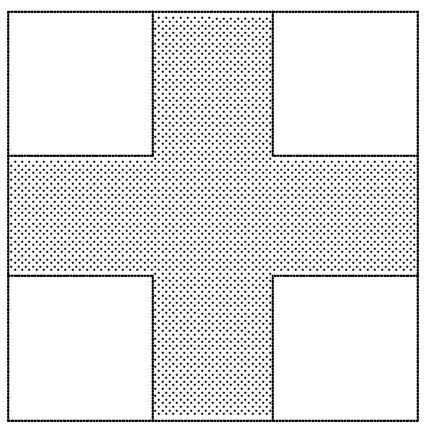
\includegraphics[width=5.5cm]{2te/quadratischefunktion/bilder/kreuz.jpg}
\end{minipage}



\item Die Zinsen eines Kapitals von 800 Euro werden am Ende jeden Jahres zum
Kapital geschlagen und dieses zus"atzlich noch um 100 Euro vermehrt,
so da"s es am Anfang des dritten Jahres auf 1069,28 Euro angewachsen war.
Wie hoch war der ("uber dem gesamten Zeitraum als konstant angenommene) 
Zinssatz?

\item Ein Sch"uler hatte f"ur einen Ferienaufenthalt $252\,$ Euro gespart. Nachdem 
sich die Tageskosten um $7\,$ Euro erh"oht hatten, mu"ste er seinen Aufenthalt 
um drei Tage verk"urzen. Wie viele Tage wollte er urspr"unglich bleiben?


\en 

\ea 

\section{Ungleichungen 2.Grades, Ungleichungssysteme}
Ungleichungen k\"{o}nnen auf dieselbe Art umgeformt werden wie Gleichungen. Ausnahmen
bilden jedoch die Multiplikation (Division) mit einer negativen Zahl und das
Vertauschen. In diesen F\"{a}llen dreht sich das
Ungleichheitszeichen um.\\
In einer \underline{\bf Bruchungleichung} muss daher eine Fallunterscheidung gemacht
werden:\begin{eqnarray}
  \frac{3x+2}{x-4}>2 \quad D=\mathbb{R}\{4\}
\end{eqnarray} \underline{1. Fall:} Unter der Bedingung, dass $x-4>0$ ist, wird die gegebene
Bruchungleichung mit einem positiven Term multipliziert. Das Relationszeichen bleibt
damit erhalten. \begin{eqnarray}
  x>4 \:&\wedge& \: 3x+2>2x-8\\[0.4cm]
  \Leftrightarrow x>4 \:&\wedge& \: x>-10\\[0.4cm]
  L_1&=&\{x|x>4\}
\end{eqnarray} \underline{2. Fall:} Die gegebene Bruchungleichung wird unter der Bedingung, dass
$x-4<0$ ist, mit einem negativen Term multipliziert. Das Relationszeichen wird
umgedreht. \begin{eqnarray}
  x<4 \:&\wedge& \: 3x+2<2x-8\\
  \Leftrightarrow x<4 \:&\wedge& \: x<-10\\
  L_2&=&\{x|x<-10\}
\end{eqnarray} Nun sind beide F\"{a}lle zusammenzufassen. \begin{eqnarray} L=L_1\cup L_2 \Rightarrow L=\{x|x>4  \vee x<-10\}
\end{eqnarray}

\noindent F\"{u}r die L\"{o}sung von \underline{\bf Ungleichungen 2. Grades}
\begin{eqnarray}
ax^2+bx+c>0 \label{groesser}\\
ax^2+bx+c<0 \label{kleiner}
\end{eqnarray}
betrachten wir deren Diskriminante $D$. \\
\underline{1. Fall:} Ist $D>0$ besitzt die Gleichung $ax^2+bx+c=0$ zwei L\"{o}sungen
$x_1,x_2$ wobei wir annehmen, dass $x_1<x_2$. Die Gleichung l\"{a}{\ss}t sich deshalb in
Faktoren zerlegen: $ax^2+bx+c=a(x-x_1)(x-x_2)$. Die Ungleichung \ref{groesser} ist
erf\"{u}llt f\"{u}r alle Werte von $x$ f\"{u}r die gilt $x\not\in (x_1,x_2)$, w\"{a}hrend die
Ungleichung \ref{kleiner}
erf\"{u}llt ist f\"{u}r alle Werte von $x$ f\"{u}r die gilt $x\in (x_1,x_2)$.\\
\underline{2. Fall:} Ist $D=0$ besitzt die Gleichung $ax^2+bx+c=0$ die L\"{o}sung
$x_1=x_2=-\frac{b}{2a}$. Die Gleichung l\"{a}{\ss}t sich in Faktoren zerlegen:
$ax^2+bx+c=a(x-x_1)^2=a(x+\frac{b}{2a})^2$. Die Ungleichung \ref{groesser} ist erf\"{u}llt
f\"{u}r alle Werte von $x$ f\"{u}r die gilt $x\not=-\frac{b}{2a}$, w\"{a}hrend die Ungleichung
\ref{kleiner}
keine L\"{o}sung besitzt.\\
\underline{3. Fall:} Ist $D<0$ besitzt die Gleichung $ax^2+bx+c=0$ keine reelle
L\"{o}sung, das Polynom kann jedoch umgeformt werden:
     \begin{eqnarray}   ax^2+bx+c=a(x^2+\frac{b}{a}x+\frac{c}{a})=\\
       a(x^2+\frac{b}{a}x+\frac{c}{a}+\frac{b^2}{4a^2}-\frac{b^2}{4a^2})=\\
        a[(x^2+\frac{b}{2a})^2-\frac{b^2-4ac}{4a^2}]
     \end{eqnarray}
 Da nun $b^2-4ac$ negativ ist, wird das Polynom f\"{u}r jeden Wert von $x$ positiv.
Die Ungleichung \ref{groesser} ist also f\"{u}r alle Werte von $x$ erf\"{u}llt,
w\"{a}hrend die Ungleichung \ref{kleiner} keine L\"{o}sung besitzt.\\
\underline{\"{U}bungen:}\\
a) lineare Bruchungleichungen: \begin{eqnarray} &1)& \quad \frac{x}{x+1}>0 \qquad \qquad
\quad2)\quad
    \frac{2x}{x+1}\geq 1 \\
&3)& \quad \frac{x-7}{x}<\frac{1-3x}{x} \qquad 4) \quad
    \frac{8-2x}{x+1}\geq1\\
&5)& \quad \frac{x-1}{x}-1<0 \qquad \quad 6)\quad
    \frac{13}{x+4}\leq\frac{15}{2x-3}\\
&7)& \quad \frac{6}{2x-1}>\frac{5}{x-2}\\
&8)& \quad \frac{2}{x-1}\leq\frac{1}{x^2-x}+\frac{1}{x}\\
\end{eqnarray}b) quadratische Ungleichungen: \begin{eqnarray}
\begin{array}{llc@{\qquad}r}
1)& \quad x^2-3x-4 <0   &&[-1<x<4]\\
2)& \quad 2x^2+5x-3 >0  &&[x<-3,x>\frac{1}{2}]\\
3)& \quad x^2-10+25>0   &&[x\in \mathbb{R}\backslash\{5\}\\
4)& \quad 3x^2-5x+9>0   &&[x\in \mathbb{R}]\\
5)& \quad 25-x^2\leq0   &&[x\leq-9; x\geq9]\\
6)& \quad x(3-x)>0  &&[0<x<3]\\
7)& \quad (2x+5)(x-1)<0 &&[-\frac{5}{2}<x<1]\\
8)& \quad (x-1)(x+2)>0  &&[x<-2;x>1]\\
9)& \quad x(x-3)+\D{\frac{x}{2}}>(2x-5)^2+\D{\frac{7x^2}{3}}    &&\\[0.4cm]
10)& \quad 5x^2-11<(2x-1)^2-\D{\frac{x^2-1}{4}}+11      &&\\[0.4cm]
11)& \quad (3x-2)^2+3<5x-(2x-1)^2   &&[\frac{8}{13}<x<1]\\[0.4cm]
12)& \quad \D{\frac{x^2+4x}{6}}>\D{\frac{9x+36}{2}}-35 &&[x<6;x>17]\\[0.4cm]
13)& \quad 2(x-1)-(x+3)^2+4x-6<0    &&[x\in \mathbb{R}]\\[0.4cm]
14)& \quad \D{\frac{x-1}{5}+\frac{1}{3}}<\D{\frac{x^2-5x+6}{6}}
            &&[x<1,x>\frac{26}{5}]\\[0.4cm]
15)& \quad \D{\frac{(x+3)^2}{5}-\frac{7(x-6)}{2}}\leq\D{\frac{(2x-20)
    (x-12)}{3}}-\frac{x}{2}     &&[x\leq\frac{39}{7},x\geq22]\\[0.4cm]
15)& \quad \D{\frac{x+3}{x}}>\D{\frac{x}{x+3}}
\end{array}
\end{eqnarray}

\underline{Ungleichungssysteme:}\\
Bei Ungleichungsystemen l\"{o}st man die gegebenen Ungleichungen und bildet dann die
Schnittmenge der einzelnen L\"{o}sungen.
%\input{funktion_quadrat}


\section{Der Scheitel der Parabel}

Jede Parabel hat einen gr��ten bzw. kleinen Wert, diesen nennt man {\bf Scheitel}. 

\bs  Eine quadratische Funktion $y=ax^2+bx+c$ hat immer einen Scheitelpunkt $S(x_s, y_s)$ mit $$x_s=-\frac{b}{2a}$$ Die Parabel ist immer symmetrisch bez�glich der Geraden durch den Scheitel, also bez�glich $x=x_s$.\es 

\begin{proof}
Die Formel kann auf zwei Arten bewiesen werden: \bn \item Mit Hilfe der quadratischen Erg�nzung. \item Das arithmetische Mittel der Nullstellen ...  \en 
\end{proof}






\ba \bn \item 
Gegeben ist die Funktion $f: y=x^2+x-3,75$.
\begin{enumerate}
\item
Bestimme die maximale Definitions- und Wertemenge der Funktion.
\item
Gib die Koordinaten des Scheitelpunktes $S(s_1|s_2)$ an.
\item
Zeichne den Graphen der Funktion im Intervall $[s_1 -3;s_1 +3]$.\\
(1 L"angeneinheit = $1 \, \rm cm$)
\item
Bestimme \underline{rechnerisch} die Nullstellen der Funktion $f$.
\end{enumerate}

\item
Gegeben ist die Funktion $f(x) = -1,5x^2 + 9x - 12$.\\
Bestimme die Koordinaten des Scheitels sowie die Bereiche auf der 
$x$-Achse, in denen die Funktion steigt bzw. f"allt.

\item
 
Gegeben ist die Funktion $p: y= -0,5x^2 + x + 1,5$.
\begin{enumerate}
\item
Zeige, da"s der Punkt $S(1|2)$ Scheitel der zu p geh"orenden Parabel ist.
\item
Bestimme die Symmetrieachse, Wertemenge und die Schnittpunkte des Graphen
mit den Koordinatenachsen.
\item
Zeichne den Graphen der Funktion im Intervall $[-3;5]$ ohne Verwendung
einer Wertetabelle. (1 L"angeneinheit = $1 \, \rm cm$)
\end{enumerate}

\item
 
Bestimme die Scheitelpunktsform folgender Funktionen und gib jeweils
die Koordinaten des Scheitels an:
\begin{enumerate}
\item
$ x \mapsto 3 x^2 - 6x - 3$
\item
$ x \mapsto 2x^2 + 4x - 3$
\end{enumerate}
\en
\ea 

\ba Computerraum
\begin{enumerate}
\item Besuche die Seite
http://www.mathe-online.at/galerie/fun1/fun1.html
und f�hre die folgenden 3 Java-Applets aus - bitte konzentriert arbeiten!
	a.) Funktionen erkennen 1 	
	b.) Graphen erkennen 1
      c.) Graphen zeichnen

\item Puzzlespiele:

\bn \item \url{http://johnny.ch/math/puzzle/lin_funkt_.php}

\item  \url{http://johnny.ch/math/puzzle/quad_funkt2.php}

\item \url{http://www.mathe-online.at/tests/fun1/erkennen.html}
\en 

\item Besuche die Seite 
	\url{http://de.wikipedia.org/wiki/Quadratische_Funktion}
und lies die Abschnitte 1.1 bis 1.5 konzentriert durch - was ist neu? Notiere dir das Wesentliche!

\item Der Mathemillion�r: \url{http://www.thorsten-vogelsang.de}

\item �bung Computerraum:

�ffne die Seite \begin{verbatim}
http://www.cybernautenshop.de/virtuelle_schule/lehrinhalte_index2.html
\end{verbatim}
und gehe zu den abgebildeten Kapiteln. Gute Arbeit!

\begin{center}
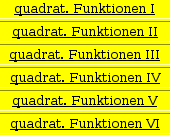
\includegraphics[width=3cm]{2te/quadratischefunktion/bilder/quadratischefunktionen.png}
\end{center}


\end{enumerate}
\ea 




\section{Schnittpunkte von Funktionen}

Sucht man die Schnittpunkte von zwei Funkionsgraphen $f_1$ und $f_2$, so muss man 
\bi \item die Funktionen gleichsetzen $f_1(x)=f_2(x)$
    \item die Gleichung l�sen.
\ei 

Schneidet man nun eine quadratische Funktion mit einer linearen, oder mit einer weiteren quadratischen, so entsteht immer eine quadratische Gleichung, welche keine, eine oder zwei L�sungen haben kann. Entsprechend gibt es keinen Schnittpunkt, einen sog. {\it Ber�hrungspunkt} oder zwei Schnittpunkte.

\begin{center}
\begin{tabular}{|p{4.5cm}p{4.5cm}p{4.5cm}|} \hline 
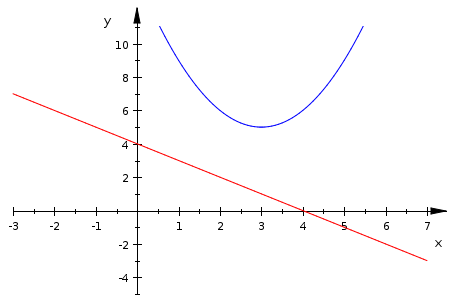
\includegraphics[width=4.5cm]{2te/quadratischefunktion/bilder/schnittparabel04.png}  & 
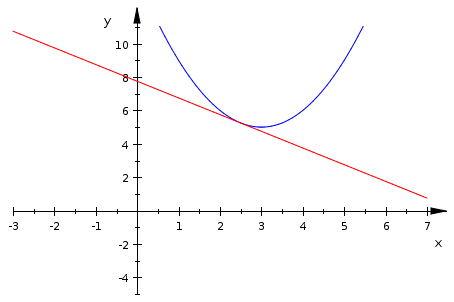
\includegraphics[width=4.5cm]{2te/quadratischefunktion/bilder/schnittparabel05.png}  & 
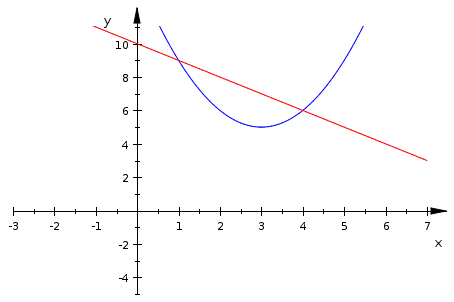
\includegraphics[width=4.5cm]{2te/quadratischefunktion/bilder/schnittparabel06.png}  \\
kein Schnittpunkt, Gerade ist eine {\it Passante} & ein Ber�hrungspunkt, Gerade ist eine {\it Tangente} & zwei Schnittpunkte, Gerade ist eine {\it Sekante} \\
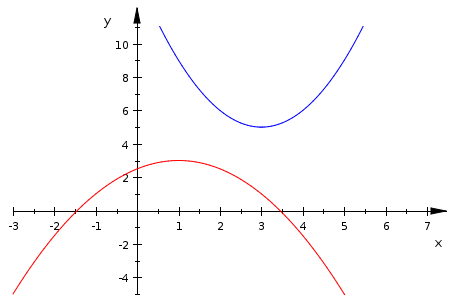
\includegraphics[width=4.5cm]{2te/quadratischefunktion/bilder/schnittparabel01.png}  & 
\includegraphics[width=4.5cm]{2te/quadratischefunktion/bilder/schnittparabel02.png}  & 
\includegraphics[width=4.5cm]{2te/quadratischefunktion/bilder/schnittparabel03.png}  \\ \hline 
\end{tabular}
\end{center}

\bb Grundaufgaben
\bn \item Berechne die Schnittpunkte einer Geraden mit einer Parabel.
\item Berechne die Schnittpunkte zweier Parabeln.
\item Berechne einen Parameter, so dass es keine, bzw. genau einen, bzw. zwei Schnittpunkte gibt.
\en  
\eb


\ba \bn \item 
Gegeben ist die quadratische Funktion

$ y=-\frac{2}{3}\,x^2-3x+\frac{13}{8}$ ~~mit der Definitionsmenge $D=[-6;0]$.
\begin{enumerate}
\item   Zeichne den Graphen nach Berechnung der Scheitelkoordinaten sowie
        der Randpunkte sauber in ein Koordinatensystem ein!
\item   Gib die Wertemenge $\mathbb{W}$ an!
\item   Die Gerade mit der Gleichung $y=\frac{7}{3}$ schneidet den 
        Funktionsgraphen in zwei verschiedenen Punkten $P$ und $Q$.\\
        Trage $P$ und $Q$ in die Zeichnung ein und \underline{berechne}
        die Koordinaten dieser Punkte!
\end{enumerate}


\item
 Gegeben sind die Parabeln $p_1: \; y=0,5x^2+x+1,5$ und $p_2: \; y=-x^2+4x$\\
Untersuche \underline{rechnerisch}, ob sich die Parabeln schneiden.\\
Gib gegebenenfalls die Koordinaten gemeinsamer Punkte an.


\item Gegeben ist die Funktion $y=-1/2x^2+4x-5$ und die Geradenschar $y=kx+3$. F�r welche Werte von $k$ ist die Gerade Tangente an die Parabel?
\en

\ea 


\section{Die quadratische Interpolation}


\begin{minipage}{10cm}Sind zwei Punkte gegeben und eine Gerade (also eine lineare Funktion $y=kx+d$) gesucht, so f�hrt die Aufgabe auf ein lineares Gleichungssystem mit zwei Unbekannten (vgl. Kapitel \ref{linfkl_lings} auf Seite \pageref{linfkl_lings}). - Man nent diese Aufgabe auch {\bf lineare Interpolation}.

Bei einer {\bf quadratischen Interpolation} sucht man nun eine quadratische Funktion, also Werte f�r $a,b$ und $c$, so dass der Graph durch 3 gegebene Punkte verl�uft. Die Vorgehensweise ist dabei wieder dieselbe: Man muss dabei die drei Punkte in diese Gleichung einsetzen und  ein lineares Gleichungssystem mit drei Gleichungen und drei Unbekannten l�sen.

Welche Funktion verl�uft durch die  gezeichneten Punkte rechts?\\
		..............      
		\end{minipage} 
		\begin{minipage}{4cm}
		\includegraphics[width=4cm]{2te/quadratischefunktion/bilder/quadinterpol.jpg}
		\end{minipage}

\ba 
\bn \item Bestimme ausf"uhrlich die Gleichung derjenigen Parabel, welche durch
         die Punkte $P(-1|2),~Q(3|-22),~R(-7|-7)$ verl"auft!


\item Von einer Parabel ist der Scheitel $S(2|3)$ gegeben sowie der Punkt $(7|-1)$ Wie lautet die Funktionsgleichung?

\item
Der Graph der Funktion $x \mapsto ax^2 + bx + c$ ber"uhrt die x-Achse 
im Punkt $P(7|0)$ und geht durch den Punkt $Q(2|-75)$.\\
Bestimme a, b und c und gib diese Funktion an!

\item 
 
Der Graph einer Funktion $y=ax^2 + bx + c$ hat den Scheitel $S(10|-1)$
und geht durch den Punkt $P(9|2)$.
Bestimme a, b und c.
\en 
\ea 



\section{Extremwertaufgaben mit Parabeln}
Mit Extremwertaufgaben besch�ftigen wir uns eigentlich erst in der 5. Klasse (Differentialrechnung). Es geht im Allgemeinen darum, einen kleinsten oder gr��ten Funktionswert (in einem bestimmten Bereich) zu finden. Bei Parablen f�hrt diese Aufgabe auf die Berechnung des Scheitels. Dabei ist die $x$-Koordinate des Scheitels die {\it Extremstelle} und die $y$-Koordinate des Scheitels der {\bf Extremwert}.


\ba 
\bn 
\item 
Hat die Funktion $y = -0,8 x^2 + 0,2 x + 4$ einen gr"o"sten oder 
kleinsten Funktionswert? Begr"undung! Bestimme diesen Wert und gib
an, f"ur welchen x-Wert sie ihn annimmt. In welchem Bereich
(der x-Werte) steigt, in welchem f"allt der Graph der Funktion?

\item
 
Bilde ein Produkt, dessen erster Faktor um 1 gr"o"ser als $x$ und dessen
zweiter Faktor um 3 kleiner als $x$ ist. F"ur welche Zahl $x$
ist der Wert dieses Produkts am kleinsten?


\item
 
\begin{center}
\includegraphics[width=4cm]{2te/quadratischefunktion/bilder/kanone.jpg}
\end{center}

Die Flugbahn einer Kanonenkugel ist eine Parabel. Der Scheitel der
Flugbahn hat die Koordinaten S$(\,400\,{\rm m}\,|\,675\,{\rm m}\,)$,
der Abschusspunkt liegt in einer Felswand bei 
A$(\,200\,{\rm m}\,|\,375\,{\rm m}\,)$.
\begin{enumerate}
\item Berechne die Gleichung der Flugbahn in der Form $y=a\,x^2+b\,x+c$.
\item Bei welcher $x$-Koordinate f"allt die Kugel ins Meer?
\item \parfillskip0pt Die Flugbahn wird parallel zur $y$-Achse soweit
  nach oben verschoben, bis der Auftreffpunkt im Meer  
\end{enumerate}

\begin{enumerate}
\item[] bei $x=800\,$m liegt. 

Berechne die H"ohe $h'$ des neuen Abschusspunktes A$'(\,200\,{\rm m}\,|\,h'\,)$.
\item[(d)] Zeichne die beiden Flugbahnen in {\bf ein} Koordinatensystem 
($1\,{\rm cm}\,\widehat{=}\,100\,$m).
\end{enumerate}

\item
 
Zeige: Von allen Rechtecken mit Umfang $8\,\rm cm$ hat das Quadrat mit
Seitenl"ange $2\,\rm cm$ den gr"o"sten Fl"acheninhalt.


\item

 \begin{minipage}[t]{8cm}
Ein Quadrat ABCD hat die Seitenl"ange $4\,$cm. Tr"agt man von der Ecke C auf 
beiden anliegenden Seiten jeweils x cm ab, so erh"alt man die Punkte P 
und Q.\\
F"ur welchen x-Wert hat das Dreieck APQ den gr"o"sten Fl"acheninhalt?\\
Wie gro"s ist dieser?
\end{minipage}
\begin{minipage}[t]{6cm}
\includegraphics[width=6cm]{2te/quadratischefunktion/bilder/quadrat2.jpg}\end{minipage}


\en 

\ea 
 \chapter{Die beschreibende Statistik}





 {\it Stochastik} kommt aus dem Griechischen und bedeutet soviel wie "`Kunst des Mutma{\ss}ens"'.
 Heute teilt man die Stochastik in
 {\bf Statistik} und {\bf Wahrscheinlichkeitsrechnung} ein.


In der Statistik will man Aussagen �ber eine Grundgesamtheit machen; da selten die gesamte Grundgesamtheit befragt, untersucht, beobachtet, ... werden kann muss man sich auf eine Auswahl, einer Stichprobe beschr�nken. Diese
Stichprobe gibt zwar eine gewisse, aber keine vollst\"{a}ndige und sichere Auskunft \"{u}ber die
Grundgesamtheit. Voraussagen bzw. Entscheidungen m\"{u}ssen sich jedoch stets an der
Grundgesamtheit orientieren. Ein wesentliches Problem der Statistik besteht also darin, von einer
Stichprobe auf die Grundgesamtheit zu schlie{\ss}en. Mit diesem Problem besch\"{a}ftigt sich die
{\bf Beurteilende Statistik}; sie benutzt dabei als entscheidendes Hilfsmittel die {\bf
Wahrscheinlichkeitsrechnung}. Bei der beurteilenden Statistik werden also Stichproben untersucht
und Schl\"{u}sse auf die Grundgesamtheit gezogen. Im Unterschied zur Beurteilenden Statistik
f\"{a}llt das Planen und Durchf\"{u}hren statistischer Erhebungen sowie die zweckm\"{a}{\ss}ige
Aufbereitung der dabei gewonnenen Daten in das Gebiet der {\bf Beschreibenden Statistik}. Daten werden also erfasst und anschlie�end durch {\it Tabellen} (vgl. Kapitel \ref{hfkdsm} ab Seite \pageref{hfkdsm}), {\it Graphiken} (Kapitel \ref{grphkeit} ab Seite \pageref{grphkeit}) und {\it Kennzahlen} (Kapitel \ref{statmasz} ab Seite \pageref{statmasz}) �bersichtlich beschrieben.

  \begin{figure}[htb]
  \begin{center}
    \includegraphics[width=10cm]{2te/beschreibendestatistik/bilder/stochast.jpg}
  \caption{Einteilung der Stochastik}
  \end{center}
  \end{figure}



Die Wahrscheinlichkeitsrechnung entstand im 17.
Jahrhundert aus dem Bestreben, bei Gl\"{u}cksspielen Gesetzm\"{a}{\ss}igkeiten f\"{u}r {\it
Zufallsereignisse} zu finden und so Gewinn bringende Spieltechniken zu entwickeln; es sollten damit
g\"{u}nstige Ausg\"{a}nge eines Zufallsexperimentes vorhergesagt werden.

\ba \label{auf_augensumme} Es wird mit zwei W\"{u}rfeln geworfen und die Augensumme addiert. Auf
welche Augensumme sollte man setzen?\ea



\begin{minipage}{10cm}Die Mathematiker {\it Fermat} und {\it
Pascal} behandelten
zun\"{a}chst Einzelprobleme, erst {\it Bernoulli} und {\it Laplace} erreichten im 18. und 19. Jahrhundert eine weitgehende
Systematisierung. Im Vergleich zur anderen Teilgebieten der Mathematik, wie etwa Geometrie, handelt
es sich also hier um eine relativ junge Wissenschaft.

Piere de Fermat, 1601-1665, franz. Mathematiker\\Blaise Pascal, 1623-1662, franz. Philosoph und Mathematiker\\Jakob Bernoulli, 1655-1705, schweizer
Mathematiker\\Simon de Laplace, 1749-1827, franz\"{o}sischer
Mathematiker und Astronom
\end{minipage}
\begin{minipage}{5cm}
%\begin{figure}
%\centering
\includegraphics[height=4.5cm]{2te/beschreibendestatistik/bilder/mathe_stoch.jpg}

Fermat - Pascal - Laplace - Bernoulli (von l.o. nach r.u.)
\end{minipage}

\subsection*{Ausblick}
Wir werden uns m�glichst jedes Jahr einen Teil vornehmen, geplant ist folgende Aufteilung:
\begin{description}
\item [Beschreibende Statistik] 2. Klasse
\item [Kombinatorik und zweidimensionale Statistik] 3. Klasse
\item [Wahrscheinlichkeitsrechnung] 4. Klasse
\item [Wahrscheinlichkeitsverteilungen und beurteilende Statistik] 5. Klasse
\end{description}



\section{Allgemeines zur beschreibenden Statistik}


\ba \label{auf_meran} In Meran finden Gemeinderatswahlen statt. Dabei gewinnt die Partei "`LPM"'
des Spitzenkandidaten Korruptikus mit $28\%$ der Stimmen. An Korruptikus selbst  gehen $51\%$ der
Stimmen. Am n\"{a}chsten Tag steht in der parteiabh\"{a}ngigen (!) Tageszeitung: "`Korruptikus hat
die absolute Mehrheit von $51\%$ - Danke!"'.

Was ist von dieser Aussage zu halten, wenn in Meran $26.000$  B\"{u}rger wahlberechtigt sind und
die Wahlbeteiligung bei $70\%$ lag? \ea

Vielleicht kennt jemand das gefl\"{u}gelte Wort:

\begin{quotation}"`Trau keiner Statistik, die du nicht selber gef\"{a}lscht hast!"'. \end{quotation}



 Die damit formulierte Skepsis gegen\"{u}ber der Statistik h\"{a}ngt vermutlich mit der {\bf typischen Arbeitsweise dieser
 Wissenschaft} zusammen: Wenn Politiker, Beh\"{o}rden oder Manager wissen m\"{o}chten, wieviel die Arbeitnehmer verdienen, wie viele Kinder
die Familien haben, wie lange die Studenten studieren, welche Waschmittel die Haushalte bevorzugen
usw., so ist es in der Regel unm\"{o}glich oder zu kostspielig, die ganze sie interessierende {\it
Grundgesamtheit} zu befragen (sog. {\it Vollerhebung}), sondern man ist angewiesen auf die Aussagen
einer (gen\"{u}gend gro{\ss}en) Auswahl (sog. {\it Stichprobe}). Ohne statistische Erhebungen
\"{u}ber Verkehrsaufkommen, Wirtschaftsentwicklungen, Sch\"{u}lerzahlen usw. ist heute eine
notwendige Planung f\"{u}r die n\"{a}here oder fernere Zukunft nicht mehr denkbar.

\subsubsection{Wie man mit Statistik l\"{u}gt}
Missbr\"{a}uche der Statistik sind so zahlreich, dass es sogar ganze B\"{u}cher dar\"{u}ber gibt.
Ihre Ursachen reichen von Dummheit und Naivit\"{a}t \"{u}ber zwielichtiges geschicktes
Man\"{o}vrieren "`an den Grenzen der Legalit\"{a}t"' bis hin zu glattem Betrug. Man denke nur an
Werbung und Politik; aber selbst in der Wissenschaft muss man auf der Hut sein. Zu den Quellen, die
die sprichw\"{o}rtliche "`Verdrehbarkeit"' der Statistik erm\"{o}glichen, geh\"{o}ren die
folgenden:

\bn \item Unkenntnis der statistischen Methoden und ihrer vern\"{u}nftigen Anwendung.

\item Zahlen sind nicht immer exakt. Im Gegensatz zu Zahlen in der Reinen Mathematik ist
eine Zahl in der Angewandten Statistik stets etwas Verschwommenes, mit einem zuf\"{a}lligen Fehler
behaftet; und wenn die Gr\"{o}{\ss}enordung dieses Fehlers (z.B. durch Angabe eines
"`Standardfehlers"' oder Angabe der geltenden Ziffern) nicht klar aus dem Kontext hervorgeht, so
ist die Zahl wertlos, da sie alles bedeuten kann.



\item Viele Zahlen und Diagramme bedeuten bei genauem Hinsehen etwas ganz anderes, als suggeriert wird; oder es
l\"{a}sst sich \"{u}berhaupt nicht eruieren, was sie eigentlich bedeuten (Reklame, Politik,
Polemiken, ...).  \ba Finde selbst ein Beispiel zu dieser Aussage!\ea


\item Oft wird wichtige Zusatzinformation (versehentlich oder absichtlich) unterschlagen.




\item  Es ist oft erstaunlich schwer zu beurteilen, auf welche Populationen sich ein Ergebnis verallgemeinern
l\"{a}sst. Das gilt insbesondere auch f\"{u}r zeitliche Extrapolation (Prognosen, z.B. Wirtschafts-
oder Bev\"{o}lkerungsprognosen). \en


Einige Standardfragen an zweifelhafte Statistiken sind:

\bi \item Na und, was soll's?

\item Was f\"{u}r eine Absicht steckt dahinter?

\item Was fehlt? Was wurde vergessen oder verschwiegen?

\item Woher wei{\ss} man das?

\item Was besagt das wirklich?
\ei

Also, es ist Vorsicht geboten!

 Im Idealfall erstreckt sich eine statistische Erhebung auf s\"{a}mtliche Individuen
(Merkmalstr\"{a}ger) der Grundgesamtheit. Jedes Individuum wird hierbei auf ein bestimmtes Merkmal
untersucht. Oft ist es z.B. aus Zeit- oder Kostengr\"{u}nden jedoch nicht m\"{o}glich, manchmal zur
Erlangung der gew\"{u}nschten Information auch gar nicht n\"{o}tig, alle Individuen der
Grundgesamtheit zu befragen. Man begn\"{u}gt sich mit einer Auswahl, einer sog. Stichprobe.
Allgemein bekannt ist dieses Vorgehen bei Meinungsumfrage; eine zuf\"{a}llig ausgew\"{a}hlte Anzahl
von Personen wird dabei nach ihrer Meinung befragt.



\subsection{Erhebung von Daten}

F\"{u}r viele Fragestellungen kann man auf Daten zur\"{u}ckgreifen, die bereits f\"{u}r andere
Untersuchungen erhoben und in statistischen Jahrb\"{u}chern, amtlichen Statistiken usw.
Festgehalten sind. Man spricht in diesem Fall von {\it sekund\"{a}rstatistischen} Erhebungen.

Stehen aber f\"{u}r die eigene Untersuchung solche Daten nicht zur Verf\"{u}gung, m\"{u}ssen sie in
einer {\it prim\"{a}rstatistischen} Erhebung selbst erhoben werden.

Einige Probleme bei der Datenerhebung:

\bi \item Probleme entstehen bei der Auswahl der Befragten, der Formulierung der Fragen, beim
Aufbau des Fragebogens usw.

\item Die Frage nach dem Geschlecht erscheint unproblematisch, bei der Frage nach dem Alter kann es bereits
Schwierigkeiten geben. Auch ist es nicht jedermanns Sache, bekanntzugeben, dass man t\"{a}glich
sechs Stunden vor dem Fernsehapparat sitzt, h\"{a}ufiger die Werbung als die Nachrichten und man am
liebsten Kindersendungen sieht.

\item Bei einer geringen Zahl an Befragten ist die Anonymit\"{a}t nicht gew\"{a}hrleistet. Aus den Angaben \"{u}ber Alter
und Geschlecht wird man oft auf eine bestimmte Person schlie{\ss}en k\"{o}nnen. \ei

 Statistische Aussagen sind
bestenfalls so gut wie die Daten, auf die sie sich beziehen.


\subsubsection*{Es stimmt nicht, dass ...}
\bi \item ... man mit Statistik alles beweisen kann. (In einem engeren Sinn kann man sogar
behaupten, dass sich Hypothesen nur statistisch widerlegen, niemals aber beweisen lassen.)
Allerdings l\"{a}sst sich bekanntlich Statistik leicht und stark zu ,,L\"{u}gen`` verschiedenster
Art missbrauchen.


\item ... die Befragung von 1000 Menschen aus einer Million genauso dumm und nichts sagend ist wie die von einem
Menschen aus 1000. Sie ist etwa so informativ wie die Befragung von 500 aus 1000, oder von 1001 aus
einer unendlichen Grundgesamtheit.

\item ... jemand mit den F\"{u}{\ss}en im Eis und dem Kopf im Feuer sich im statistischen Mittel wohl f\"{u}hlt. Die Streuung
ist meist genauso wichtig wie das Mittel (vgl. \label{statmasz} ab Seite \label{statmasz}).\ei

\subsection{Wozu Statistik lernen?}


Grundkenntnisse der Statistik erm\"{o}glichen es ...

\bi \item ... kleine statistische Anwendungsprobleme mit den eigenen Daten (angefangen bei der
Facharbeit selber zu l\"{o}sen; ...)

\item bei gr\"{o}{\ss}eren Problemen sinnvoll mit dem beratenden Statistiker zusammenzuarbeiten;

\item ... die Statistik in anderen wissenschaftlichen Arbeiten oder auch nur in Zeitschriften
(wenigstens in den Grundz\"{u}gen) zu verstehen;

\item ... die vielen Missbr\"{a}uche und Fehler leichter zu durchschauen und selbst\"{a}ndig zu beurteilen.
\ei

Die Statistik trainiert das Abstraktionsverm\"{o}gen, erweitert die Allgemeinbildung und bereitet
dem einen oder anderen sogar Freude \"{u}ber neue F\"{a}higkeiten und Erkenntnisse.



\subsection*{Buchempfehlungen aus der Bibliothek}
In userer Bibliothek findest du zahlreiche interessante, unterhaltsame und gleichzeitig aber auch lehrreiche Lekt�re zu diesem Thema - wer zuerst kommt malt bekanntlich zuerst ...
\begin{itemize}
\item [$\rhd$] {\it Denkste, Popul�re Irrtumer, beliebte Denkfehler, moderne Zahlenmythen} Walter Kr�mer
\item [$\rhd$]{\it So l�gt man mit Statistik} Walter Kr�mer  	
\item [$\rhd$]{\it Das Einmaleins der Skepsis} 	Gigerenzer
\item [$\rhd$]{\it Mit an Wahrscheinlichkeit grenzender Sicherheit - Logisches Denken und Zufall} Dubben, Hans-Hermann - Beck-Bornholdt, Hans-Peter 
\item [$\rhd$]{\it Der Hund, der Eier legt Erkennen von Fehlinformation durch Querdenken } 	Hans-Peter; Dubben, Hans-Hermann
\item [$\rhd$]{\it Der Schein der Weisen. Irrt�mer und Fehlurteile im t�glichen Denken.} Hans-Peter Beck-Bornholdt, Hans-Hermann Dubben
\item [$\rhd$]{\it  Die Welt als Roulette Denken in Erwartungen} Basieux, Pierre 	
\item [$\rhd$]{\it Es war 1 mal . . . Die verborgene mathematische Logik des Allt�glichen} Paulos, John A.
\item [$\rhd$]{\it Das Universum in der Teetasse Von der allt�glichen Magie der Mathematik} Cole, K. C. 
\item [$\rhd$] {\it Das Ziegenproblem Denken in Wahrscheinlichkeiten}  Gero von Randow
\end{itemize}




\section{Grundbegriffe}
\subsection{Merkmale und Merkmalsauspr\"{a}gungen} Bei einer statistischen Erhebung wird an
den {\it Merkmalstr\"{a}gern} (Individuen) das interessierende {\it Merkmal} in bestimmten {\it
Merkmalsauspr\"{a}gungen} beobachtet. Durch die Erhebung soll festgestellt werden, wie die
verschiedenen Auspr\"{a}gungen des Merkmals in der Grundgesamtheit der Merkmalstr\"{a}ger verteilt
sind.



\bd  Die einer statistischen Erhebung zugrundeliegende
{\it Menge von Merkmalsauspr\"{a}gungen} wird mit {\bf S}, ihre $k$ Elemente werden mit $a_1, \dots,
a_k$ bezeichnet. Es ist also: $S=\{a_1, a_2, \dots, a_k\}$. \ed



\subsection{Arten von Merkmalen}
Man unterscheidet nun zwischen {\bf qualitativen}, - und {\bf quantitativen}
Merkmalsauspr\"{a}gungen.


 \begin{figure}[htb]
  \begin{center}
    \includegraphics[width=10cm]{2te/beschreibendestatistik/bilder/merkmal1.jpg}
  \caption{\"{U}bersicht \"{u}ber die Merkmalsarten}
  \end{center}
  \end{figure}  

\begin{itemize}
  \item Die {\bf qualitativen Merkmale} sind die Merkmalsauspr\"{a}gungen nur
  {\it Beschreibungen}, sind also nicht messbar. Qualitative Merkmale erlauben keinen direkten Gr\"{o}{\ss}envergleich;
  sie erlauben nur einen Vergleich der Art
  gleich oder ungleich (z.B. Beruf,
Religionszugeh\"{o}rigkeit, Farbe, $\dots$).
  \item {\bf Quantitative}  Merkmale
  sind immer angeordnet und die Abst\"{a}nde zwischen den
  Merkmalsauspr\"{a}gungen sind mathematisch interpretierbar.
   Eine Auspr\"{a}gung nennt man 
quantitativ, wenn sie nur {\it durch Zahlen darstellbar} ist (z.B. K\"{o}rpergr\"{o}{\ss}e, Taillenweite, Einwohnerzahl, Monatseinkommen, Fettgehalt von
Milch, $\dots$). Quantitative Merkmale werden noch
eingeteilt in
   \begin{itemize}
      \item {\bf stetige} Merkmalsauspr\"{a}gungen, wenn sie jeden beliebigen Wert (also auch jede Dezimalzahl) in einem bestimmten
        Intervall aus $\mathbb{R}$ annehmen k\"{o}nnen, die K�rpergr\"{o}{\ss}, das K�rpergericht, das Einkommen sind Beispiele f�r stetige Daten.

      \item {\bf diskrete} Merkmalsauspr\"{a}gungen, wenn nur
    bestimmte Werte m\"{o}glich sind. So ist die Anzahl der Kinder in
    einer Familie ein Beispiel f\"{u}r diskrete Daten.
    \end{itemize}
Im Allgemeinen gilt, dass Messungen zu stetigen Daten, Aufz\"{a}hlungen hingegen zu diskreten Daten
f\"{u}hren.
\end{itemize}



\ba \bn \item Erg�nze:

\begin{tabular}{|l|l|l|}
  % after \\: \hline or \cline{col1-col2} \cline{col3-col4} ...
 \hline  Merkmalstr\"{a}ger & Merkmal & Merkmalsauspr\"{a}gungen \\ \hline
  Personen & Familienstand & $\dots$ \\
   & Geburtsmonat &  $\dots$\\
   & K\"{o}rpergr\"{o}{\ss}e & $\dots$ \\
  Versuchstiere & Schmerzreaktion & ja, ... \\
  Fertigprodukte & Qualit\"{a}t & 1. Qual, 2. Qual., Ausschuss \\
  W\"{u}rfelw\"{u}rfe & Augenzahl & $\dots$ \\
  M\"{u}nzw\"{u}rfe & Seite & $\dots$ \\ \hline
\end{tabular}



\item Die Abbildung  ist aus der Tageszeitung Dolomiten entnommen. Versuche die folgenden Aufgaben zu
l\"{o}sen: 

\begin{minipage}{8cm}
\bn
\item Bestimme, ob sich um eine Stichprobe handelt und gib gegebenenfalls den Stichprobenumfang an.
\item Bestimme den Merkmalstr\"{a}ger, das Merkmal, die Merkmalsauspr\"{a}gungen und die Art des Merkmals!
\item Diese Grafik enth\"{a}lt einen wesentlichen Fehler! Welchen?
\en
\end{minipage}
\begin{minipage}{7cm}
    \includegraphics[width=6.5cm]{2te/beschreibendestatistik/bilder/freizeit.jpg}\\
\end{minipage}


\item \label{auf_bienen} 
 Gib die Anzahl $k$ und die Menge von Merkmalsauspr\"{a}gungen an bei einer Befragung nach:
   

 der Staatsangeh\"{o}rigkeit, der Anzahl leiblichen Kinder, der Schulbildung,  dem K\"{o}rpergewicht.
   

\item Ein Bienenz\"{u}chter untersucht, ob seine Bienen von der Milbenkrankheit befallen sind. Welche Menge von
Merkmalsauspr\"{a}gungen legt er zugrunde?
\item Merkmalstr\"{a}ger seien Wohnh\"{a}user. Gib verschiedene Merkmale an, die man an diesen Merkmalstr\"{a}gern untersuchen
kann.
 


\item  Werden die Fehlstunden im ersten Semester  aller Sch\"{u}ler der 5. Klassen einer Schule
untersucht, so sind die Merkmalstr\"{a}ger ...., das Merkmal ....., die Merkmalsauspr\"{a}gung ....

\item  \label{auf_puls} Gib bei der folgenden Tabelle an, welche Art der
Merkmalsauspr\"{a}gung vorliegt, bei quantitativen Merkmalen ist weiters anzugeben, ob es sich um
diskrete oder stetige Merkmale handelt.


\begin{tabular}{|l|l|l|p{2.5cm}|}\hline
Merkmalstr\"{a}ger        &Merkmal &Merkmalsauspr\"{a}gungen & Art\\\hline
    a)Sch\"{u}ler im Wisslyz   &K\"{o}rpergr\"{o}{\ss}e & &\\ 
    b)Sch\"{u}ler im Wisslyz S   &Geschlecht & &\\ 
    c)Sch\"{u}ler im Wisslyz S   &K\"{o}rpergewicht & &\\ 
    d)Angestellte beim Land &Familienstand & & \\  \hline
\end{tabular}



  \item Welche der folgenden Merkmale sind qualitativ, welche quantitativ?
 Gr\"{o}{\ss}e eines Bauplatzes; Schultyp; Staatsangeh\"{o}rigkeit; Dicke eines Leitungsdrahtes; Geschwindigkeit; Gangart bei einem PKW
    
  \item Pr\"{u}fe, ob die folgenden quantitativen Merkmale diskret oder stetig sind: 
   Pulsschl\"{a}ge je Minute;   Benzinverbrauch je 100 km; Zigarettenverbrauch je Tag;  Lautst\"{a}rke. \en \ea



\section{H\"{a}ufigkeiten und ihre Darstellungsm\"{o}glichkeiten}\label{hfkdsm}
\subsection{Ur- und Strichlisten} 


Bei der Durchf\"{u}hrung einer statistischen Erhebung (Stichprobe) werden zun\"{a}chst alle
Ergebnisse (Daten) in einer sogenannten {\bf Urliste} notiert oder als Urliste gesammelt, bevor sie
weiter aufbereitet werden. Dabei hei{\ss}en die einzelnen Beobachtungswerte der Urliste {\bf
Stichprobenwerte} (oder: Daten) und werden mit $x_1, x_2, \dots, x_n$ bezeichnet. (Warum genau
$n$?)


Um einen schnellen \"{U}berblick \"{u}ber die Stichprobenwerte zu erhalten, verwendet man
h\"{a}ufig {\bf Strichlisten}. Dabei wird jeder Stichprobenwert $x_i$ genau einer
Merkmalsauspr\"{a}gung $a_j$ zugeordnet. Strichlisten sind schon viel \"{u}bersichtlicher als eine Urliste.

\ba \bn \item  \label{bbabc} Anl\"{a}sslich einer "`Schulstatistik"'  wurde in einer Klasse das
Alter der Sch\"{u}ler festgestellt. Von den 20 Sch\"{u}lern wurden folgende Zahlen genannt:
\begin{center}
\begin{tabular}{cccccccccc}
  % after \\: \hline or \cline{col1-col2} \cline{col3-col4} ...
  18 & 19 & 17 & 18 & 18 & 17 & 19 & 18 & 18 & 21 \\
  18 & 19 & 19 & 18 & 17 & 19 & 18 & 18 & 19 & 18 \\
\end{tabular}
\end{center} 

 Gib alle $x_i$ $(i=1\dots n)$ und alle $a_j$ $(j=1\dots k)$ f\"{u}r obige Urliste an.

\item \label{statauf_wieder} \label{a456d} 


  Welche Werte k\"{o}nnen sich im Allgemeinen
wiederholen, $a_i$ oder $x_i$? Begr\"{u}nde!

\item Erfinde eine Urliste f\"{u}r eine Klassensprecherwahl, bei der vier Sch\"{u}ler kandidiert haben und $15$ Sch\"{u}ler gew\"{a}hlt
haben. Bestimme die Anzahl der Merkmalsauspr\"{a}gungen $k$, die einzelnen Merkmale $a_j$  den
Stichprobenumfang $n$ und erstelle eine Strichliste.
\en \ea








\subsection{Absolute und relative H\"{a}ufigkeit}

\bd  Kommt eine
Merkmalsauspr\"{a}gung $a_i$  in einer Urliste $n_i$ mal vor, so
nennt man $n_i$ die {\bf absolute H\"{a}ufigkeit} von $a_i$ in der Urliste. Eine Tabelle, die jeder
Merkmalsauspr\"{a}gung ihre H\"{a}ufigkeit zuordnet, heisst {\bf H\"{a}ufigkeitstabelle}.

Dividiert man die absoluten H\"{a}ufigkeiten $n_i$ durch den Gesamtumfang $n$ so ergeben sich
die  {\bf relativen H\"{a}ufigkeiten} $h_i$. Also:
\[h_i(a_i)=\frac{n_i}{n}\]
Die relative H\"{a}ufigkeit $h_i$ einer Merkmalsauspr\"{a}gung $a_i$ stellt also das Verh\"{a}ltnis
der absoluten H\"{a}ufigkeit $n_i$ zum Gesamtumfang $n$ einer Stichprobe dar.

Die relativen H\"{a}ufigkeiten k\"{o}nnen entweder als {\it Bruch, \it Dezimalzahl} oder in {\it Prozent} angegeben
werden.
\ed  

\begin{Bem}
\bi \item  Die {\it Summe der absoluten H\"{a}ufigkeiten} $n_i$ ergibt immer den Gesamtumfang der Stichprobe, also:
\[n=\sum_{i=1}^k n_i = n_1 + n_2 + \dots + n_k\]

\item Die {\it Summe der relativen H\"{a}ufigkeiten} ist immer 1, also:
\[1=\sum_{i=1}^k h_i = h_1 + h_2 + \dots + h_k\]

\item Die relativen H\"{a}ufigkeiten werden auch oft in Prozenten angegeben. So gilt beispielsweise
$h_i=0,25=\frac{25}{100}=25\%$ oder $h_i=0,9=\frac{90}{100}=90\%$.
\ei
\end{Bem}



Die bisherigen \"{U}berlegungen galten sowohl f\"{u}r qualitative als auch f\"{u}r quantitative
Merkmalsarten. Ob in einer Urliste verschiedene Augenfarben (qual. Merkmal), verschiedene
K\"{o}rpergr\"{o}{\ss}en (stetiges quant. Merkmal) oder verschiedene Stockwerkszahlen (diskretes
quant. Merkmal) vorkommen, kann immer eine Strichliste angelegt und die entsprechenden
H\"{a}ufigkeiten berechnet werden.

Die folgenden \"{U}berlegungen gelten jetzt nur mehr f\"{u}r {\it quantitative Arten}: und zwar
interessiert den Statistiker neben den H\"{a}ufigkeiten der einzelnen Merkmalsauspr\"{a}gungen hin
und wieder auch die sog. {\bf Summenh\"{a}ufigkeit}; dabei werden die (quantitativen) Merkmalsauspr�gungen aufsteigend sortiert angegeben und ihre H�ufigkeiten summiert. 


\ba \bn \item \label{statauf_h01} \label{auf_theorie2} Alle $h_i$ liegen zwischen $0$ und $1$! Warum?

\item Deine Klasse  soll auf ihre Augenfarbe hin untersucht werden. Erstelle dazu eine Strichliste und eine
H\"{a}ufigkeitstabelle, die die absoluten und relativen H\"{a}ufigkeiten angibt.




 \item  \label{statauf_family29} Bei 20 Familien soll die absolute H\"{a}ufigkeit des
Merkmales "`Anzahl der Kinder"' aus der gegebenen Urliste festgestellt werden:
1,5,4,0,1,2,1,1,1,3,1,0,1,2,1,3,1,2,1,2;\\ Erstelle eine Tabelle mit den absoluten, relativen und mit den Summenh�ufigkeiten.


\item Die Tabelle zeigt, mit welchen absoluten H\"{a}ufigkeiten die
einzelnen Augenfarben beim Werfen eines W\"{u}rfels auftraten. Ermittle die relativen
H\"{a}ufigkeiten.
\begin{center}
\begin{tabular}{|l|c|c|c|c|c|c|}
\hline
  $a_i$ & 1 & 2 & 3 & 4 & 5 & 6 \\
\hline
  $n_i$ & 32 & 27 & 19 & 35 & 24 & 23 \\
\hline
  $h_i$ &  &  &  &  &  &  \\
\hline
\end{tabular}
\end{center}
 Welche relativen H\"{a}ufigkeiten w\"{u}rden sich beim W\"{u}rfeln
mit einem (idealen) W\"{u}rfel ergeben, wenn dies "`unendlich"' oft durchgef\"{u}hrt wird?
%\item Bei jeder Ausspielung wird beim Lotto "`6 aus 49"' als
%Zusatzzahl gezogen. Aus einer \"{U}bersicht \"{u}ber die Ergebnisse von 1924 Ausspielungen geht hervor, dass die Zahl 7
%insgesamt 50mal als Zusatzzahl gezogen wurde. Ist das \"{u}berraschend h\"{a}ufig?
\item Betrachte nur den Text dieser bestimmten Aufgabe. Stelle
fest, mit welcher relativen H\"{a}ufigkeit darin jeder der Vokale a, e, i, o und u vorkommt.
\item Gib die folgenden relativen H\"{a}ufigkeiten in Prozent  bzw.
dezimal an: \[0,2 \qquad 0,05 \qquad 15\% \qquad 0,001 \qquad 4,7\% \qquad 55\% \qquad 0,99.\]
\item Eine Wetterstation registrierte im Jahr $1998$ an 74 Tagen
Regen und an 23 Tagen Schnee. Berechne die relativen H\"{a}ufigkeiten f\"{u}r Regen und f\"{u}r
Schnee. Mit welcher relativen H\"{a}ufigkeit trat ein "`Sch\"{o}nwettertag"' auf?
\item Nach der Untersuchung von 2325 Rindern wird die relative
H\"{a}ufigkeit der an Rinderwahn erkrankten Tiere mit 0,04 angegeben. Wie viele der untersuchten
Tiere waren von der Krankheit befallen?
\item Um zu untersuchen, ob die Wirkung eines bestimmten Giftes
vom Geschlecht abh\"{a}ngt, wurde 20 M\"{a}usen mit folgendem Ergebnis das Gift verabreicht:
\begin{center}
\begin{tabular}{|c|cc|c|c|c|cc|c|}
\hline  Tier & Wir- & kung & Geschl. & \hspace{1cm} & Tier & Wir- & kung & Geschl. \\
  Nr.  & ja   & nein &         &              & Nr.  & ja   & nein &         \\
\hline
  1    & x &   & m &  & 11 &   & x & w \\
  2    &   & x & m &  & 12 &   & x & m \\
  3    & x &   & w &  & 13 & x &   & m \\
  4    &   & x & m &  & 14 & x &   & w \\
  5    & x &   & w &  & 15 & x &   & m \\
  6    & x &   & w &  & 16 & x &   & w \\
  7    &   & x & m &  & 17 & x &   & w \\
  8    & x &   & m &  & 18 &   & x & w \\
  9    & x &   & w &  & 19 & x &   & m \\
  10   & x &   & w &  & 20 & x &   & w \\ \hline
\end{tabular}
\end{center}
\begin{enumerate}
\item Lege f\"{u}r die beiden Merkmale ($a_i$=Wirkung;
$b_i$=Geschlecht) eine geignete Tabelle an. (z.B. horizontal: Wirkung: ja/nein - vertikal:
Geschlecht: w/m)
\item Bei wieviel Prozent der m\"{a}nnlichen (weiblichen) Tiere wirkt
das Gift?
\item Wieviel Prozent der Tiere, bei denen das Gift wirkt, sind
m\"{a}nnlich (sind weiblich)?
\end{enumerate}

\item  \label{statauf_matura} Bei der letzten Abschlusspr\"{u}fung hat die Kommission die $40$
Kandidaten wie folgt bewertet: $2$ Sch\"{u}ler $100$ Punkte, $8$ Sch\"{u}ler zwischen $90$ und $99$
Punkten, $15$ Sch\"{u}ler zwischen $80$ und $89$ Punkten, $10$ Sch\"{u}ler zwischen $70$ und $79$
Punkten, $4$ Sch\"{u}ler zwischen $60$ und $69$ Punkten und $1$ Sch\"{u}ler unter $60$ Punkte.

Erstelle eine Tabelle mit der absoluten und relativen H\"{a}ufigkeit und den absoluten und
relativen Summenh\"{a}ufigkeiten. Beantworte dann mit Hilfe dieser Tabelle folg. Fragen: \bn \item
Wieviele bzw. wieviel Prozent der Sch\"{u}ler haben die Abschlusspr\"{u}fung bestanden? \item
Wieviele bzw. wieviel Prozent der Sch\"{u}ler haben gut ($80 und mehr Punkte$), wieviele haben sehr
gut (90 und mehr Punkte) abgeschlossen? 
\end{enumerate}
\en \ea 






\subsubsection{Klassenbildungen}
Wenn in der Urliste sehr viele verschiedene Stichprobenwerte vorkommen (wie etwa bei stetigen
Merkmalsauspr\"{a}gungen) so entsteht die Notwendigkeit, dass diese zusammengefasst werden: 
\bd 
Wenn in der Urliste verschiedene Merkmalsauspr\"{a}gungen zu neuen Auspr\"{a}gungen $k_1, \dots,
k_m$ zusammengefasst werden, so spricht man von einer {\bf Klassenbildung} oder {\bf Klassierung}
der Stichprobenwerte.\ed  
\begin{Bem}
\begin{itemize}
\item Eine Klassierung ist normalerweise bei {\it quantitativen} Merkmalen sinnvoll!
\item Wieviele Klassen sollen gebildet werden? Zum einen sollen die Daten \"{u}berschaubarer werden, also sollte die Anzahl
der Klassen nicht zu gro{\ss} sein. Da jedoch durch die Klassierung Informationen verloren gehen,
sollte die Klassenzahl $m$ auch nicht zu klein sein.


Als Tipp kann gelten: w�hle f�r die Klassenanzahl das gr��tm�gliche $m$, f�r das gilt: $$2^m<n \qquad (\mbox{Klassenanzahl } m, \quad  mbox{Stichprobenumfang } n$$
 

\item Eine andere Frage ist die Klassenbreite $b$. In der Regel wird die Klassenbreite $b$ konstant gew�hlt, dann gilt $$b=\frac{x_{Max}-x_{Min}}{m}$$
\end{itemize}
\end{Bem}

\ba In einem Land sind insgesamt 89.578 Personen gestorben; der j�ngste Todesfall war ein Neugeborenes, der �lteste Todesfall wurde $105$ Jahre alt. �berlege dir eine deiner Meinung nach sinnvolle Klassenanzahl und eine m�gliche Klassenbreite. Wie hei�t dann dein erstes und dein letztes Intervall?
\ea 

\section{Graphische Darstellungen} \label{grphkeit}

Wurde eine statistische Erhebung durchgef\"{u}hrt, Frageb\"{o}gen bzw. Beobachtungen
angestellt, ausgewertet und in einer Liste mit den entsprechenden H\"{a}ufigkeiten erfasst, so
liegt es nahe, die Ergebnisse so aussagekr\"{a}ftig wie m\"{o}glich zu pr\"{a}sentieren.
Nicht umsonst hei�t es:

\begin{center}\fbox{Ein Bild sagt mehr als 1000 Worte} \end{center}


Die {\bf Wahl des Diagrammtyps} muss aber gut �berlegt sein. Sei also sehr kritisch und w�hlerisch!


\bn \item

\begin{minipage}{6cm}
\includegraphics[width=5.5cm]{2te/beschreibendestatistik/bilder/prufungsergebnisse.jpg}
\end{minipage}
\begin{minipage}{9cm}
 {\bf Stabdiagramme} (oft auch {\bf Balkendiagramme} und {\bf Histogramme}) verwenden St\"{a}be in einem
    rechtwinkligen Koordinatensystem, wobei eine Achse als Skala
    f\"{u}r die H\"{a}ufigkeiten dient.  Auf der anderen Achse, meistens
    auf der waagrechten Achse, werden die Merkmalsauspr\"{a}gungen
    notiert. Bei qualitativen Merkmalen ist die Einteilung auf der
    Achse willk\"{u}rlich. Aus optischen Gr\"{u}nden sollten aber die
    Abst\"{a}nde zwischen den Merkmalsauspr\"{a}gungen gleich gew\"{a}hlt
    werden. Die Stabl\"{a}nge gibt die absolute bzw. relative
    H\"{a}ufigkeit der Merkmalsauspr\"{a}gungen an.
\end{minipage}







\item


\begin{minipage}{8cm}
\includegraphics[width=7.5cm]{2te/beschreibendestatistik/bilder/zeitreihe_entwicklung.jpg}
\end{minipage}
\begin{minipage}{6cm}
 {\bf Liniendiagramm:} kann nur bei {\it quantitativen} Merkmalen
verwendet werden. Die einzelnen Punkte werden nur aus Gr\"{u}nden der Deutlichkeit durch Strecken
verbunden, Zwischenwerte sind nicht sinnvoll. Ganz oft werden sog. {\it Zeitreihen} graphisch
dargestellt.
\end{minipage}





\item



\begin{minipage}{8cm}
\includegraphics[width=7.5cm]{2te/beschreibendestatistik/bilder/kreis_franz.jpg}
\end{minipage}
\begin{minipage}{6cm}
    {\bf Kreisdiagramm:} wird im
allgemeinen bei {\it qualitativen} Merkmalen verwendet. Die Fl\"{a}cheninhalte von Kreissektoren
sind den H\"{a}ufigkeiten der entsprechenden Merkmalsauspr\"{a}gungen direkt proportional.
Kreisdiagramme eignen sich nur, wenn nicht "`zu viele"' Merkmalsauspr\"{a}gungen vorkommen (was
nicht "`zu viel"' hei{\ss}t, muss in jedem konkreten Fall entschieden werden).
\end{minipage}
\end{enumerate}



\ba
\bn \item {\it Qualitatives Merkmal:}

In Europa haben 2/5 aller Menschen Blutgruppe A, ebenfalls 2/5 haben Blutgruppe 0, 15/100
Blutgruppe B und 5/100 Blutgruppe AB. Veranschauliche diese relativen H\"{a}ufigkeiten der
Blutgruppe mit Hilfe der verschiedenen Diagrammtypen entweder mit Hilfe des PC's oder von Hand.

\item {\it Quantitatives Merkmal:}

Untersuche die K\"{o}rpergr\"{o}{\ss}e deiner Klasse, erstelle eine H\"{a}ufigkeitstabelle mit
absoluten, relativen und auch Summenh\"{a}ufigkeiten und zeichne ein Histogramm und eine
Summenkurve!

\item Bei einem Sportfest wurden beim Hochsprung folgende Leistungen erzielt:
\begin{center}
\begin{tabular}{|c|c|c|c|c|c|}
\hline Sprungh\"{o}he (in cm) & 80-100 & 100-110 & 110-115 & 115-130 & 130-160\\ \hline
 Anzahl der Sch\"{u}ler  & 20 & 35 & 45 & 45 & 15 \\
\hline
\end{tabular}
\end{center}

\item Eine Lokalzeitung m\"{o}chte in einem Bericht \"{u}ber die soziale Struktur ihres Bezirks u.a. das Ergebnis einer
statistischen Erhebung mitteilen, wonach $40\%$ der Besch\"{a}ftigten Arbeiter, $25\%$ Angestellte,
$15\%$ Beamte und $20\%$ Selbstst\"{a}ndige sind.

Wie k\"{o}nnte ein passendes Diagramm aussehen, welches dem Artikel beigef\"{u}gt werden kann?

 \en
\ea 



\ba {\bf Computerraum:}

\bn \item (Tabellenkalkulation) �ffne die Datei "`Verkaufserloese.xls"', �berlege die eine passende Klassenbildung, erstelle eine H�ufigkeitstabelle mit absoluten, relativen, prozentuellen und Summenh�ufigkeiten. 

Zur Arbeitserleichterung: informiere die �ber die Funktion {\tt H�UFIGKEIT(Daten; Klassen)} und verwende diese zur Erstellung der H�ufigkeitstabelle.

 \item {\bf  �bungen - Diagrammmanipulation}

\bn \item Krach im Gemeinderat: {\it Opposition: "`Es ist ein Skandal, die Besucherzahlen im
Strandbad explodieren und die Stadtregierung weigert sich nach wie vor, finanzielle Mittel f�r den
Ausbau des Strandbades bereit zu stellen!"' Stadtregierung: "`Die Entwicklung der Besucherzahlen im
Strandbad ist uns wohl bekannt, wir k�nnen daraus aber keinen Zuwachs erkennen, der eine
Erweiterung des Strandbades rechtfertigen w�rde."' } Entnimm der folgenden Tabelle die
Besucherzahlen der letzten Jahre und zeichne mit einem Tabellenkalkulationsprogramm ein
Liniendiagramm, das die Argumentation der Opposition und ein zweites Liniendiagramm, das die
Argumentation der Stadtregierung bestm�glich unterst�tzt.


\begin{center}
\begin{tabular}{|c|c|c|c|c|c|c|}
  \hline
   Jahr & 1985 & 1990 & 1995 & 2000 & 2002 & 2004 \\
  \hline
  Besucher & 749.852 & 776.862 & 804.642 & 875.918 & 889.945 & 935.803 \\
  \hline
\end{tabular}
\end{center}


\item  Kirchenaustritte in einer �sterreichischen Stadt:
Im Jahre 1995 wurde ein neuer Bischof ernannt. Dieser meint, dass er den langj�hrigen Anstieg der
Kirchenaustritte stoppen konnte, es in seiner Amtszeit zunehmend weniger Kirchenaustritte gegeben
habe und beruft sich dabei auf die linke Abbildung.

Sein Vorg�nger hingegen macht sich gro�e Sorgen, da seiner Meinung nach die Kirchenaustritte unter
seinem Nachfolger schon nach kurzer Zeit massiv gestiegen seien. Er beruft sich dabei auf die
rechte Abbildung.


\begin{center}
\includegraphics[width=12.5cm]{2te/beschreibendestatistik/bilder/diagrammmanipulation1.jpg}
\end{center}

Hier die Daten, auf die zur�ckgegriffen wurde:


\begin{center}
\includegraphics[width=11cm]{2te/beschreibendestatistik/bilder/diagrammmanipulation2.jpg}
\end{center}
Erstelle f�r diese Daten mit Hilfe von einem Tabellenkalkulationsprogramm ein Liniendiagramm und
�bertragen Sie in diese Grafik die Liniendiagramme. Was meinst du dazu?


 \en \en \ea

\newpage

\section{Statistische Ma{\ss}zahlen} \label{statmasz} Bisher haben wir statistische Erhebungen (die H\"{a}ufigkeitsverteilungen)
durch eine graphische Darstellung beschrieben. Oft, insbesondere wenn verschieden H\"{a}ufigkeitsverteilungen
gleichzeitig betrachtet bzw. verglichen werden sollen, ist man daran interessiert, eine H\"{a}ufigkeitsverteilung
durch m\"{o}glichst wenige Angaben zu charakterisieren, diese Zahlen nennt man "`statistische Kennzahlen"' oder "`Ma�zahlen"'. Wir behandeln die folgenden:

\begin{center}
% use packages: array
\begin{tabular}{lllll} \hline 
{\bf Lagema�e} &  &  &   \\ 
Median & Modus & Arithmetisches Mittel & Geometrisches Mittel  \\  \hline 
{\bf Streuungsma�e} &  &  &   \\ 
Spannweite & Mittlere lineare Abweichung & Varianz & Standardabweichung \\ \hline 
\end{tabular}
\end{center}


Diese Ma�zahlen k�nnen eine H�ufigkeitsverteilung besonders anschaulich darstellen: in knapper Form kennzeichnen sie die Struktur einer Verteilung, streichen Besonderheiten hervor und erlauben Vergleiche mit anderen Verteilungen. Jedes Ma� erhellt andere Eigenschaften einer Verteilung. Es kommt ganz auf den Zweck einer Untersuchung an, welche Kennziffern berechnet werden sollten und auf die Art der Verteilung, welche Kennziffern �berhaupt berechnet werden k�nnen.




\subsection{Lagema{\ss}e}\label{statlgm}

\bd  K\"{o}nnen die Daten einer Stichprobe der Gr\"{o}{\ss}e nach geordnet werden, so versteht man unter dem {\bf
Median} oder {\it Zentralwert} den Wert "`in der Mitte"', man w\"{a}hlt also den Wert, so dass gleich
viele Werte gr\"{o}{\ss}er wie kleiner als dieser Wert sind. Handelt es sich um eine gerade Anzahl von
Stichprobenwerten, so ergibt sich der Median aus dem Durchschnitt (arithmetische Mittel) der beiden
Zentralwerte. \ed  

\bd  Unter dem {\bf Modus} versteht man den {\it h�ufigsten Wert} einer Verteilung.\ed  

\subsubsection{Mittelwerte}

Der Zweck der Mittelwerte ist es, die Verteilung durch einen einzigen ziffernm��igen Ausdruck zu kennzeichnen. Es gibt nun eine ganz Reihe von Mittelwerten - nicht alle eignen sich immer! Du kannst dich im Internet dar�ber informieren, welche Mittelwerte wann zielf�hrend und sinnvoll sind. Hier w�rde es den Rahmen sprengen.

\bd  Das {\bf arithmetische Mittel} ({\it Durchschnitt}) von $x_1, \dots, x_k$ ist die Zahl

\[\bar{x}=\frac{x_1 + x_2 + \dots + x_k}{k}=\frac{\sum_{i=1}^k x_i}{k}\]

Kommen unter den Stichprobenwerten $x_1, \dots, x_k$ die Merkmalsauspr\"{a}gungen $a_i$ mit den {\it
absoluten H\"{a}ufigkeiten} $n_i$ vor, so ist:
\[\bar{x}=\frac{a_1\cdot n_1+ a_2\cdot n_2 + \dots + a_k\cdot n_k}{n}=\frac{\sum_{i=1}^k a_i \cdot n_i}{n}\]
Den Wert $\bar{x}$ nennt man dann {\bf gewogenes arithmetisches Mittel}.

Liegen die Stichprobenwerte klassiert vor, so tritt bei der Berechnung von
$\bar{x}$ an die Stelle von $a_i$ die Klassenmitte $m_i$ und von $n_i$ die Klassenh\"{a}ufigkeit.
\ed  

\bd  Unter dem {\bf geometrischen Mittel} versteht man 
$$x_g=\sqrt[k]{x_1\cdot x_2 \cdot x_3 \cdot \dots \cdot x_k }$$
Dieses geometrische Mittel eignet sich u.a. bei Prozentzahlen.
\ed  

\ba
Berechne alle Lagema�e \bi \item von Hand \item mit einem Tabellenkalkulationsprogramm (Statistische Funktionen suchen!)\ei 
\bn
	\item Urliste von 11 Gr\"{o}{\ss}enangaben (in cm):
	\begin{center}\begin{tabular}{|c|c|c|c|c|c|c|c|c|c|c|} \hline
	150 &160  &145  &173  &181  & 166 & 149 & 188 & 175 & 179 & 154\\
	\hline
	\end{tabular}
	\end{center}

	\item 

	\begin{center}
	\begin{tabular}{|c|c|c|c|c|c|c|c|}
	\hline
	Alter (in Jahren) &  17& 18 & 19 & 20 &21  & 22 & 23 \\
	\hline Absolute H\"{a}ufigkeit & 8 & 24 & 36 & 29 & 18 & 12 & 10 \\ \hline
	\end{tabular}
	\end{center}

	\item Der durchschnittliche Tagesverbrauch an Flaschenbier betr\"{a}gt
	bei $60\%$ der Befragten 0 Fl., bei $20\%$ 1 Fl., bei $12\%$ 2 Fl., bei $8\%$ 3 Fl.

\item Es gibt noch weitere Mittelwerte. Welche findest du, wie berechnet man sie (mache ein kleines Beispiel), und wann eignen sie sich?

\en
\ea





\subsection{Streuungsma{\ss}e}\label{statsrgm}

Zur Kennzeichnung einer Reihe von beobachteten Werten werden nicht nur die verschiedenen Mittelwerte herangezogen, sondern es m�ssen auch Aussagen �ber die Streuung der einzelnen Werte um einen Mittelwert getroffen werden. Dazu zwei Beispiele:


\bb \label{notenx}
\begin{enumerate}
\item Berechnung der Endnote der Sch\"{u}ler: Vom Sch\"{u}ler A
scheinen im Notenregister die Noten 7, 3 und 8 auf, von Sch\"{u}ler B die Noten 4, 5 und 9. Sch\"{u}ler C
hingegen hat die Noten 6, 6/7 und 5/6 und Sch\"{u}ler D ist der "`Konstante"' mit den Noten 6, 6 und 6.
Welche Endnote verdienen sich die vier?
\item Die zwei Hobbybogensch\"{u}tzen "`Triffmich" und "`Schiesslos"'
treffen sich und schiessen jeweils 4 B\"{o}gen ab. W\"{a}hrend Herr Triffmich viermal genau ins Schwarze
trifft, schiesst Herr Schiesslos einmal 5cm zu tief, dann 5cm zu hoch, dann 5cm zu weit links und
8cm zu weit rechts. Er behauptet, eigentlich ein gleich guter Sch\"{u}tze zu sein, denn "`im Schnitt"'
hat er ja auch viermal ins Schwarze getroffen?!
\end{enumerate}
\eb 



Diese Beispiele zeigen, dass ein Lagema{\ss}, wie etwa der Mittelwert, eine H\"{a}ufigkeitsverteilung nur
sehr grob beschreibt. 

\begin{minipage}{10cm}
 Es erscheint daher w\"{u}nschenswert, eine weitere statistische Ma{\ss}zahl
einzuf\"{u}hren, welche die Abweichungen der Stichprobenwerte vom Lagema{\ss}, die sogenannte {\it
Variabilit\"{a}t} der Stichprobenwerte, "`misst"'. Insbesondere wenn mehrere Verteilungen miteinander vergleichen, kann es vorkommen, dass diese in ihren Mittelwerten �bereinstimmen. Dennoch k�nnen sich die $x$-Werte in den einzelnen Verteilungen ganz unterschiedlich stark um den Mittelwert scharen. (vgl. Abbildung rechts)
\end{minipage}
\begin{minipage}{5cm}
\begin{flushright}
\includegraphics[width=4.5cm]{2te/beschreibendestatistik/bilder/abb4.jpg}
\end{flushright}
\end{minipage}

\bd  
Ein erstes "`Streuungsma{\ss}" ist die sogenannte {\bf Spannweite $u$}. Sie ergibt sich aus der Differenz
zwischen dem gr\"{o}ssten und dem kleinsten Wert der vorkommenden Werte:
$$u=x_{\mbox{max}}-x_{\mbox{min}}$$
\ed  

Der Vorteil der Spannweite ist die einfache Berechnung. Jedoch ist sie nicht sehr aussagekr\"{a}ftig. Aussagekr�ftiger ist die Untersuchung der einzelnen Abweichungen vom Mittelwert: Man geht also vom Durchschnitt
aus und \"{u}berlegt sich, wie weit diese Daten vom Durchschnitt $\bar{x}$ entfernt sind, also bildet
man die Differenz: $x_i-\bar{x}$. 


\begin{minipage}{10cm}
Werden diese Differenzen negativ, so macht die Summe wenig Sinn (alle Abweichungen vom Mittelwert ergeben {\it immer} Null! - vgl. Abb. rechts). Es gibt mathematisch mehrere M�glichkeiten, negative Zahlen positiv zu machen: \bi \item man nimmt den Betrag, dies f�hrt auf Def. \ref{defmitlinabw} 
\item man quadriert die Werte, dies f�hrt auf Def. \ref{defvar} und Def. \ref{defstandardabw}\ei 
\end{minipage}
\begin{minipage}{5cm}
\begin{flushright}
\includegraphics[width=4.5cm]{2te/beschreibendestatistik/bilder/abb1.jpg}
\end{flushright}
\end{minipage}


 \bd  \label{defmitlinabw}
Die {\bf mittlere lineare Abweichung $e$} ergibt sich aus der Summe der Betr�ge der einzelnen Abweichungen vom Mittelwert

$$e=\frac{|x_1-\bar{x}|+|x_2-\bar{x}|+|x_3-\bar{x}|+\dots+|x_k-\bar{x}|}{k}$$
\ed   


\bd \label{defvar}
Gegeben sind Stichprobenwerte $x_1,\dots, x_n$ mit dem Mittelwert $\bar{x}$. Unter der {\bf
Varianz} (oder {\bf Streuung}) $\mathbf{\sigma^2}$ von $x_1, \dots, x_n$ versteht man die Zahl
\[\sigma^2=\frac{1}{n}[(x_1-\bar{x})^2+(x_2-\bar{x})^2+\dots+(x_n-\bar{x})^2]=\frac{1}{n}\sum_{i=1}^n(x_i-\bar{x})^2\]



Die {\bf Varianz} wird oft auch als {\bf mittlere quadratische Abweichung} bezeichnet.
\ed

\bd
 \label{defstandardabw}
Wird aus der Varianz die Quadratwurzel gezogen, so ergibt sich die sogenannte {\bf
Standardabweichung} $\mathbf{\sigma}$:
\[\sigma=\sqrt{\mbox{Varianz}}
=\sqrt{\frac{1}{n}[(x_1-\bar{x})^2+(x_2-\bar{x})^2+\dots+(x_n-\bar{x})^2]}\]
\ed



\ba
\begin{enumerate}
\item Gegeben ist die folgende Urliste: Gewicht von H\"{u}hnereiern (in
g):

64 61 67 74 65 77 72 58 60 64 64 66 70 63 65

Berechne alle Streuungsma�e.


\item In einem Sportverein sind $15\%$ der Aktiven 15 Jahre,
$45\%$ 16 Jahre, $20\%$ 17 Jahre, $15\%$ 18 Jahre und $5\%$ 19 Jahre alt. Berechne $\bar{x}$,
$\sigma^2$ und $\sigma$.




\item  Berechne Varianz und Standardabweichung der folgenden
Daten:
\begin{center}
\begin{tabular}{cccccccccccccccccc}
  3&  3&  1&  2&  2&  4&  5&  2&  2&  4&  6&  4&  5&  3&  1&  5&  1& 4 \\
  6&  1&  4&  3&  6&  5&  2&  2&  6&  6&  3&  2&  2&  5&  3&  5&  2& 3 \\
  5&  6&  2&  3&  6&  3&  4&  1&  6&  2&  6&  2&  4&  2&  &  &  &  \\
\end{tabular}
\end{center}
\item Bestimme Varianz und Standardabweichung f\"{u}r:
\begin{center}
\begin{tabular}{|c|ccccc|}
\hline
   $a_i$ & 2,4 & 2,5 & 2,6 & 2,7 & 2,8 \\
\hline
   $h_i$ & $1\%$ & $6\%$ & $17\%$ & $44\%$ & $32\%$\\
\hline
\end{tabular}
\end{center}





\item Versuche die folgende Graphik zu verstehen. Finde den Fehler in der rechten Graphik und interpretiere grunds�tzlich die verschiedenen Verteilungen. Verwende dazu den Fachbegriff {\bf Schiefe} (links- oder rechtsseitige) einer H�ufigkeitsverteilung.

\begin{center}
\includegraphics[width=13]{2te/beschreibendestatistik/bilder/abb2.jpg}
\end{center}


\item {\bf Computerraum} Berechne alle jetzt bekannten Kennzahlen der "`Verkaufserloese.xls"'. Verwende dabei m�glichst die entsprechenden statistischen Funktionen, welche in jedem guten Tabellenkalkulationsprogramm zur Verf�gung stehen!
\end{enumerate}
\ea

\newpage 
\subsection*{�bung: "`Alte Zettelarbeit"'}

\ba
\begin{enumerate} \item Nenne zwei m�gliche unterschiedliche F�lle der Manipulation von Diagrammen - beschreibe und skizziere jeweils ein Beispiel.


\hfill {(\it Punkte: $4$)}

\item Unter welcher Voraussetzung ist die Varianz gleich der Standardabweichung, wann ist die Varianz sogar kleiner?

\hfill {(\it Punkte: $3$)}

\item Nenne zwei unterschiedliche Zahlen mit dem arithmetischen Mittel $\overline{x}=150$ und der Standardabweichung $\sigma =24$.


\hfill {(\it Punkte: $3$)}
\item \begin{enumerate} \item Erg�nze die Tabelle richtig:

\begin{center}\includegraphics[width=8cm]{2te/beschreibendestatistik/bilder/2a.jpg}\end{center}

\item Nimm eine Einteilung in zwei Klassen vor und erstelle nun die H�ufigkeitstabelle.
\end{enumerate}
\hfill {(\it Punkte: $3+2$)}

\item  In $11$ neuen Streichholzschachteln wird die Anzahl der Streichh�lzer bestimmt:
$39$ Streichh�lzer sind in $4$ Schachteln, $40$ in $5$ und $42$ in $2$ Schachteln.
\begin{enumerate} \item Bestimme Median $m$, Modalwert $d$ und Spannweite $u$.
\item Berechne das arithmetische Mittel $\overline{x}$.
\item Berechne die mittlere lineare Abweichung $e$.
\item Berechne die Standardabweichung $\sigma$\end{enumerate}.


\hfill {(\it Punkte: $6+3+3+3$)}
\end{enumerate}
\ea

 %\chapter[Geometrie: �hnlichkeit]{Geometrie 2: Strahlens�tze und �hnlichkeit}

\section{Wiederholung Geometrie 1}
\ba {\bf Wiederholung}

Rufen wir uns zun�chst wichtige S�tze und geometrische Grundlagen aus der ersten Klasse in Erinnerung:

\bn \item Was besagt die Dreiecksungleichung? \item Die Satzgruppe des Pythagoras besteht aus $3$ S�tzen. 
	\bn  	\item Wie hei�en sie? 
		\item Was besagen sie? 
		\item Interpretiere geometrisch! 
		\item Unter welcher wesentlichen Voraussetzung gelten sie?
	\en 

\item Die Heronsche Fl�chenformel erlaubt die direkte Berechnung des Fl�cheninhalts eines Dreiecks aus den Seitenl�ngen $a$, $b$ und $c$. Wie lautet sie?

\item Die Winkelsumme (Summe der Innenwinkel) in einem $n$-Eck kann in Abh�ngigkeit von $n$ berechnet werden. Wie hei�t die entsprechende Formel? (Anleitung: �berlege dir zun�chst die Summe im Dreieck, Viereck, F�nfeck)

\item Stichwort: Kongruenz. \bn \item Wann sind zwei Figuren kongruent? \item Unter welchen Bedingungen sind zwei Dreiecke kongruent? \en 

\item Stichwort: Symmetrie. Man unterscheidet zwischen Achsen- und Punktsymmetrie. \bn \item Welche Gro�buchstaben des deutschen Alphabets sind achsen-, welche punktsymmetrisch? \item Ist ein Kreis symmetrisch? \item Ist ein Mensch symmetrisch? Wer hat sich u.a. damit befasst? \en 

\item Stichwort: besondere Punkte und Linien im Dreieck
\bn \item Welche besonderen $4$ Punkte in einem Dreieck kennst du? \item Als Schnittpunkt welcher Linien ergeben sich jeweils die $4$ Punkte? \item  An welches Zahlenverh�ltnis erinnert dich der Schwerpunkt und warum? \en 

\item Gegeben ist ein gleichseitiges Dreieck mit der Seitenl�nge $s$. Gib in Abh�ngigkeit von $s$ \bn \item den Umfang \item die H�he des Dreiecks, \item den Fl�cheninhalt an. \item Wie gro� ist der Fl�cheninhalt eines regelm��igen Sechsecks? \en

\item Zerlegung einer Strecke in $n$ gleich lange Teile. Wie geht man konstruktiv vor? Zerlege z.B. eine beliebige Strecke in $5$ gleich lange Teile.

\item Teilung einer Strecke im Verh�ltnis $m$ zu $n$. Wie geht man konstruktiv vor? Z.B. soll der Punkt $T$ die Strecke $\overline{AB}$ im Verh�ltnis $1:5$ teilen.
\en 

\ea 

\section{�hnlichkeit}

\begin{minipage}{8cm}
Mit �hnlichkeit hat man es immer zu tun, wenn von einer Zeichnung (von einem Plan, einer Fotografie, ...) eine Vergr��erung oder eine Verkleinerung hergestellt wird. 

�hnliche Figuren sehen bis auf die Gr��e gleich aus. Sie haben gleiche Winkel und gleiche
Streckenverh�ltnisse.
\end{minipage}
\begin{minipage}{7cm}
\begin{flushright}
\includegraphics[width=5.5cm]{2te/geometrie2/bilder/aehnlichkeit.jpg}
\end{flushright}
\end{minipage}



\bd  Dreiecke (bzw. ebene Figuren, die aus Dreiecken zusammengesetzt sind) hei�en  {\bf �hnlich}, wenn sie in entsprechenden Winkeln �berein stimmen. F�r �hnliche Figuren verwendet man das Zeichen $\sim$.\ed 

\bs  Zwei Dreiecke $ABC$ und $A'B'C'$ sind genau dann �hnlich wenn eine der folgenden Bedingungen erf�llt ist: \bi 
\item  Sie haben lauter gleiche Winkel
\item Sie haben lauter gleiche Streckenverh�ltnisse
%\item Sie haben einen gemeinsamen Winkel und ein gemeinsames Streckenverh�ltnis, und zwar das Verh�ltnis der Seiten, die diesen Winkel einschlie�en (oder von zwei anderen Seiten, sofern die gr��ere Seite dem Winkel gegen�ber liegt).
\ei \es   

\ba  \bn \item Sind �hnliche Figuren immer kongruent? Sind kongruente Figuren immer �hnlich? \item  Gegeben ist das rechtwinklige Dreieck $ABC$ mit $\gamma=90�$. Der H�henfu�punkt von $h_c$ sei $F$. Erkennst du �hnliche Dreiecke?  \item Sind zwei gleichschenklige, zwei gleichseitige Dreicke, zwei Quadrate, zwei Rechtecke, zwei Kreise   immer �hnlich?   \item Konstruiere zwei �hnliche Dreiecke mit der Eigenschaft $a:c=3:4$ und $\gamma=60�$.
\item Ein Dreieck hat die Seiten $a=5$, $b=6$ und $c=7$. \bn \item Konstruiere ein dazu �hnliches Dreieck,  \item Konstruiere ein dazu �hnliches Dreieck, dessen Umfang um $6$cm kleiner ist.\en 

\en \ea

\section{Strahlens�tze}

Die Umkehrung des obigen Satzes f�hrt auf den wichtigen Strahlensatz:

\bs  Gegeben sind zwei Geraden mit dem Schnittpunkt $S$. Die Geraden werden von zwei weiteren {\it parallelen} Geraden geschnitten. Dann gilt:


\begin{minipage}{8cm}
\paragraph{1. Strahlensatz:} Das Verh�ltnis der L�ngen von zwei Abschnitten auf einem Strahl ist gleich dem Verh�ltnis der L�ngen der zwei entsprechenden Abschnitte auf dem zweiten Strahl, kurz:

$$\frac{\overline{SA_1}}{\overline{SA_2}}=\frac{\overline{SB_1}}{\overline{SB_2}}$$

\end{minipage}
\begin{minipage}{6cm}
\begin{flushright}
\includegraphics[width=7cm]{2te/geometrie2/bilder/ss1.jpg}
\end{flushright}
\end{minipage}

\paragraph{2. Strahlensatz:}  Das Verh�ltnis der L�ngen von zwei Abschnitten auf einem Strahl ist gleich dem Verh�ltnis der L�ngen der zwei entsprechenden Abschnitte auf den parallelen Geraden, kurz: 

$$\frac{\overline{SA_1}}{\overline{SA_2}}=\frac{\overline{A_1B_1}}{\overline{A_2B_2}}$$
\es  

\begin{proof}
 Da  $\triangle SA_1B_1 \sim \triangle SA_2B_2$ ist, verhalten sich entsprechende Seiten gleich.
\end{proof}

%\subsection{Die Zentrische Streckung}
%\bd  Eine {\bf zentrische Streckung} ist eine Abbildung mit einem Fixpunkt $Z$ und einer Zahl $k\neq 0$, bei der f�r jeden Punkt $P$ und seinen Bildpunkt $P'$ gilt: $$\overline{ZP'}=k \cdot \overline{ZP} \qquad \mbox{bzw.} \frac{\overline{ZP'}}{\overline{ZP}}=\frac{k}{1}\qquad $$\ed

%\newpage 


%\section*{�bungen}


\chapter{Trigonometrie}



Unter {\it Trigonometrie} (grch. {\it tri}=drei; {\it gonia}=Winkel, {\it metrein}=messen) versteht
man die Berechnung unbekannter Seiten/Winkel eines beliebigen Dreiecks aus einigen gemessenen
Seiten/Winkeln. In der {\it ebenen} Trigonometrie handelt es sich dabei um ebene Dreiecke, in der
{\it sph�rischen} Trigonometrie (grch. {\it sphaira}=Kugel, Ball) um Dreiecke auf einer
Kugeloberfl�che (z.B. die Erdkugel). Ob die Berechnung der gesuchten St�cke aus den bekannten
m�glich ist, dar�ber geben die {\it Kongruenzs�tze} (lat. {\it congruere}=�bereinstimmen) Auskunft.

\begin{center}
\includegraphics[width=5cm]{2te/trigonometrie1/bilder/landvermessung.jpg} $\qquad$
\includegraphics[width=5cm]{2te/trigonometrie1/bilder/kugeldreieeck.jpg}
\end{center}

% Mit Hilfe der Trig. ist beispielsweise folgende Aufgabenstellung l�sbar:
% 
% \bb  Wie kann man zum Beispiel herausfinden, wie weit $A$ und $B$ voneinander entfernt sind, wenn
% dazwischen ein Fluss oder ein Berg liegt? \eb
% 
%  \ba Gibt es zwei nicht kongruente Dreiecke, die in f�nf St�cken �bereinstimmen?\ea

\paragraph{Anwendung Erdoberfl�che}
Handelt es sich bei einer praktischen Vermessungsaufgabe um relativ "`kleine"' Dreiecke auf der
Erdoberfl�che, so kann man wegen des sehr gro�en Radius dieser Kugel ($R=6.371km$) ohne gro�e
Fehler von der Kr�mmung absehen und die Methoden der ebenen Trig. benutzen. Bei "`gro�en"'
Dreiecken jedoch (mit Seitenl�ngen �ber ca. $50km$), sind die sph�rischen Verfahren anzuwenden.

% \ba \label{12455ddkj} Wie gro� ist der Unterschied zwischen der Sehnenl�nge $s$ und der L�nge $b$
% des zugeh�rigen Kreisbogenst�cks beim Erdradius und f�r $s=50,  200$ und
% $1000km$?\footnote{Zur vollst�ndigen L�sung brauchen wir noch eine Vorbereitung. Die Aufgabe folgt
% nochmals sp�ter.}\ea

Zun�chst ben�tigen wir einen neuen Begriff aus der Geometrie: die �hnlichkeit.

\section[Geometrie: �hnlichkeit]{Geometrie 2: Strahlens�tze und �hnlichkeit}

\subsection{Wiederholung Geometrie 1}
\ba {\bf Wiederholung}

Rufen wir uns zun�chst wichtige S�tze und geometrische Grundlagen aus der ersten Klasse in Erinnerung:

\bn \item Was besagt die Dreiecksungleichung? \item Die Satzgruppe des Pythagoras besteht aus $3$ S�tzen. 
	\bn  	\item Wie hei�en sie? 
		\item Was besagen sie? 
		\item Interpretiere geometrisch! 
		\item Unter welcher wesentlichen Voraussetzung gelten sie?
	\en 

\item Die Heronsche Fl�chenformel erlaubt die direkte Berechnung des Fl�cheninhalts eines Dreiecks aus den Seitenl�ngen $a$, $b$ und $c$. Wie lautet sie?

\item Die Winkelsumme (Summe der Innenwinkel) in einem $n$-Eck kann in Abh�ngigkeit von $n$ berechnet werden. Wie hei�t die entsprechende Formel? (Anleitung: �berlege dir zun�chst die Summe im Dreieck, Viereck, F�nfeck)

\item Stichwort: Kongruenz. \bn \item Wann sind zwei Figuren kongruent? \item Unter welchen Bedingungen sind zwei Dreiecke kongruent? \en 

\item Stichwort: Symmetrie. Man unterscheidet zwischen Achsen- und Punktsymmetrie. \bn \item Welche Gro�buchstaben des deutschen Alphabets sind achsen-, welche punktsymmetrisch? \item Ist ein Kreis symmetrisch? \item Ist ein Mensch symmetrisch? Wer hat sich u.a. damit befasst? \en 

\item Stichwort: besondere Punkte und Linien im Dreieck
\bn \item Welche besonderen $4$ Punkte in einem Dreieck kennst du? \item Als Schnittpunkt welcher Linien ergeben sich jeweils die $4$ Punkte? \item  An welches Zahlenverh�ltnis erinnert dich der Schwerpunkt und warum? \en 

\item Gegeben ist ein gleichseitiges Dreieck mit der Seitenl�nge $s$. Gib in Abh�ngigkeit von $s$ \bn \item den Umfang \item die H�he des Dreiecks, \item den Fl�cheninhalt an. \item Wie gro� ist der Fl�cheninhalt eines regelm��igen Sechsecks? \en

\item Zerlegung einer Strecke in $n$ gleich lange Teile. Wie geht man konstruktiv vor? Zerlege z.B. eine beliebige Strecke in $5$ gleich lange Teile.

\item Teilung einer Strecke im Verh�ltnis $m$ zu $n$. Wie geht man konstruktiv vor? Z.B. soll der Punkt $T$ die Strecke $\overline{AB}$ im Verh�ltnis $1:5$ teilen.
\en 

\ea 

\subsection{�hnlichkeit}

\begin{minipage}{8cm}
Mit �hnlichkeit hat man es immer zu tun, wenn von einer Zeichnung (von einem Plan, einer Fotografie, ...) eine Vergr��erung oder eine Verkleinerung hergestellt wird. 

�hnliche Figuren sehen bis auf die Gr��e gleich aus. Sie haben gleiche Winkel und gleiche
Streckenverh�ltnisse.
\end{minipage}
\begin{minipage}{7cm}
\begin{flushright}
\includegraphics[width=5.5cm]{2te/geometrie2/bilder/aehnlichkeit.jpg}
\end{flushright}
\end{minipage}



\bd  Dreiecke (bzw. ebene Figuren, die aus Dreiecken zusammengesetzt sind) hei�en  {\bf �hnlich}, wenn sie in entsprechenden Winkeln �berein stimmen. F�r �hnliche Figuren verwendet man das Zeichen $\sim$.\ed 

\bs  Zwei Dreiecke $ABC$ und $A'B'C'$ sind genau dann �hnlich wenn eine der folgenden Bedingungen erf�llt ist: \bi 
\item  Sie haben lauter gleiche Winkel
\item Sie haben lauter gleiche Streckenverh�ltnisse
%\item Sie haben einen gemeinsamen Winkel und ein gemeinsames Streckenverh�ltnis, und zwar das Verh�ltnis der Seiten, die diesen Winkel einschlie�en (oder von zwei anderen Seiten, sofern die gr��ere Seite dem Winkel gegen�ber liegt).
\ei \es   

\ba  \bn \item Sind �hnliche Figuren immer kongruent? Sind kongruente Figuren immer �hnlich? \item  Gegeben ist das rechtwinklige Dreieck $ABC$ mit $\gamma=90�$. Der H�henfu�punkt von $h_c$ sei $F$. Erkennst du �hnliche Dreiecke?  \item Sind zwei gleichschenklige, zwei gleichseitige Dreicke, zwei Quadrate, zwei Rechtecke, zwei Kreise   immer �hnlich?   \item Konstruiere zwei �hnliche Dreiecke mit der Eigenschaft $a:c=3:4$ und $\gamma=60�$.
\item Ein Dreieck hat die Seiten $a=5$, $b=6$ und $c=7$. \bn \item Konstruiere ein dazu �hnliches Dreieck,  \item Konstruiere ein dazu �hnliches Dreieck, dessen Umfang um $6$cm kleiner ist.\en 

\en \ea

\subsection{Strahlens�tze}

Die Umkehrung des obigen Satzes f�hrt auf den wichtigen Strahlensatz:

\bs  Gegeben sind zwei Geraden mit dem Schnittpunkt $S$. Die Geraden werden von zwei weiteren {\it parallelen} Geraden geschnitten. Dann gilt:


\begin{minipage}{8cm}
\paragraph{1. Strahlensatz:} Das Verh�ltnis der L�ngen von zwei Abschnitten auf einem Strahl ist gleich dem Verh�ltnis der L�ngen der zwei entsprechenden Abschnitte auf dem zweiten Strahl, kurz:

$$\frac{\overline{SA_1}}{\overline{SA_2}}=\frac{\overline{SB_1}}{\overline{SB_2}}$$

\end{minipage}
\begin{minipage}{6cm}
\begin{flushright}
\includegraphics[width=7cm]{2te/geometrie2/bilder/ss1.jpg}
\end{flushright}
\end{minipage}

\paragraph{2. Strahlensatz:}  Das Verh�ltnis der L�ngen von zwei Abschnitten auf einem Strahl ist gleich dem Verh�ltnis der L�ngen der zwei entsprechenden Abschnitte auf den parallelen Geraden, kurz: 

$$\frac{\overline{SA_1}}{\overline{SA_2}}=\frac{\overline{A_1B_1}}{\overline{A_2B_2}}$$
\es  

\begin{proof}
 Da  $\triangle SA_1B_1 \sim \triangle SA_2B_2$ ist, verhalten sich entsprechende Seiten gleich.
\end{proof}

%\subsection{Die Zentrische Streckung}
%\bd  Eine {\bf zentrische Streckung} ist eine Abbildung mit einem Fixpunkt $Z$ und einer Zahl $k\neq 0$, bei der f�r jeden Punkt $P$ und seinen Bildpunkt $P'$ gilt: $$\overline{ZP'}=k \cdot \overline{ZP} \qquad \mbox{bzw.} \frac{\overline{ZP'}}{\overline{ZP}}=\frac{k}{1}\qquad $$\ed

%\newpage 


%\section*{�bungen}


\section{Winkelmessung} 
\bd  Ein {\bf Winkel} ist gegeben durch einen Punkt, den {\it
Scheitelpunkt} des Winkels, und zwei von diesem Scheitelpunkt ausgehende Halbgeraden, den {\it
Schenkeln} des Winkels.

Die {\bf Gr��e eines Winkels}  wird als das Verh�ltnis der �ffnung zwischen seinen Schenkeln im
Vergleich zum vollen Kreis bestimmt.\ed 

\subsection{Gradma�} Misst man Winkel im {\it Gradma�}, so entspricht dem vollen Kreis $360$,
d.h. ein Winkel von $1$ ist den $360$sten Teil eines Vollkreises ge�ffnet. Zur feineren Messung
wird und wurde jedes Grad in sechzig Minuten $(60')$ und jede Minute wiederum in sechzig Sekunden
$(60'')$ unterteilt\footnote{Diese Einteilung geht auf die Babylonier zur�ck, die im
Sexagesimal-System rechneten. Die Bezeichnungen Minute und Sekunde stammen aus dem Lateinischen:
{\it minuere}=vermindern, verkleinern; {\it secundus}=der Zweite, d.h. Sekunde bedeutet den zweiten
Verkleinerungsschritt.}. Heute werden Winkel aber auch sehr oft als (einfache) Dezimalzahl
angegeben.



\subsection{Neugrad} Im Vermessungswesen wird der Vollkreis auch in $400$gon (Neugrad) eingeteilt.
Bruchteile von $1$gon werden dabei im Dezimalsystem angegeben.


\subsection{Bogenma�} Eine andere M�glichkeit f�r die Gr��enangabe eines Winkels besteht im {\it
Bogenma�}. Dazu wird die L�nge des Bogens angegeben, den der Winkel aus dem Kreis vom Radius $1$
herausschneidet. Da der Umfang des vollen Einheitskreises gleich $\dots$ ist, besitzt ein rechter
Winkel das Bogenma�$\dots$ . Bezeichnet $\alpha$ das Gradma� eines Winkels und $x$ das Bogenma�
so gilt:
$$\frac{\alpha}{360}=\frac{}{}$$

\subsection{Zusammenfassung}

{\bf Wichtig:} F\"{u}r alle Berechnungen muss am Taschenrechner das korrekte Ma{\ss} eingestellt
sein, ansonsten liefert dieser unbrauchbare Ergebnisse. Z.B. F\"{u}r die Bererchnung von
$\sin(30)$ m\"{u}ssen die Altgrad "`Deg"' eingestellt sein. Jeder MUSS in der Lage sein, bei
seinem Taschenrechner die entsprechenden Einstellungen zu kontrollieren und gegebenenfalls zu
\"{a}ndern!

\ba \bn \item Erg�nze:

\begin{center}
\begin{tabular}{|c|c|c|c|c|}
  % after \\: \hline or \cline{col1-col2} \cline{col3-col4} ...
\hline  Taschenrechner & Kreis & Umfang & Halbkreis & Viertelkreis \\ \hline
  DEG & Altgrad &  &  &  \\
  GRAD & Neugrad &  $400^g$ (gon) &  &  \\
  RAD & Bogenma{\ss} &  &  &  \\ \hline
\end{tabular}
\end{center}


\item  Was versteht man unter den folgenden Begriffen? \bn \item rechter Winkel \item senkrecht oder
orthogonal \item spitze und stumpfe Winkel \en 

\item \bn \item Rechne in Minuten und Sekunden um: $3,2579�$.
\item Rechne in eine Dezimalzahl um: $25�30'65''$
\item Kontrolliere deine Aufgabe mit Hilfe der Taschenrechnertasten \frame{$D^\circ M'S$} und %$\frame{\leftrightarrow DEG}$? Findest du diese Tasten auf dem Taschenrechner?
\en 

\item Rechne ins Gradma{\ss} um: $5\pi$; $\frac{\pi}{4}$; $\frac{5\pi}{12}$

\item Rechne ins Bogenma{\ss} um:  $0$; $40$; $1000$

\item Wie gro� ist das Gradma� eines Winkel, dessen Bogenma� gleich $1$ ist? Wie gro� ist das
Bogenma� eines Winkels, der das Gradma� $1$ besitzt? Wie gro� ist das Gradma� eines Winkel von
$1$gon, wie gro� ist ein Winkel von $1$ in Neugrad?

\item(Matura 2004 Frage 8) Winkel werden unter Verwendung eines geeigneten Winkelma{\ss}es gemessen.
Die gebr\"{a}uchlichsten sind Altgrad (sexagesimale Grade), Radianten und Neugrad. Welches sind
ihre jeweiligen Definitionen? \en\ea

\subsection{Orientierung eines Winkels}

Man kann durch Unterscheidung von erstem und zweitem Schenkel eines Winkels diesen orientieren,
wodurch auch {\it negative} Werte f�r die Gr��e eines Winkels m�glich sind. �blicherweise wird der
Wert positiv gerechnet, wenn beim �bergang vom ersten zum zweiten Schenkel der Scheitelpunkt im
mathematisch positiven Sinn umlaufen wird, also entgegegen dem Uhrzeigersinn.

\ba Woran liegt es eigentlich, dass sich die Zeiger unserer Analoguhren alle "`im Uhrzeigersinn"'
drehen?\ea

\section{Winkelfunktionen}

\subsection{Sinus und Kosinus}


\begin{minipage}{10cm} 
\bd  Der {\bf Einheitskreis} ist ein Kreis mit Mittelpunkt $(0|0)$ und Radius $1$.\ed  
Legt man einen orientierten Winkel $x$ mit seinem Scheitelpunkt in den Ursprung $0$ eines
kartesischen Koordinatensystems (R. Descartes, 1596-1650) und den ersten Schenkel auf die
positive $x$-Achse, so schneidet der zweite Schenkel den Einheitskreis in einem Punkt $P$ mit den
Koordinaten $(x_0|y_0)$.

\ba  Wie gro� ist der Umfang im Einheitskreis? \ea
\end{minipage}
\begin{minipage}{6cm}
  \psset{unit=2cm}
  \begin{pspicture}(-1.25,-1.25)(1.25,1.25)
    \psaxes{->}(0,0)(-1.25,-1.25)(1.25,1.25)
    \uput[225](1.25,0){$\bm{x}$}
    \uput[225](0,1.25){$\bm{y}$}
    \pscircle(0,0){1}
    \psline(0,0)(0.866,0.5)
    \psline[linestyle=dashed, linewidth=0.01](0.866,0)(0.866,0.5)
    \psline[linestyle=dashed,  linewidth=0.01](0,0.5)(0.866,0.5)
    \uput[45](0.866,0.5){$P(x_0|y_0)$}
    \uput[270](0.866,0){$x_0$}
    \uput[180](0,0.5){$y_0$}
    \psarc(0,0){0.25}{1}{29}
    \uput[45](0.25;5){$x$}
  \end{pspicture}
\end{minipage}



Die Koordinaten $x_0$ und $y_0$ des Punktes $P$ h�ngen vom Winkel $x$ ab, wir definieren deshalb
zwei wichtige (Winkel-)Funktionen:

\bd   Es sei $x$ der Winkel im Einheitskreis. Man bezeichnet $y_0$ als den {\bf Sinus} von $x$ und $x_0$ als {\bf Kosinus} von $x$:
$$\sin(x)=y_0 \qquad \mbox{und} \qquad \cos(x)=x_0$$

Der Sinus- und der Kosinus ist nicht nur f�r Winkel im 1. Quadranten definiert. Erg�nze f�r stumpfe und �berstumpfe Winkel die Grafik!
  \psset{unit=2cm}
  \begin{pspicture}(-1.25,-1.25)(1.25,1.25)
    \psaxes{->}(0,0)(-1.25,-1.25)(1.25,1.25)
    \uput[225](1.25,0){$\bm{x}$}
    \uput[225](0,1.25){$\bm{y}$}
    \pscircle(0,0){1}
    \psline[linewidth=0.3pt](0,0)(0.866,0.5)
    \psline[linestyle=dashed, linewidth=0.3pt](0.866,0)(0.866,0.5)
    \psline[linestyle=dashed, linewidth=0.3pt](0,0.5)(0.866,0.5)
    \uput[45](0.866,0.5){$P(x_0|y_0)$}
%     \uput[270](0.866,-0.5){$x_0$}
%     \uput[180](-0.5,0.5){$y_0$}
%     \psdot*[dotsize=4pt](0.866,0.5)
    \psarc[linewidth=0.3pt](0,0){0.25}{1}{29}
    \uput[45](0.22;3){$x$}
    \psbrace[ref=c, nodesepB=-5pt,linewidth=0.5pt, rot=90](0,-0.05)(0.866,-0.05){$\cos x$}
    \psbrace[ref=c, nodesepA=-5pt, linewidth=0.5pt, rot=270](-0.05,0.5)(-0.05,0){$\sin x$}
  \end{pspicture}
  \begin{pspicture}(-1.25,-1.25)(1.25,1.25)
    \psaxes{->}(0,0)(-1.25,-1.25)(1.25,1.25)
    \uput[225](1.25,0){$\bm{x}$}
    \uput[225](0,1.25){$\bm{y}$}
    \pscircle(0,0){1}
%     \psline(0,0)(0.866,0.5)
%     \psline[linestyle=dashed](0.866,0)(0.866,0.5)
%     \psline[linestyle=dashed](0,0.5)(0.866,0.5)
%     \uput[45](0.866,0.5){$P(x_0|y_0)$}
%     \uput[270](0.866,0){$x_0$}
%     \uput[180](0,0.5){$y_0$}
%     \psarc(0,0){0.25}{1}{29}
%     \uput[45](0.22;7){$x$}
  \end{pspicture}
  \begin{pspicture}(-1.25,-1.25)(1.25,1.25)
    \psaxes{->}(0,0)(-1.25,-1.25)(1.25,1.25)
    \uput[225](1.25,0){$\bm{x}$}
    \uput[225](0,1.25){$\bm{y}$}
    \pscircle(0,0){1}
%     \psline(0,0)(0.866,0.5)
%     \psline[linestyle=dashed](0.866,0)(0.866,0.5)
%     \psline[linestyle=dashed](0,0.5)(0.866,0.5)
%     \uput[45](0.866,0.5){$P(x_0|y_0)$}
%     \uput[270](0.866,0){$x_0$}
%     \uput[180](0,0.5){$y_0$}
%     \psarc(0,0){0.25}{1}{29}
%     \uput[45](0.22;7){$x$}
  \end{pspicture}

Jedem Winkel $x\in \mathbb{R}$ wird also eine L�nge, also eine Zahl, zugeordnet, es handelt sich also jeweils um eine Funktion, der {\bf Sinusfunktion} und der {\bf Kosinusfunktion}.

\begin{eqnarray*}
\sin: \mathbb{R}  \longrightarrow [-1,1] \qquad & &  \qquad  \cos: \mathbb{R}  \longrightarrow [-1,1] \\
x \longmapsto \sin(x) \qquad & &  \qquad \qquad  \quad x \longmapsto \cos(x) 
\end{eqnarray*}


\ed  

\subsection{Eigenschaften der Funktionen $\sin$ und $\cos$}


\bs   \label{satzdege} \bn 



\item Es gilt der sog. trigonometrische Pythagoras: $$\sin^2(x)+\cos^2(x)=1$$

\item Die Winkelfunktionen $\sin$ und $\cos$ sind {\bf periodische} Funktionen mit der
Periode $2\pi$, d.h. es gilt f�r alle $k \in \mathbb{Z}$ und Winkel $x$

$$\sin(x)=\sin(x+2k\pi) \qquad \mbox{und} \qquad \cos(x)=\dots$$

\item F�r die {\bf Nullstellen} dieser Funktionen gilt

\begin{eqnarray*}\sin(x)&=&0 \qquad \Leftrightarrow \qquad \dots \\
\cos(x)&=&0 \qquad \Leftrightarrow \qquad x=\frac{\pi}{2}+k\pi \qquad \mbox{f�r ein}\qquad k \in
\mathbb{Z}\end{eqnarray*}

\item Die Funktion $\sin$ ist {\it ungerade}, die Funktion $\cos$ {\it gerade}, d.h. f�r alle
Winkel $x$ gilt $$\sin(-x)=... \qquad \qquad \mbox{und}  \qquad \qquad \cos(-x)=\dots$$

\item F�r alle Winkel $x$ gilt $$\sin(\pi -x)=\sin(x) \qquad \qquad \mbox{und} \qquad \qquad
\cos(\pi-x)=\dots$$

\en \es  

\ba \bn \item Veranschauliche all diese Eigenschaften graphisch am Einheitskreis.
\item Warum enth�lt der Wertebereich von Sinus und Kosinus nicht Zahlen gr��er als $1$, bzw. kleiner als $-1$?

\item  ({\bf Matura2005F9}) Berechnen Sie, ohne Benutzung des Taschenrechners, den Wert von: $$\sin^2(35�)+\sin^2(55�)$$ Die
Gr��en der Winkel sind im Sexagesimalsystem gegeben.
\item Formuliere Satz \ref{satzdege} im Gradma�.\en\ea

\subsection{Die Funktionsgraphen}
\paragraph{Die Berechnung von Sinus- und Kosinuswerten} Wie findet man Zahlenwerte von Sinus und Kosinus.
Fr\"{u}her gab es dazu Tabellen in denen nachgeschaut werden musste, heutzutage im Zeitalter des
Taschenrechners, braucht man nur den Winkel einzugeben und die Taste {\it $\sin$} oder {\it $\cos$}
dr\"{u}cken. Ist der Sinus oder Kosinus eines Winkels gegeben und der Winkel ist gesucht, so muss
genau die {\it Umkehrung} durchgef\"{u}hrt werden, die entsprechende Taste wird oft mit $\sin^{-1}$
bzw. mit $\cos^{-1}$ bezeichnet.

\ba \bn \item Zeichne die zwei Funktionsgraphen in ein Koordinatensystem ein (�berlege dir dabei die Nullstellen und die Extremwerte der beiden Funktionen!)  (Tipp: W�hle den Winkel im
Bogenma�).



\begin{center}
\psset{xunit=7mm, yunit=5mm}
 \begin{pspicture}(-10,-3.5)(10,4)
 	\psset{plotpoints=1000}
 	\psaxes[labels=none, ticks=none]{->}(0,0)(-9.7,-3.3)(9.7,3.7)
% %Problem: missing number - treated by zero ????????????
%    \uput[-90](9.5,-0.05){$x$}
%    \uput[180](-1,3.2){$y$}
   \uput[-90](-9.43,-0.3){$-3\pi$}
   \uput[-90](-6.28,-0.3){$-2\pi$}
   \uput[-90](-3.14,-0.3){$-\pi$}
   \uput[-90](3.14,-0.3){$\pi$}
   \uput[-90](6.28,-0.3){$2\pi$}
   \uput[-90](9.43,-0.3){$3\pi$}
   \uput[180](0,-3.14){$-1$}
   \uput[180](0,3.14){$1$}
%   \rput(0.3,-0.3){O}
%    \psplot{-3.14159}{3.1415}{x}
%    \psplot{3.14159}{9.43}{x 6.283 neg add}
%    \psplot{-9.43}{-3.1415}{x 6.283 add}
  	\psline[linewidth=0.75pt](-9.43,-0.25)(-9.43,0.25)
   	\psline[linewidth=0.75pt](-6.28,-0.25)(-6.28,0.25)
  	\psline[linewidth=0.75pt](6.28,-0.25)(6.28,0.25)
  	\psline[linewidth=0.75pt](9.43,-0.25)(9.43,0.25)
   	\psline[linewidth=0.75pt](-3.14,-0.25)(-3.14,0.25)
  	\psline[linewidth=0.75pt](3.14,-0.25)(3.14,0.25)
   	\psline[linewidth=0.75pt](-0.25,-3.14,)(0.25,-3.14)
   	\psline[linewidth=0.75pt](-0.25,3.14,)(0.25,3.14)
%  	\psline[linewidth=0.5pt,linestyle=dashed](-3.14159,-3.14159)(-3.14159,3.14159)
%  	\psline[linewidth=0.5pt,linestyle=dashed](3.14159,-3.14159)(3.14159,3.14159)
 \end{pspicture}
%}
\end{center}

\item Geonext: Konstruiere einen Einheitskreis mit einem Gleiter. Nun sollen sich die Funktionen Sinus und Kosinus jeweils als Spur ergeben, indem man den Gleiter animiert (verwende dabei verschiedene Farben).
\en 
\ea


\subsection{Tangens und Kotangens}





\begin{minipage}{9cm}
\bd  \bn \item F�r alle Winkel $x \neq \frac{\pi}{2}+k\pi$ $(k \in \mathbb{Z})$ definiert man als
{\bf Tangensfunktion}

$$\tan(x)=\frac{\sin(x)}{\cos(x)}$$

  \item F�r alle Winkel $x \neq k\pi$ $(k \in \mathbb{Z})$ definiert man als
{\bf Kotangensfunktion}

$$\cot(x)=\frac{1}{\tan(x)}=\frac{\cos(x)}{\sin(x)}$$
\en \ed  
\end{minipage}
\begin{minipage}{6cm}
\includegraphics[width=6cm]{2te/trigonometrie1/bilder/einheitskreissincostancotan.jpg}
\end{minipage}


\ba Zeichne die zwei Funktionsgraphen in ein Koordinatensystem ein (Tipp: W�hle den Winkel im
Bogenma�)

\begin{center}
\psset{xunit=7mm, yunit=7mm}
 \begin{pspicture}(-10,-3.5)(10,4)
 	\psset{plotpoints=1000}
 	\psaxes[labels=none, ticks=none]{->}(0,0)(-9.7,-3.3)(9.7,3.7)
% %Problem: missing number - treated by zero ????????????
%    \uput[-90](9.5,-0.05){$x$}
%    \uput[180](-1,3.2){$y$}
   \uput[-90](-9.43,-0.3){$-3\pi$}
   \uput[-90](-6.28,-0.3){$-2\pi$}
   \uput[-90](-3.14,-0.3){$-\pi$}
   \uput[-90](3.14,-0.3){$\pi$}
   \uput[-90](6.28,-0.3){$2\pi$}
   \uput[-90](9.43,-0.3){$3\pi$}
%    \uput[180](0,-3.14){$-1$}
%    \uput[180](0,3.14){$1$}
% %   \rput(0.3,-0.3){O}
%    \psplot{-3.14159}{3.1415}{x}
%    \psplot{3.14159}{9.43}{x 6.283 neg add}
%    \psplot{-9.43}{-3.1415}{x 6.283 add}
  	\psline[linewidth=0.75pt](-9.43,-0.25)(-9.43,0.25)
   	\psline[linewidth=0.75pt](-6.28,-0.25)(-6.28,0.25)
  	\psline[linewidth=0.75pt](6.28,-0.25)(6.28,0.25)
  	\psline[linewidth=0.75pt](9.43,-0.25)(9.43,0.25)
   	\psline[linewidth=0.75pt](-3.14,-0.25)(-3.14,0.25)
  	\psline[linewidth=0.75pt](3.14,-0.25)(3.14,0.25)
%    	\psline[linewidth=0.75pt](-0.25,-3.14,)(0.25,-3.14)
%    	\psline[linewidth=0.75pt](-0.25,3.14,)(0.25,3.14)
%  	\psline[linewidth=0.5pt,linestyle=dashed](-3.14159,-3.14159)(-3.14159,3.14159)
%  	\psline[linewidth=0.5pt,linestyle=dashed](3.14159,-3.14159)(3.14159,3.14159)
 \end{pspicture}
%}
\end{center}\ea



\bs   
	\bn \item Die Winkelfunktionen $\tan$ und $\cot$ sind {\bf periodische} Funktionen mit der
	Periode $\pi$, d.h. es gilt f�r alle $k \in \mathbb{Z}$ und Winkel $x$

	$$\tan(x)=\dots \qquad \mbox{und} \qquad \cot(x)=\dots$$

	\item F�r die {\bf Nullstellen} dieser Funktionen gilt

	\begin{eqnarray*}\tan(x)&=&0 \qquad \Leftrightarrow \qquad \dots \\
	\cot(x)&=&0 \qquad \Leftrightarrow \qquad x=\dots \qquad \mbox{f�r ein}\qquad k \in
	\mathbb{Z}\end{eqnarray*}

	\item Die Funktionen $\tan$ und $\cot$  sind {\it \dots},  d.h. f�r alle
	Winkel $x$ gilt $$\tan(-x)=... \qquad \qquad \mbox{und}  \qquad \qquad \cot(-x)=\dots$$

	\item F�r alle Winkel $x$ gilt $$\tan(\pi -x)=-\tan(x) \qquad \qquad \mbox{und} \qquad \qquad
	\cot(\pi-x)=\dots$$

	\en 
\es  

\subsection*{�bungen}
\bn \item  Beweise diese Eigenschaften!


\item Beweise die Periode des Tangens: $\tan(x+\pi)=\tan(x)$ mit $\tan x=\frac{\sin x}{\cos x}$

\item Erg�nze: $\sin(x+\pi)=...$, $\cos(x+\pi)=...$, $\tan(x+\pi)=...$!

\item Erg�nze: $\sin(\frac{\pi}{2}\pm x)=...$, $\cos(\frac{\pi}{2}\pm x)=...$, 



\item Zeichne jeweils $\sin \alpha$ und $\cos \alpha$ ein. Nun sollte es dir nicht schwer fallen, die
Vorzeichentabelle f\"{u}r den Sinus, Cosinus und Tangens auszuf\"{u}llen


  \includegraphics[width=\textwidth]{2te/trigonometrie1/bilder/klaus3.jpg}

\item  Ermittle die Werte nicht mit dem Taschenrechner sondern anhand von �berlegungen am
Einheitskreis: $\sin \pi$; $\tan \frac{\pi}{2}$; $\cos 3\pi $ 


\item \bn \item {\bf Computerraum} Diese Seiten sind im Computerraum mit Hilfe der folgenden
Internetadressen zu erg\"{a}nzen:

\bi \item http://www.mathe-online.at/galerie/fun2/fun2.html\#sincostan

Beachte die M\"{o}glichkeit zwischen dem Gradma{\ss} und dem Bogenma{\ss} zu wechseln!

\item http://www.walter-fendt.de/m11d/sincostan.htm

\item http://www.ies.co.jp/math/java/trig/

Beschr\"{a}nke dich hier auf den Abschnitten "`Sine Function Box"', "`Cosine Function Box"' und
"`Tangent Function Box"' bzw. "`The graph of $y=\sin x$"',  "`The graph of $y=\cos x$"'. \ei

\item Die trigonometrischen Funktionen und Excel: Erstelle eine Wertetabelle (im Bogenma{\ss}) von
-10 bis 10 mit der Schrittweite 0,2 f\"{u}r die Funktionen Sinus und Kosinus und lass dir die Werte
in einem einzigen Diagramm (Achtung: Diagrammtyp ist nicht f�rei w\"{a}hlbar - w\"{a}hle:
"`Punkt(xy)"' und lass dir die Linien verbinden) einzeichnen. Formatiere es und f\"{u}ge es in die
Worddatei ein. {\bf Hinweis}: Excel rechnet im Bogenma{\ss} - bei Bedarf m\"{u}sste man die Werte
ins Gradma{\ss} umrechnen.) \en

\item Erg�nze:   \bi \item Die Sinusfunktion hat den Definitionsbereich $\mathbb{D}=$\\
und den Wertebereich $\mathbb{W}=$

\item Die Kosinusfunktion hat den Definitionsbereich $\mathbb{D}=$\\
und den Wertebereich $\mathbb{W}=$

\item Die Tangensfunktion hat den Definitionsbereich $\mathbb{D}=$\\
und den Wertebereich $\mathbb{W}=$ \ei


 Den maximalen Wert ($=1$) nimmt die \bi \item Sinusfunktion f\"{u}r alle Werte $x=$
\item Kosinusfunktion f\"{u}r alle Werte $x= $ an.\ei

Den minimalen Wert ($=-1$) nimmt die \bi \item Sinusfunktion f\"{u}r alle Werte $x=$
\item Kosinusfunktion f\"{u}r alle Werte $x=$ an.\ei

\item Welche Aussagen sind richtig?

\bn \item Sinus und Kosinus haben die gleichen Nullstellen. \dotfill $\Box$
\item Kosinus und Tangens haben die gleichen Nullstellen. \dotfill $\Box$
\item Die Asymptoten der Tangenskurve schneiden die x-Achse in den Nullstellen der Kosinusfunktion. \dotfill
$\Box$
\item F\"{u}r $-\frac{\pi}{4}\leq x \leq \frac{\pi}{4}$ ist $-1 \leq \tan(x) \leq 1$. \dotfill
$\Box$
\en 
\en

\ba  �bung Computerraum:

�ffne die Seite \begin{verbatim}
http://www.cybernautenshop.de/virtuelle_schule/lehrinhalte_index2.html
\end{verbatim}
und gehe zum den abgebildeten Kapiteln. Gute Arbeit!

\begin{center}
\includegraphics[width=4cm]{2te/trigonometrie1/bilder/uebungen_trigo.png}
\end{center}

\ea 


% 
% \subsection{Die allgemeine Sinusfunktion $y\! =\!A\sin \left[ b \left(x+c \right) \right] +d$}
% \begin{enumerate}
% \paragraph{Die Funktionen $y\! =\!A \sin x$}
% \item
% Zeichne die Funktionen $y\! =\!\sin x$, $y\! =\!-\sin x$ und $y\! =\!2\sin x$ in ein Schaubild (nicht zu mickrig!)!\\[1em]
% Wir bezeichnen bei der Funktion $y = A \sin x$ den Wert $|A|$ als {\bf Amplitude}.\\
% Wir erhalten die Kurve der Funktion $y = -A \sin x$ aus der Kurve der Funktion $y = A \sin x$, indem wir die Kurve an der x-Achse spiegeln.\\
% Falls $|A|< 1$ ist, dann ist die Kurve im Vergleich zu $y\! =\!\sin x$ in y-Richtung gestaucht,\\
% f�r $|A| > 1$ ist die Kurve in y-Richtung gestreckt.
% \item
% Zeichne zu den obigen Aussagen Schaubilder, die den Sachverhalt verdeutlichen!\\[1em]
% \paragraph{Die Funktion $y\! =\!\sin \left(b x \right)$, wobei b $\neq 0$}
% \item
% Zeichne die Funktionen $y\! =\!\sin x$, $y\! =\!\sin \left(2 x \right)$ und $y\! =\!\sin \left(\dfrac{x}{2} \right)$ in ein Schaubild\\[1em]
% Falls $|b| < 1$ ist, dann ist die Kurve im Vergleich zu $y\! =\!\sin x$ in x-Richtung gestaucht,\\
% f�r $|b| > 1$ ist die Kurve in x-Richtung gestreckt.\\
% Wir erhalten die Periode der Sinusfunktion $y\! =\!\sin \left(b x \right)$ durch $\dfrac{2 \pi}{\|b\|}$\\
% F�r das Zeichnen einer Sinuskurve ist es wichtig, mindestens eine Periode einzutragen. Empfohlene Schrittweite: mindestens $\dfrac{Periode}{8}$\\
% Zeichne zu den obigen Aussagen Schaubilder, die den Sachverhalt verdeutlichen!\\[1em]
% \paragraph{Die Funktion $y\! =\!\sin \left(x+c \right)$}
% \item
% Zeichne die Funktionen $y\! =\!\sin x$, $y\! =\!\sin \left( x- \dfrac{\pi}{2} \right)$ und $y\! =\!\sin \left( x+\dfrac{\pi}{2} \right)$ in ein Schaubild\\[1em]
% Wir nennen c die Phasenverschiebung, damit wird eine Sinuskurve in x-Richtung verschoben.
% Falls $c < 0$ ist, dann ist die Kurve nach rechts verschoben,\\
% falls $c > 0$ ist, dann ist die Kurve nach links verschoben.\\
% Zeichne zu den obigen Aussagen Schaubilder, die den Sachverhalt verdeutlichen!\\[2em]
% \paragraph{Die Funktion $y\! =\!\sin x +d$}
% \item
% Zeichne die Funktionen $y\! =\!\sin x$, $y\! =\!\sin x\! +\! 1$ und $y\! =\!\sin x\! -\! 1$ in ein Schaubild\\[2em]
% d bewirkt eine Verschiebung in y-Richtung.\\
% Ist $d < 0$, so wird die Kurve nach unten verschoben, \\
% ist $d > 0$, so wird die Kurve nach oben verschoben.\\
% Zeichne zu den obigen Aussagen Schaubilder, die den Sachverhalt verdeutlichen!\\[1em]
% 
% 
% \paragraph{Die Funktion $y\! =\!A\sin \left[ b \left(x+c \right) \right] +d$}
% \item
% Zeichne die Funktion $y\! =\!-\sin \left[ 2 \left(x+ \dfrac{\pi}{4} \right) \right] +1$\\
% 
% \item
% Gib den Funktionsterm folgender Sinuskurven an!
% 
% \includegraphics[width=12cm]{2te/trigonometrie1/bilder/klaus7.jpg}
% \end{enumerate}
% 
% 
% {\bf Anwendung: Modellierung eines periodischen Vorganges mit Excel}
% 
% \includegraphics[width=\textwidth]{2te/trigonometrie1/bilder/allgemeinesinusfunktion.jpg}
% 
% {\it Datei: Sonnenscheindauer allgemeine Sinusfunktion.xls}
% 
% 
% \subsection{Arkusfunktionen - die trigonometrischen Umkehrfunktionen}
% 
%  \label{umkehr}
% 
% 
% 
% %\input{umkehrfunktionen.tex}
% %\subsubsection{Die Arkusfunktionen}
% 
%  \label{Arkus}\bd  Die Umkehrfunktionen der trigonometrischen Funktionen
% ($\sin, \cos, \tan, \cot$) nennt man {\bf Arkusfunktionen} (oder auch {\it zyklometrische
% Funktionen}).\ed  
% 
% Die Arkusfunktionen haben im Moment f\"{u}r uns nur die Bedeutung, dass das L\"{o}sen einer trig.
% Gleichung der Art $\sin x=c$ algebraisch machbar wird. Sie werden uns dann auch bei der
% Integralrechnung (5. Klasse) begegnen.
% 
% \paragraph{Wichtigste Eigenschaften:}
%  Fertige eine Tabelle mit den 5 Spalten: Arkusfunktion, Bezeichnung auf dem Taschenrechner,
% Definitionsbereich, Wertebereich, Schaubild an und f\"{u}lle sie richtig aus.
% 
% \ba \bn \item B3F2: Zeichnen Sie das Schaubild der Funktion $f(x)=\sin \arcsin x$ . 
% 
% \item B10F5: Bestimme den Definitionsbereich  $D$  der Funktion
% $$f(x)=\arcsin(3x-1),$$
% (zeige, dass sie in  $D$  monoton steigend ist und) ermittle ihre Umkehrfunktion. 
% \en
% \ea




\section{Dreiecksberechnung}
\subsection{Berechnungen im  rechtwinkligen Dreieck}
\bd  Nehmen wir den Winkel $\alpha$ als Ausgangspunkt, so gibt es eine Kathete, die einen Schenkel von
$\alpha$ bildet, und eine Kathete, die mit $\alpha$ direkt nichts zu tun hat. Die erste Kathete
hei{\ss}t {\bf Ankathete} von $\alpha$, die andere {\bf Gegenkathete} von $\alpha$. \ed  

Die Bezeichnungen Ankathete und Gegenkathete beziehen sich immer auf einen Winkel. Nimmt man einen
anderen Winkel, so muss man die Bezeichnungen entsprechend \"{a}ndern. (Wie?)

\bs  Gegeben sind 2 rechtwinklige Dreiecke $\Delta A_1B_1C_1$ und $\Delta A_2B_2C_2$, die in einem
weiteren Winkel (z.B. in $\alpha_1=\alpha_2$) gleich gro� sind. So gilt:

\[\frac{\mbox{Ankathete von} \;\alpha_1}{\mbox{Hypotenuse von }\; \Delta_1}=
  \frac{\mbox{Ankathete von} \;\alpha_2}{\mbox{Hypotenuse von }\; \Delta_2}\]
\es  

\begin{proof}
Dieser Sachverhalt ist mit der \"{A}hnlichkeit von Dreiecken einsichtig:
\end{proof}


\bs   Gegeben ist ein rechtwinkliges Dreieck mit dem rechten Winkel $\gamma$ und weiters den Winkeln
$\alpha$  und $\beta$. F�r die Verh\"{a}ltnisse von zwei Seiten gilt:
\[  \sin(\alpha)=\frac{\mbox{Gegenkathete von }\;\alpha}{\mbox{Hypotenuse}}  \qquad
\cos(\alpha)=\frac{\mbox{Ankathete von }\;\alpha}{\mbox{Hypotenuse}}
\]
\[  \tan(\alpha)=\frac{\mbox{Gegenkathete von }\;\alpha}{\mbox{Ankathete von }\;\alpha}  \qquad
\cot(\alpha)=\frac{\mbox{Ankathete von }\;\alpha}{\mbox{Gegenkathete von }\;\alpha}
\]
Gleiches gilt f\"{u}r den Winkel $\beta$. \es   

\begin{proof}
Mit Hilfe der �hnlichkeit wird obige Aussage einsichtig. ...
\end{proof}

\bme Eine "`Eselsbr�cke"' zum obigen Sachverhalt k�nnte die GAGA-{\bf H}�hner{\bf h}of{\bf
a}ktien{\bf g}esellschaft sein.

...\vspace{1.5cm}
 \eme

 \ba "`Google"' dich mal zur GAGA-H�hnerhofaktiengesellschaft.\ea

Sind {\it zwei St\"{u}cke} - das hei{\ss}t Seiten oder Winkel - eines rechtwinkligen Dreiecks
bekannt, so lassen sich in der Regel die restlichen unbekannten St\"{u}cke ausrechnen. Es gibt
lediglich eine Ausnahme, n\"{a}mlich der Fall, dass alle 3 Winkel gegeben sind. Denn das reicht
nicht aus, um auf die 3 fehlenden St\"{u}cke, also auf die 3 Seiten zu schlie{\ss}en (es gibt
unendlich viele Dreiecke, die diese Bedingung erf\"{u}llen). Es verbleiben aber insgesamt 5
unterschiedliche l�sbare Grundaufgaben:
\begin{enumerate} \item Die Hypotenuse und eine Kathete sind bekannt.
\item Die beiden Katheten sind bekannt.
\item Ein Winkel und die Hypotenuse sind bekannt.
\item Ein Winkel und die Ankathete   sind bekannt.
\item Ein Winkel und die Gegenkathete   sind bekannt.
\end{enumerate}
.



Neben den neuen trigonometrischen Begriffen sind die folgenden 2 S\"{a}tze aus der Geometrie
n\"{o}tig und werden deshalb an dieser Stelle wiederholt:

\bs  {\bf Pythagor\"{a}ische Lehrsatz}

In jedem {\it rechtwinkligen} Dreieck ist die Summe der Quadrate der Katheten gleich dem Quadrat
der Hypotenuse; d.h. mit den Bezeichnungen von oben: $$a^2+b^2=c^2$$
\es

\bs {\bf Summenwinkelsatz}

In jedem {\it beliebigen} Dreieck ergibt die Summe der 3 Winkel $180$, d.h.
\[\alpha+\beta+\gamma=180\]
\es 

\bb  
\bn \item Finde zu jedem der 5 F�lle ein konkretes Beispiel, \item berechne die fehlenden Seiten
und Winkel \item und gib die Formeln allgemein an.\en
\eb  

Damit haben wir alle f�nf Grundaufgaben gel\"{o}st.

\"{A}hnliche Zusammenh\"{a}nge gelten auch in beliebigen Dreiecken. Das erf\"{a}hrst du im
n\"{a}chsten Abschnitt. Die folgenden Textaufgaben f\"{u}hren immer auf eine Grundaufgabe. Bevor du
ans Ausrechnen gehst, solltest du dir eine Zeichnung machen, in der die gegebenen St\"{u}cke
farblich hervorgehoben sind. Dann kannst du leicht erkennen, um welchen Aufgabentyp es sich
handelt.



\ba 
\begin{enumerate}
        \item Gegeben seien das rechtwinklige Dreieck $\Delta ABC$, wobei
        $\gamma$ der rechte Winkel sein soll, sowie die folgenden St\"{u}cke. Die restlichen St\"{u}cke
        sind gesucht!
                \begin{enumerate}
                \item $c=24; \alpha=13$
                \item $a=5; \alpha=66$
                \item $a=7,5; b= 6,8$
                \item $c=9,5; \beta= 50$
                \end{enumerate}


        \item Eine Leiter der L\"{a}nge $3,5$m lehnt an einer Mauer. Der Fuss
        der Leiter ist $80$cm von der Mauer entfernt. In welcher H\"{o}he ber\"{u}hrt die Leiter die Mauer?
        Welchen Neigungswinkel hat die Leiter gegen den Boden, welchen gegen die Wand?

        \item {\bf Sehnenl�nge} Man l�se die Aufgabe \ref{12455ddkj}!




        \item Herr Spielmitmir l\"{a}sst seinen Drachen steigen. Schlie{\ss}lich
        ist die $50$m lange Drachenschnur ganz abgewickelt. Schnur und Boden bilden einen Winkel von $60�$
        miteinander. Wie hoch steht der Drachen?


        \item Den Steigungshinweisen auf Verkehrsschildern liegt die
        Angabe zugrunde, wie viel Meter die Stra{\ss}e auf hundert Meter Entfernung ansteigt.
        Beispielsweise spricht man von einer zwanzigprozentigen Steigung wenn die Stra{\ss}e in $100$m um
        $20$m steigen w\"{u}rde.
                \begin{enumerate}
                \item Berechne den Steigungswinkel $\alpha$.
                \item Welche Steigungswinkel entsprechen den Steigungen $8\%$,
                $12\%$, $17\%$?
                \item Welche Steigungen (anzugeben in Prozent) geh\"{o}ren zu den
        Steigungswinkeln $10$, $25$, $45$, $50$?
\en



        



        


        \item Die Seiten eines Rechtecks sind $6$cm und $4$cm lang.
        Berechne den Winkel
                \begin{enumerate}
                \item zwischen einer Diagonalen und einer Rechteckseite;
                \item zwischen den Beiden Diagonalen.
                \end{enumerate}


    \item Die Spitze eines $25$m hohen, direkt am Flussufer stehenden
    Hochspannungsmastes erscheint vom anderen Ufer aus gesehen unter einem Winkel von $20$ (bezogen
    auf die Wasserfl\"{a}che). Wie breit ist der Fluss?

        \item Begr�nde mit Hilfe eines rechtwinkligen Dreiecks und merke:
        \begin{center}
        \begin{equation}
        \begin{tabular}{|r@{\,= \,}l|c|c|c|} \hline
        \multicolumn{2}{|c|}{Winkel} & \multicolumn{3}{c|}{Funktion} \\ \cline{3-5}
        \multicolumn{2}{|c|}{$\alpha$} & \multicolumn{1}{c|}{$sin \left(\alpha \right)$}
        & \multicolumn{1}{c|}{$cos \left(\alpha \right)$}
        & \multicolumn{1}{c|}{$tan \left(\alpha \right)$}\\ \hline
        0&0 rad & 0 & 1 & 0\\\hline 30& & & & \\\hline 45&& & & \\\hline 60& & & & \\\hline 90& & & &
        \\\hline
        \end{tabular}
        \end{equation}
        \end{center}


        \item
        (Matura 2005: Frage 1) Beweise, dass die Seite des regelm��igen Zehnecks, das in einen Kreis eingeschrieben wird, den Radius im Goldenen Schnitt teilt! Nutze das Ergebnis um $\sin{18^\circ}$ und  $\sin{36^\circ}$ zu berechnen!\\[1ex]
        \textit{Anleitung:} Ein Punkt T teilt die Strecke $\overline{AB}$ im \textit{Goldenen Schnitt (``stetige Teilung'')}, wenn sich die L�nge der ganzen Strecke zu der des gr��eren Teilabschnittes so verh�lt wie die L�nge des gr��eren zu der des kleineren Teilabschnittes.\\[1ex]
        Verbinden wir die Ecken eines regelm��igen Zehnecks mit dem Mittelpunkt seines Umkreises, dann erhalten wir 10 gleichschenklige Dreiecke, die sogenannten \textit{Bestimmungsdreiecke des Zehnecks}.\\[1ex]
        \begin{minipage}{9cm}
            \begin{enumerate}
            \item
            Was ist zu zeigen?
            \item
            Warum ist der Winkel an der Spitze $36^\circ$?
            \item
            Wir halbieren den Winkel $\angle \left(MAB \right)$ und erhalten den Schnittpunkt C. Welche Winkel
            erhalten wir im $\Delta \; ABC$? Zeichne sie ein!
            \item
            Wie lang ist $\overline{CM}$?
            \item
            Welche Dreiecke sind �hnlich? Was folgt daraus?
            \item
            Zeige: $r:\overline{MC}=\overline{MC}:\overline{CB}$
            \item
            Wie hei�t dieses Verh�ltnis?
            \item
            Berechne $\dfrac{\overline{AB}}{r}$!
            \item
            Berechne $\sin{18^\circ}$ und  $\sin{36^\circ}$!
            \end{enumerate}
        \end{minipage}
        \begin{minipage}[c]{4cm}
        \includegraphics[width=4cm]{2te/trigonometrie1/bilder/klaus1.jpg}
        \end{minipage}\\[0.1em]


        \item Erg�nzung: Zehneckskonstruktion\\[0.7em]


        \begin{minipage}{8cm}
        Die Punkte A, B, C, D und E sind in alphabetischer Reihenfolge konstruiert.
        \begin{enumerate}
        \item
        Schreibe eine Konstruktionsbeschreibung!
        \item
        Rechne nach, dass $\overline{AE}$ wirklich gleich $\dfrac{\sqrt{5}-1}{2}r$\ ist!
        \item
        Wie kannst du damit ein regelm��iges F�nfeck konstruieren?
        \item
        Welche regelm��igen n-Ecke lassen sich mit Zirkel und Lineal konstruieren?
        \end{enumerate}
        \end{minipage}
        \begin{minipage}[c]{4cm}
        \includegraphics[width=4cm]{2te/trigonometrie1/bilder/klaus2.jpg}
        \end{minipage}



\end{enumerate}
\ea 

\subsection{Berechnungen im  allgemeinen Dreieck}


Mit den neuen Begriffen Sinus, Kosinus und Tangens l\"{a}sst sich, wie wir gesehen haben, allerhand
anfangen. Allerdings sind diese hilfreichen Gr\"{o}ssen bis jetzt nur f\"{u}r {\it rechtwinklige}
Dreiecke definiert. Diese Einschr\"{a}nkung ist aber nicht einschneidend, denn man kann ja jedes
Dreieck durch das Einzeichnen einer Dreiecksh\"{o}he in zwei rechtwinklige Dreiecke zerlegen. So
werden wir uns S\"{a}tze herleiten, die in beliebigen Dreiecken gelten, die die Dreiecksberechnung
dann erleichtern oder \"{u}berhaupt erst erm\"{o}glichen. Diese S\"{a}tze sind der {\it Sinus-} und
{\it Kosinussatz}:

\bs {\bf Sinussatz}

In einem beliebigen Dreieck $\Delta ABC$ verhalten sich zwei Seiten wie die Sinuse der
gegen\"{u}berliegenden Winkel, d.h.
\[\frac{a}{b}=\frac{\sin(\alpha)}{\sin(\beta)}; \qquad
\frac{b}{c}=\frac{\sin(\beta)}{\sin(\gamma)}; \qquad
\frac{a}{c}=\frac{\sin(\alpha)}{\sin(\gamma)}\]
\es  
\begin{proof}
Beweisidee: Das gegebene Dreieck wird durch das Einzeichnen der H\"{o}he in 2 rechtwinklige
Dreiecke zerlegt, dort wird jeweils f\"{u}r die entsprechenden Winkel die Sinusdefinition verwendet
und die sich daraus ergebenen Gleichungen werden gleichgesetzt. Ausf\"{u}hrung: siehe Heft.
\end{proof}
\bme \bn \item {\it Wenn das Dreieck stumpfwinklig ist ...}

In diesen \"{U}berlegungen sind wir von einem Dreieck ausgegangen, in welchem alle Winkel kleiner
als $90$ sind. Dies muss aber nicht sein. Handelt es sich bei $\beta$ beispielsweise um einen
stumpfen Winkel, so muss der obige Satz nochmal nachgewiesen werden.


\item {\it Achtung beim Sinus ...}
Rechnest du mit dem Sinussatz einen Winkel aus, so musst du folgendes ber\"{u}cksichtigen: Wenn der
Winkel $\alpha$ zwischen $0$ und $90$ liegt, so haben die Winkel $\alpha$ und $180-\alpha$
denselben Sinuswert. Also gibt es umgekehrt zwei Winkel, wenn der Sinuswert gegeben ist.
Prinzipiell m\"{u}ssen demnach alle zwei L\"{o}sungen einer Gleichung der Art (geg: $c\in
\mathbb{R}$, ges: $\alpha$):
\[\sin(\alpha)=c\]
ber\"{u}cksichtigt werden. Aus diesen Sachverhalt macht der Taschenrechner {\it nicht} aufmerksam!

Deshalb muss je nach Aufgabenstellung evtl. auch die L\"{o}sung $180-\alpha$ in Betracht gezogen
werden.
\en 
\eme 

\bs  {\bf Kosinussatz}

Weiters gelten in einem beliebigen Dreieck $\Delta ABC$ die folgenden Beziehungen:
\begin{eqnarray*}
  a^2 & = & b^2+c^2-2bc\cdot \cos(\alpha) \\
  b^2 & = & a^2+c^2-2ac\cdot \cos(\beta) \\
  c^2 & = & a^2+b^2-2ab\cdot \cos(\gamma)
\end{eqnarray*}
\es  

\begin{proof}
Vervollst�ndige den Beweis, erg�nze richtig, orientiere dich an der Skizze.

Im linken Teildreieck soll der Satz des Pythagoras angewandt werden, um einen Rechenausdruck f�r $c^2$ zu finden. Dazu ben�tigt man die Quadrate der Kathetenl�ngen dieses Teildreiecks:
$$h^2=....$$ 
(Satz des Pythagoras f�r das rechte Teildreieck)
$$d^2=(a-....$$ (binomische Formel)\\

\begin{minipage}{10cm}

Nach Pythagoras gilt f�r das linke Teildreieck: $$c^2=$$
Es m�ssen also die beiden oben gefundenen Rechenausdr�cke addiert werden:
$$c^2=b^2 ...$$
Nun gilt aber $$\cos  \gamma=$$
mit der Folgerung     $e=...$
Einsetzen dieses Zwischenergebnisses in die Gleichung f�r $c^2$ ergibt die Behauptung: $$c^2=$$
\end{minipage}
\begin{minipage}{4.5cm}
\includegraphics[width=4.5cm]{2te/trigonometrie1/bilder/kosinussatz.jpg}
\end{minipage}
\end{proof}
\begin{Bem}
Der Kosinussatz weist eine gewisse \"{A}hnlichkeit mit dem Satz des Pythagoras auf; es existiert
auch tats\"{a}chlich der folgende Zusammenhang: in einem rechtwinkligen Dreieck f\"{u}hrt der
Kosinussatz genau auf dem Satz des Pythagoras.
\end{Bem}
Mit Hilfe des Sinus- und des Kosinussatzes lassen sich aus drei bekannten St\"{u}cken alle anderen
Seiten bzw. Winkel eines beliebigen Dreiecks berechnen. Dies gilt wieder f\"{u}r die folgenden
F\"{a}lle, jedoch der Fall, dass 3 Winkel gegeben sind, kann nicht (bzw. nicht eindeutig)
gel\"{o}st werden:
\begin{enumerate}
\item SSS-Fall: drei Seiten sind bekannt
\item SWS-Fall: zwei Seiten und der von ihnen eingeschlossene
Winkel ist bekannt
\item WSW-Fall: zwei Winkel und die dazwischenliegende Seite ist
gegeben
\item SsW-Fall: Zwei Seiten und ein Winkel sind bekannt, wobei der
Winkel der gr��eren Seite gegen\"{u}berliegt
\item Sonderfall: zwei Seiten und der Winkel, der der kleineren
Seite gegen\"{u}berliegt, hier kann das Dreieck nicht eindeutig gel\"{o}st werden.
\end{enumerate}
Die obigen vier F\"{a}lle entsprechen im \"{u}brigen genau den vier Kongruenzs\"{a}tzen der
Dreiecksgeometrie (siehe Mathematik 1. Klasse).


\bb  
Der obige 5. Fall ist nicht eindeutig l�sbar. Dieses Beispiel  f\"{u}hrt auf zwei Dreiecke, es ist also
nicht eindeutig l\"{o}sbar: Gegeben:

$a=6,9; c= 5; \gamma=40$ Gesucht: $b, \alpha, \beta$
\eb  
\ba 
\begin{enumerate}
\item Entscheide, in welchen F\"{a}llen eine eindeutige Berechnung des
Dreiecks m\"{o}glich ist. F\"{u}hre die m\"{o}glichen Berechnungen durch.
\begin{enumerate}
\item $a=13,8; b=25,7; \beta=130�$
\item $\alpha=35�; \beta=105,5�; \gamma=39,5�$
\item $a=7,4; b=3,6; c=9$
\item $a=3; b=7; \alpha=115�$
\item $a=4,7; c=5,2; \alpha=46�$
\item $a= 12,2; b=4,5; c= 16,7$
\end{enumerate}
\item Berechne die H\"{o}hen der folgenden Dreiecke:

a) $a=6,5; b=5; \alpha=50�$, b) $\alpha=35�; \beta=75�; c=9$


\hfill ({\it $h_a\approx 4,98; h_b\approx 6,485; h_c\approx 3,83$})
\item  \bn \item Die Ortschaften  Meran und Brixen sollen durch ein Tunnel
verbunden werden. Wie lang wird dieser Tunnel sein, wenn Meran-Bozen $30$km und Bozen-Brixen $45$km
voneinander entfernt sind und weiters die Orte Meran und Brixen von Bozen aus unter einem Winkel
von $35$ erscheinen?
\item (F�r Profis:) Ber�cksichtige die unterschiedlichen Meeresh�hen der St�dte und f�hre die Berechnungen im Raum durch.
\en 

\hfill ({\it $\approx 26,7km$})

\item Wie \"{a}ndern sich die Berechnungen, wenn nicht der Winkel in
Bozen, sondern der in Meran gemessen wird: $75,11�$!
\item Die Punkte $A$ und $C$, deren Entfernung $b$ ermittelt
werden soll, sind durch einen Fluss voneinander getrennt. Man misst deshalb, ausgehend von $A$,
eine Strecke $c$ bis zu einem Punkt $B$ ab und bestimmt die beiden Winkel $\alpha$ und $\beta$.
Dann l\"{a}sst sich $b$ berechnen. Diese Methode wird in der Vermessungskunde {\bf
Vorw\"{a}rtseinschneiden} genannt.

Welche Werte f\"{u}r die gesuchte Entfernung findet man, wenn man folgende Messresultate
erh\"{a}lt:
\begin{enumerate}
\item $c=50$m, $\alpha=50$, $\beta=40$;

\hfill ({\it L�sung: $b \approx 32,14m$})

\item $c=100$m, $\alpha=48,5$, $\beta=62$;
\end{enumerate}
\item Schon wieder ein Tunnel. Diesmal sollen die gleichhoch
liegenden Ortschaften Saltaus i.P. und Sarnthein verbunden werden. Genau \"{u}ber der gesuchten
Verbindungsstrecke befindet sich die Hirzerseilbahn, die (Annahme) bis zum Gipfel hinauff\"{a}hrt,
eine L\"{a}nge von $950$m hat und unter einem Winkel von $40$ steigt. Von Sarnthein aus sieht man
die Hirzerspitze und einem Winkel von $55$.
\begin{enumerate}
\item Berechne den H\"{o}henunterschied zwischen Saltaus und der
Hirzerspitze.
\item Wie lang ist der Tunnel?
\end{enumerate}

\hfill ({\it L�sung: $6a.) \quad h \approx 610,6m \qquad 6.) \quad x \approx 1155,32m$; })



\item In einem beliebigen Viereck $ABCD$ ist die Diagonale
$\overline{AC}=500m$ bekannt. Gesucht ist die L\"{a}nge der zweiten Diagonale $\overline{BD}$. Dazu
werden die Winkel $\angle CAD=65,5$, $\angle BAC=39,5$, $\angle DCA = 72,1$ und $\angle ACB=
70$ bestimmt. Wie gro� ist $\overline{BD}$?


\hfill ({\it L�sung: $ \overline{BD}\approx 963,523$})

\item In dem Viereck
 $ABCD$ sind die Seiten $c=6,5$ und $d=8,2$
gegeben sowie die Winkel $\angle DBA=40$, $\angle ADB$ und $\angle BDC = 21$. Zu berechnen sind
die fehlenden Seiten und Winkel sowie die Diagonale $\overline{BD}$!

\hfill ({\it L�sung: $\overline{BD}\approx 11,1574; b \approx 5,6$})


\item Gegeben ist ein Quader (z.B. ein Kleiderschrank) mit den
Abmessungen $a=2$m (Breite), $b=1,4$m (H\"{o}he) und $c=1$m (Tiefe). Zu berechnen sind die
Fl\"{a}chendiagonalen $d, e$ und $f$ sowie die Winkel zwischen diesen.


\hfill ({\it L�sung: $\alpha \approx 86,16; \beta \approx 39,84; \gamma \approx 54; d \approx 1,7; e \approx 2,4; f \approx 2,2$})

\item ({\bf Matura2003F3}) Vom Punkt $A$ aus, den man erreichen kann, ist der Punkt $B$ sichtbar, den man aber auf keine Weise erreichen
kann, so dass ein direktes Messen der Entfernung $AB$ unm\"{o}glich ist. Vom Punkt $A$ aus kann man einen Punkt
$P$ erreichen, von dem aus, au{\ss}er $A$ auch $B$ sichtbar ist. Die Entfernung $PB$ bleibt weiterhin nicht
direkt messbar, die Entfernung $AP$ kann aber gemessen werden. Angenommen Sie verf\"{u}gen \"{u}ber die notwendigen
Messinstrumente und Sie wissen dass der Punkt $P$ nicht auf einer Geraden mit $A$ und $B$ liegt, erkl\"{a}ren
Sie, wie der Sinussatz benutzt werden kann, um die Entfernung $AB$ zu berechnen.

\item ({\bf Matura2007F2}) Die Seitenl�ngen eines Dreiecks sind $40$, $60$ und $80$cm. Berechnen Sie mit Hilfe eines Taschenrechners die im Gradma� auf Grad und Minuten gerundeten Gr��en der Winkel des Dreiecks.

\end{enumerate}
\ea 


%\newpage


%\input{additionstheoreme.tex}

%\input{goniometrie.tex}
\end{document}
